\documentclass{amsart}

%%%%%%%%%%%%%%%%%%%%%%%%%%%%%%%%%%%%%%%%%%%% LICENSING
% this style file is licensed under the BOOST software license 1.0
% basically, do whatever you want with this
% but please include this license information wherever you copy it

% Boost Software License - Version 1.0 - August 17th, 2003
%
% Copyright (c) 2020 Nir Elber
%
% Permission is hereby granted, free of charge, to any person or organization
% obtaining a copy of the software and accompanying documentation covered by
% this license (the "Software") to use, reproduce, display, distribute,
% execute, and transmit the Software, and to prepare derivative works of the
% Software, and to permit third-parties to whom the Software is furnished to
% do so, all subject to the following:
%
% The copyright notices in the Software and this entire statement, including
% the above license grant, this restriction and the following disclaimer,
% must be included in all copies of the Software, in whole or in part, and
% all derivative works of the Software, unless such copies or derivative
% works are solely in the form of machine-executable object code generated by
% a source language processor.
%
% THE SOFTWARE IS PROVIDED "AS IS", WITHOUT WARRANTY OF ANY KIND, EXPRESS OR
% IMPLIED, INCLUDING BUT NOT LIMITED TO THE WARRANTIES OF MERCHANTABILITY,
% FITNESS FOR A PARTICULAR PURPOSE, TITLE AND NON-INFRINGEMENT. IN NO EVENT
% SHALL THE COPYRIGHT HOLDERS OR ANYONE DISTRIBUTING THE SOFTWARE BE LIABLE
% FOR ANY DAMAGES OR OTHER LIABILITY, WHETHER IN CONTRACT, TORT OR OTHERWISE,
% ARISING FROM, OUT OF OR IN CONNECTION WITH THE SOFTWARE OR THE USE OR OTHER
% DEALINGS IN THE SOFTWARE.
%%%%%%%%%%%%%%%%%%%%%%%%%%%%%%%%%%%%%%%%%%%% /LICENSING

% LTeX: enabled=false

%%%%%%%%%%%%%%%%%%%%%%%%%%%%%%%%%%%%%%%%%%%% HOW TO USE
% some notes on using this file:
% - this file is constantly a work-in-progress; it changes frequently
% - this style file is actually split into multiple!
%   if you don't want to deal with the splitting, set the following to false
\newif\ifnirfiles
\nirfilestrue
%   otherwise, please also include sty/fitch.sty and sty/quiver.sy
%   to make the includes work, import as `\inputfrom{your/directory}{nir}`
% - this file is also split into headers that mostly commute
%   feel free to delete and move them around as you see fit
% - this toggles if the file is "official" (namely, amsart)
\newif\ifnirfancy
\makeatletter
\@ifclassloaded{amsart}{\nirfancyfalse}{\nirfancytrue}
\makeatother
%%%%%%%%%%%%%%%%%%%%%%%%%%%%%%%%%%%%%%%%%%%% /HOW TO USE

\usepackage[margin=1in, marginparwidth=2cm]{geometry}
\usepackage[table,dvipsnames]{xcolor}
\usepackage{amsmath,amssymb,amsthm}
\usepackage{amsfonts}
\usepackage{asymptote}
\usepackage{cancel}
\usepackage{enumitem}
\usepackage{etoolbox}
\usepackage{graphicx}
\usepackage{mathdots}
\usepackage{mathtools} % \todo{deal with f : X -> Y to use \colon}
\usepackage{pgffor}
\usepackage{subfiles}
\usepackage{stmaryrd}
\usepackage{textcase}
\usepackage{tikz-cd}
\usepackage{todonotes}
\usepackage{xparse}
\usepackage{xr}

\ifnirfiles
	\usepackage{sty/fitch}
	\usepackage{sty/quiver}
\fi

%%%%%%%%%%%%%%%%%%%%%%%%%%%%%%%%%%%%%%%%%%%% SET-UP
\newtoggle{nirfancy}
\ifnirfancy
	\toggletrue{nirfancy}
\else
	\togglefalse{nirfancy}
\fi
\ifnirfancy
	% these packages conflict with amsart?
	\usepackage{footnotebackref}
	\usepackage{tocbibind}
	\renewcommand{\familydefault}{\sfdefault}
	\usepackage{cabin}
	\usepackage[default]{cantarell}
\fi

\usepackage{fancyhdr}
\renewcommand{\headrulewidth}{0pt}
\fancypagestyle{contentpage}{%
	\lhead{\textit{\rightmark}}
	\cfoot{\thepage}
}

% link color stolen from wikipedia's dark blue
\definecolor{wikipediadarkblue}{rgb}{0.023, 0.270, 0.676}
\providecommand{\nirpdftitle}{notes}
\ifnirfancy
	\hypersetup{
		colorlinks,
		citecolor=black,
		filecolor=black,
		linkcolor=wikipediadarkblue,
		urlcolor=wikipediadarkblue,
		pdftitle={\nirpdftitle},
		pdfauthor={Nir Elber}
	}
\else
	\AtBeginDocument{
		\hypersetup{
			citecolor=black,
			filecolor=black,
			linkcolor=wikipediadarkblue,
			urlcolor=wikipediadarkblue,
			pdftitle={\nirpdftitle},
			pdfauthor={Nir Elber}
		}
	}
\fi
\usepackage{hyperref,cleveref}

% Labeling equations; I don't know where else to put this
\numberwithin{equation}{section}
\def\equationautorefname#1#2\null{%
	(#2\null)%
}

% Sometimes I want to see the labels
\newif\ifnirdebug
\nirdebugfalse

\ifnirdebug
	\usepackage{showkeys}
\fi
%%%%%%%%%%%%%%%%%%%%%%%%%%%%%%%%%%%%%%%%%%%% /SET-UP

%%%%%%%%%%%%%%%%%%%%%%%%%%%%%%%%%%%%%%%%%%%% INDEX
\usepackage{imakeidx}
\makeindex[intoc, title=List of Definitions]
% thank you https://tex.stackexchange.com/a/299353/261927
% we are going to label each index entry with a counter
\newcounter{indexcounterlabel}
\setcounter{indexcounterlabel}{0}
\newcommand{\nirindexlabel}[1]{\label{indexentry:#1}}
\newcommand{\nirindex}[1]
{%
	\stepcounter{indexcounterlabel}%
	\nirindexlabel{\theindexcounterlabel}%
	% this command will do the labeling
	\index{#1|hyperref[indexentry:\theindexcounterlabel]}%
}
\newcommand{\nirprintindex}{\newpage\toctrue\printindex\tocfalse}
%%%%%%%%%%%%%%%%%%%%%%%%%%%%%%%%%%%%%%%%%%%% /INDEX

%%%%%%%%%%%%%%%%%%%%%%%%%%%%%%%%%%%%%%%%%%%% TITLING
\iftoggle{nirfancy}
{
	\usepackage{titlesec}
	\newif\iftoc

	% Formatting of part
	\titleformat
		{\part} % command
		[display] % shape
		{\cabin\bfseries\LARGE\scshape} % format
		{\centering\LARGE Part \thepart} % label
		{10mm} % 
		{\centering\Huge} % before-code
		[
			\thispagestyle{empty}
		] % after-code
	\titlespacing*{\part}{0mm}{30mm}{30mm}
	\titleclass{\part}{top}
	\newcommand\partbreak{\clearpage}

	% Formatting of chapter
	\titleformat
		{\chapter} % command
		[display] % shape
		{\cabin} % format
		{} % label
		{2in} % 
		{
			% \rule{\textwidth}{1pt}
			% \vspace{1ex}
			\raggedleft
			% \\\vspace{-22pt}
			\iftoc
				\vspace{2in}
			\else
				{\LARGE\textsc{Theme}~{\cantarell\thechapter}}\\ % I like the other numbers ...
			\fi
			\Huge\scshape\bfseries
		} % before-code
		[
			\vspace{-18pt}%
			\rule{\textwidth}{0.1pt}
			\vspace{0.0in}
		] % after-code
	\titlespacing{\chapter}
		{0pt}
		{
			\iftoc
				-103pt+1in
			\else
				-127pt+1in
			\fi
		}
		{0pt}

	% Formatting of parts
	\titleformat
		{\section}
		{\Large\bfseries}
		{\thesection}
		{1em}
		{}
		[]
	\setcounter{tocdepth}{1}
}
{}
%%%%%%%%%%%%%%%%%%%%%%%%%%%%%%%%%%%%%%%%%%%% /TITLING

%%%%%%%%%%%%%%%%%%%%%%%%%%%%%%%%%%%%%%%%%%%% EPIGRAPH
\usepackage{epigraph}
% Thank you https://tex.stackexchange.com/a/193189
\renewcommand\textflush{flushright}

\usepackage{etoolbox}
\makeatletter
\newlength\epitextskip
\pretocmd{\@epitext}{\em}{}{}
\apptocmd{\@epitext}{\em}{}{}
\patchcmd{\epigraph}
	{\@epitext{#1}\\}
	{\vspace{-0.3in+20pt}\@epitext{#1}\\[\epitextskip]}
	{}
	{}
\makeatother

\setlength\epigraphrule{0pt}
\setlength\epitextskip{2ex}
\setlength\epigraphwidth{.6\textwidth}
\setlength\afterepigraphskip{30pt}
%%%%%%%%%%%%%%%%%%%%%%%%%%%%%%%%%%%%%%%%%%%% /EPIGRAPH

%%%%%%%%%%%%%%%%%%%%%%%%%%%%%%%%%%%%%%%%%%%% CONVENIENCE
% Various black-board things
\renewcommand{\AA}{\mathbb A}
\newcommand{\RR}{\mathbb R}
\newcommand{\ZZ}{\mathbb Z}
\newcommand{\NN}{\mathbb N}
\newcommand{\QQ}{\mathbb Q}
\newcommand{\CC}{\mathbb C}
\newcommand{\FF}{\mathbb F}
\newcommand{\OO}{\mathcal O}
\newcommand{\PP}{\mathbb P}
\newcommand{\CP}{\mathbb{CP}}

\newcommand{\e}{\varepsilon}
\newcommand{\ball}[2]{(#1-#2,\,#1+#2)}

\newcommand{\floor}[1]{\left\lfloor{#1}\right\rfloor}
\newcommand{\ceil}[1]{\left\lceil{#1}\right\rceil}
\newcommand{\norm}[1]{\left\lVert{#1}\right\rVert}
\newcommand{\diff}{\operatorname{diff }}
\newcommand{\disc}{\operatorname{disc }}
\newcommand{\ord}{\operatorname{ord}}
\newcommand{\lcm}{\operatorname{lcm}}
\newcommand{\del}{\partial}
\newcommand{\emp}{\varnothing}
\newcommand{\divides}{\,|\,}
\newcommand{\op}[1]{\operatorname{#1}}
\newcommand{\mf}[1]{\mathfrak{#1}}
\newcommand{\mc}[1]{\mathcal{#1}}

\newcommand{\bb}[1]{\left\llbracket{#1}\right\rrbracket}
\newcommand{\ov}[1]{\overline{#1}}

% Algebra
\newcommand{\coker}{\operatorname{coker}} % why isn't this a thing?!
\newcommand{\codim}{\operatorname{codim}}
\newcommand{\id}{\operatorname{id}}
\newcommand{\tr}{\operatorname{tr}}
\newcommand{\im}{\operatorname{im}}
\newcommand{\sgn}{\operatorname{sgn}}
\newcommand{\rad}{\operatorname{rad}}
\newcommand{\into}{\hookrightarrow}
\newcommand{\onto}{\twoheadrightarrow}
\newcommand{\from}{\leftarrow}
\newcommand{\eq}{\operatorname{eq}}

\newcommand{\limit}{\varprojlim}
\newcommand{\colimit}{\varinjlim}
\DeclareMathOperator*{\colim}{colim}
\newcommand{\opp}{^\mathrm{op}}
\newcommand{\Ind}{\operatorname{Ind}}
\newcommand{\Res}{\operatorname{Res}}
\newcommand{\Sym}{\operatorname{Sym}}
\newcommand{\Alt}{\operatorname{Alt}}
\newcommand{\Hom}{\operatorname{Hom}}
\newcommand{\End}{\operatorname{End}}
\newcommand{\GL}{\mathrm{GL}}
\newcommand{\SL}{\mathrm{SL}}
\newcommand{\GO}{\mathrm{GO}}
\renewcommand{\O}{\mathrm{O}}
\newcommand{\GSp}{\mathrm{GSp}}
\newcommand{\Sp}{\mathrm{Sp}}
\DeclareRobustCommand{\qbinom}{\genfrac{[}{]}{0pt}{}}

% Type theory
\newcommand{\refl}{\op{refl}}
\newcommand{\UU}{\mathcal{U}}

% Complex Analysis
\renewcommand{\Re}{\operatorname{Re}}
\renewcommand{\Im}{\operatorname{Im}}

% Category theory
\DeclareFontFamily{U}{dmjhira}{}
\DeclareFontShape{U}{dmjhira}{m}{n}{ <-> dmjhira }{}
\DeclareRobustCommand{\yo}{\text{\usefont{U}{dmjhira}{m}{n}\symbol{"48}}}
\newcommand{\adjoint}{\dashv}

% Logic
\newcommand{\lif}{\rightarrow}
\newcommand{\liff}{\leftrightarrow}
\newcommand{\bigland}{\bigwedge}
\newcommand{\biglor}{\bigvee}
\renewcommand{\models}{\vDash}
\newcommand{\nmodels}{\nvDash}
\newcommand{\dotin}{\dot{{}\in{}}}
\newcommand{\dotsubseteq}{\dot{{}\subseteq{}}}

% Colons
\AtBeginDocument{%
	\mathchardef\ordinarycolon=\mathcode`:
	\mathcode`:="8000
}
\makeatletter
\newcommand{\coloncheck}{\@ifnextchar={\coloneqq\@gobble}{\ordinarycolon}}
\makeatother
\begingroup\lccode`~=`: \lowercase{\endgroup\let~}\coloncheck

\newenvironment{solution}{
\begin{proof}[Solution]}{\end{proof}}
%%%%%%%%%%%%%%%%%%%%%%%%%%%%%%%%%%%%%%%%%%%% /CONVENIENCE

%%%%%%%%%%%%%%%%%%%%%%%%%%%%%%%%%%%%%%%%%%%% DANGERS
% Thank you https://tex.stackexchange.com/a/604048
\newcommand{\nirideasymbol}{%
	
\begin{tikzpicture}[baseline=(x.base)]
		\draw[rounded corners=.01em] (-.05em,-1.07em)rectangle(.05em,.78em);
		\draw[fill=white,rounded corners=1.3] (0,.75em)--(.75em,0)--(0,-.75em)--(-.75em,0)--cycle;
		\draw[line width=0.2mm, line cap=round](-.4em,-1.07em)--(.4em,-1.07em);
		\node(x) at (0,0em) {};
		\node at (0,0em) {{\cabin\textbf{!}}};
	\end{tikzpicture}%
}
\newcommand{\nirwarnsymbol}{%
	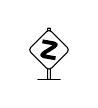
\begin{tikzpicture}[baseline=(x.base)]
		\draw[rounded corners=.01em] (-.05em,-1.07em)rectangle(.05em,.78em);
		\draw[fill=white,rounded corners=1.3] (0,.75em)--(.75em,0)--(0,-.75em)--(-.75em,0)--cycle;
		\draw[line width=0.2mm, line cap=round](-.4em,-1.07em)--(.4em,-1.07em);
		\node(x) at (0,0em) {};
		% Thank you https://tex.stackexchange.com/a/262510
		\draw[
			line cap=but,
			line join=round,
			x=.5em,
			line width=0.5mm,
			y=1*(height("Z")-\pgflinewidth)*(1-sin(10)),
			rotate=-10,
			rounded corners=1.5pt,
		](-0.57, 0.57) -- (0.57, 0.57) -- (-0.57, -0.57) -- (0.57, -0.57);
	\end{tikzpicture}%
}
%%%%%%%%%%%%%%%%%%%%%%%%%%%%%%%%%%%%%%%%%%%% /DANGERS

%%%%%%%%%%%%%%%%%%%%%%%%%%%%%%%%%%%%%%%%%%%% MARGINS
\usepackage{marginnote}
% Thank you https://tex.stackexchange.com/a/472882
% Makes marginnotes always appear on the left, apparently
%
\makeatletter
\long\def\@mn@@@marginnote[#1]#2[#3]{%
	\begingroup
		\ifmmode\mn@strut\let\@tempa\mn@vadjust\else
			\if@inlabel\leavevmode\fi
			\ifhmode\mn@strut\let\@tempa\mn@vadjust\else\let\@tempa\mn@vlap\fi
		\fi
		\@tempa{%
			\vbox to\z@{%
				\vss
				\@mn@margintest
				\if@reversemargin\if@tempswa
						\@tempswafalse
					\else
						\@tempswatrue
				\fi\fi

					\llap{%
						\vbox to\z@{\kern\marginnotevadjust\kern #3
							\vbox to\z@{%
								\hsize\marginparwidth
								\linewidth\hsize
								\kern-\parskip
								%\mn@parboxrestore
								\marginfont\raggedleftmarginnote\strut\hspace{\z@}%
								\ignorespaces#1\endgraf
								\vss
							}%
							\vss
						}%
						\if@mn@verbose
							\PackageInfo{marginnote}{xpos seems to be \@mn@currxpos}%
						\fi
						\begingroup
							\ifx\@mn@currxpos\relax\else\ifx\@mn@currpos\@empty\else
									\kern\@mn@currxpos
							\fi\fi
							\ifx\@mn@currpage\relax
								\let\@mn@currpage\@ne
							\fi
							\if@twoside\ifodd\@mn@currpage\relax
									\kern-\oddsidemargin
								\else
									\kern-\evensidemargin
								\fi
							\else
								\kern-\oddsidemargin
							\fi
							\kern-1in
						\endgroup
						\kern\marginparsep
					}%
			}%
		}%
	\endgroup
}
\makeatother
%
% Mostly for todonotes
\renewcommand{\marginpar}{\marginnote}
%%%%%%%%%%%%%%%%%%%%%%%%%%%%%%%%%%%%%%%%%%%% /MARGINS

%%%%%%%%%%%%%%%%%%%%%%%%%%%%%%%%%%%%%%%%%%%% LISTS
% Putting these into an environment decreases clicking
\newlist{listalph}{enumerate}{1}
\setlist[listalph,1]{label=(\alph*)}
\newlist{listroman}{enumerate}{1}
\setlist[listroman,1]{label=(\roman*)}
%%%%%%%%%%%%%%%%%%%%%%%%%%%%%%%%%%%%%%%%%%%% /LISTS

%%%%%%%%%%%%%%%%%%%%%%%%%%%%%%%%%%%%%%%%%%%% LISTINGS
\usepackage{courier}
\usepackage{listings}
\lstset{basicstyle=\ttfamily,breaklines=true}
%%%%%%%%%%%%%%%%%%%%%%%%%%%%%%%%%%%%%%%%%%%% /LISTINGS

%%%%%%%%%%%%%%%%%%%%%%%%%%%%%%%%%%%%%%%%%%%% THM BOXES
% See http://texdoc.net/texmf-dist/doc/latex/thmtools/thmtools.pdf
\renewcommand{\qedsymbol}{$\blacksquare$}
\usepackage{thmtools,thm-restate}

\usepackage[framemethod=TikZ]{mdframed}
% Fixing mdframed skip below
% See https://tex.stackexchange.com/a/292090/143086
\usepackage[framemethod=TikZ]{mdframed}
\usepackage{xpatch}
\makeatletter
\xpatchcmd{\endmdframed}
	{\aftergroup\endmdf@trivlist\color@endgroup}
	{\endmdf@trivlist\color@endgroup\@doendpe}
	{}{}
\makeatother

\iftoggle{nirfancy}
{
	\definecolor{nirlightblue}{HTML}{f7f7ff}
	\definecolor{nirdarkblue}{HTML}{1d1dbf}
	\declaretheoremstyle[
		mdframed={
			backgroundcolor=nirlightblue,
			linecolor=nirdarkblue,
			rightline=false,
			topline=false,
			bottomline=false,
			linewidth=2pt,
			innertopmargin=5pt,
			innerbottommargin=8pt,
			innerleftmargin=8pt,
			leftmargin=-2pt,
			skipbelow=2pt,
			nobreak
		},
		headfont=\normalfont\bfseries\color{nirdarkblue}
	]{nirbluebox}
}
{
	\declaretheoremstyle[bodyfont=\itshape]{nirbluebox}
}
% I want to label things by chapter, but not all things I write have chapter
\ifx\thechapter\undefined
	\declaretheorem[style=nirbluebox,name=Theorem,within=subsection]{thm}
\else
	\declaretheorem[style=nirbluebox,name=Theorem,within=chapter]{thm}
\fi
\declaretheorem[style=nirbluebox,name=Theorem,numbered=no]{thm*}
\declaretheorem[style=nirbluebox,name=Theorem,sibling=thm]{theorem}
\declaretheorem[style=nirbluebox,name=Theorem,numbered=no]{theorem*}
\declaretheorem[style=nirbluebox,name=Proposition,sibling=thm]{prop}
\declaretheorem[style=nirbluebox,name=Proposition,numbered=no]{prop*}
\declaretheorem[style=nirbluebox,name=Proposition,sibling=thm]{proposition}
\declaretheorem[style=nirbluebox,name=Proposition,numbered=no]{proposition*}
\declaretheorem[style=nirbluebox,name=Problem,numberwithin=section]{prob}
\declaretheorem[style=nirbluebox,name=Lemma,sibling=thm]{lem}
\declaretheorem[style=nirbluebox,name=Lemma,numbered=no]{lem*}
\declaretheorem[style=nirbluebox,name=Lemma,sibling=thm]{lemma}
\declaretheorem[style=nirbluebox,name=Lemma,numbered=no]{lemma*}
\declaretheorem[style=nirbluebox,name=Corollary,sibling=thm]{cor}
\declaretheorem[style=nirbluebox,name=Corollary,numbered=no]{cor*}
\declaretheorem[style=nirbluebox,name=Corollary,sibling=thm]{corollary}
\declaretheorem[style=nirbluebox,name=Corollary,numbered=no]{corollary*}

\iftoggle{nirfancy}
{
	\definecolor{nirlightred}{RGB}{250, 220, 220}
	\definecolor{nirdarkred}{HTML}{f40000}
	\declaretheoremstyle[
		mdframed={
			backgroundcolor=nirlightred,
			linecolor=nirdarkred,
			rightline=false,
			topline=false,
			bottomline=false,
			linewidth=2pt,
			innertopmargin=5pt,
			innerbottommargin=8pt,
			innerleftmargin=8pt,
			leftmargin=-2pt,
			skipbelow=2pt,
			nobreak
		},
		headfont=\normalfont\bfseries\color{nirdarkred}
	]{nirredbox}
}
{
	\declaretheoremstyle[bodyfont=\itshape]{nirredbox}
}
\declaretheorem[style=nirredbox,name=Conjecture,sibling=thm]{conj}
\declaretheorem[style=nirredbox,name=Conjecture,numbered=no]{conj*}
\declaretheorem[style=nirredbox,name=Question,sibling=thm]{ques}
\declaretheorem[style=nirredbox,name=Question,numbered=no]{ques*}
\declaretheorem[style=nirredbox,name=Convention,sibling=thm]{conv}
\declaretheorem[style=nirredbox,name=Convention,numbered=no]{conv*}
\declaretheorem[style=nirredbox,name=Convention,sibling=thm]{convention}
\declaretheorem[style=nirredbox,name=Convention,numbered=no]{convention*}

\makeatletter
\declaretheorem[
	style=nirredbox,
	name=Idea,
	sibling=thm,
	% without phantom{}, the first item in a list gets misformatted \todo{implement https://tex.stackexchange.com/questions/630889/marginnote-eats-first-item-in-thmtools-mdframed?noredirect=1#comment1600939_630889}
	postheadhook={\phantom{}\marginnote{\nirideasymbol}[-3pt]%
	\ifthmt@thisistheone% restatable makes alignment weird
		\hspace{-2.2pt}%
	\else%
		{}%
	\fi}
]{idea}
\declaretheorem[
	style=nirredbox,
	name=Warning,
	sibling=thm,
	% without phantom{}, the first item in a list gets misformatted
	postheadhook={\phantom{}\marginnote{\nirwarnsymbol}[-3pt]%
	\ifthmt@thisistheone% restatable makes alignment weird
		\hspace{-2.2pt}%
	\fi}
]{warn}
\makeatother

\iftoggle{nirfancy}
{
	\definecolor{nirdarkgreen}{HTML}{20660a}
	\definecolor{nirlightgreen}{HTML}{ebffeb}
	\declaretheoremstyle[
		mdframed={
			backgroundcolor=nirlightgreen,
			linecolor=nirdarkgreen,
			rightline=false,
			topline=false,
			bottomline=false,
			linewidth=2pt,
			innertopmargin=5pt,
			innerbottommargin=8pt,
			innerleftmargin=8pt,
			leftmargin=-2pt,
			skipbelow=2pt,
			nobreak
		},
		headfont=\normalfont\bfseries\color{nirdarkgreen}
	]{nirgreenbox}
}
{
	\declaretheoremstyle[bodyfont=\itshape]{nirgreenbox}
}
\declaretheorem[style=nirgreenbox,name=Axiom,sibling=thm]{ax}
\declaretheorem[style=nirgreenbox,name=Axiom,numbered=no]{ax*}
\declaretheorem[style=nirgreenbox,name=Axiom,sibling=thm]{axiom}
\declaretheorem[style=nirgreenbox,name=Axiom,numbered=no]{axiom*}
\declaretheorem[style=nirgreenbox,name=Inventory,sibling=thm]{inv}
\declaretheorem[style=nirgreenbox,name=Inventory,numbered=no]{inv*}
\declaretheorem[style=nirgreenbox,name=Inventory,sibling=thm]{inventory}
\declaretheorem[style=nirgreenbox,name=Inventory,numbered=no]{inventory*}
\declaretheorem[style=nirgreenbox,name=Notation,sibling=thm]{notation}
\declaretheorem[style=nirgreenbox,name=Notation,numbered=no]{notation*}
\declaretheorem[style=nirgreenbox,name=Definition,sibling=thm]{defihelper}
\declaretheorem[style=nirgreenbox,name=Definition,numbered=no]{defihelper*}

\iftoggle{nirfancy}
{
	\definecolor{nirdarkcyan}{HTML}{25805e}
	\definecolor{nirlightcyan}{HTML}{edfffb}
	\declaretheoremstyle[
		mdframed={
			backgroundcolor=nirlightcyan,
			linecolor=nirdarkcyan,
			rightline=false,
			topline=false,
			bottomline=false,
			linewidth=2pt,
			innertopmargin=5pt,
			innerbottommargin=8pt,
			innerleftmargin=8pt,
			leftmargin=-2pt,
			skipbelow=2pt,
			nobreak
		},
		headfont=\normalfont\bfseries\color{nirdarkcyan}
	]{nircyanbox}
}
{
	\declaretheoremstyle[bodyfont=\itshape]{nircyanbox}
}
\declaretheorem[style=nircyanbox,name=Example,sibling=thm]{ex}
\declaretheorem[style=nircyanbox,name=Example,numbered=no]{ex*}
\declaretheorem[style=nircyanbox,name=Example,sibling=thm]{example}
\declaretheorem[style=nircyanbox,name=Example,numbered=no]{example*}
\declaretheorem[style=nircyanbox,name=Non-Example,sibling=thm]{nex}
\declaretheorem[style=nircyanbox,name=Non-Example,numbered=no]{nex*}
\declaretheorem[style=nircyanbox,name=Non-Definition,sibling=thm]{ndefi}
\declaretheorem[style=nircyanbox,name=Non-Definition,numbered=no]{ndefi*}
\declaretheorem[style=nircyanbox,name=Exercise,sibling=thm]{exercise}
\declaretheorem[style=nircyanbox,name=Exercise,numbered=no]{exercise*}
\declaretheorem[style=nircyanbox,name=Exercise,sibling=thm]{exe}
\declaretheorem[style=nircyanbox,name=Exercise,numbered=no]{exe*}

\iftoggle{nirfancy}
{
	\definecolor{nirlightbrown}{RGB}{252,240,235}
	\definecolor{nirdarkbrown}{HTML}{7a5342}
	\declaretheoremstyle[
		mdframed={
			backgroundcolor=nirlightbrown,
			linecolor=nirdarkbrown,
			rightline=false,
			topline=false,
			bottomline=false,
			linewidth=2pt,
			innertopmargin=5pt,
			innerbottommargin=8pt,
			innerleftmargin=8pt,
			leftmargin=-2pt,
			skipbelow=2pt,
			nobreak
		},
		headfont=\normalfont\bfseries\color{nirdarkbrown}
	]{nirbrownbox}
}
{
	\declaretheoremstyle[bodyfont=\itshape]{nirbrownbox}
}
\declaretheorem[style=nirbrownbox,name=Remark,sibling=thm]{remark}
\declaretheorem[style=nirbrownbox,name=Remark,numbered=no]{remark*}
\declaretheorem[style=nirbrownbox,name=Quote,sibling=thm]{quot}
\declaretheorem[style=nirbrownbox,name=Quote,numbered=no]{quot*}
%%%%%%%%%%%%%%%%%%%%%%%%%%%%%%%%%%%%%%%%%%%% /THM BOXES

%%%%%%%%%%%%%%%%%%%%%%%%%%%%%%%%%%%%%%%%%%%% INDEX BOXES
% smuggle the note from the header formatting
\makeatletter
\def\thmt@setheadstyle#1{%
	\thmt@style@headstyle{%
		\def\NAME{\the\thm@headfont ##1}%
		\def\NUMBER{\bgroup\@upn{##2}\egroup}%
		\def\NOTE{\if=##3=\else\bgroup\thmt@space\the\thm@notefont(##3)\egroup\fi}%
		% my precious!
		\def\NIRNOTE{\if=##3=\else##3\fi}%
	}%
	\def\thmt@tmp{#1}%
	\@onelevel@sanitize\thmt@tmp
	%\tracingall
	\ifcsname thmt@headstyle@\thmt@tmp\endcsname
		\thmt@style@headstyle\@xa{%
			\the\thmt@style@headstyle
			\csname thmt@headstyle@#1\endcsname
		}%
	\else
		\thmt@style@headstyle\@xa{%
			\the\thmt@style@headstyle
			#1%
		}%
	\fi
	%\showthe\thmt@style@headstyle
}
% disable indexing in restatable, as with labels
\renewenvironment{thmt@restatable}[3][]{%
	\thmt@toks{}% will hold body
%
	\stepcounter{thmt@dummyctr}% used for data storage label.
%
	\long\def\thmrst@store##1{%
		\@xa\gdef\csname #3\endcsname{%
			\@ifstar{%
				\thmt@thisistheonefalse\csname thmt@stored@#3\endcsname
			}{%
				\thmt@thisistheonetrue\csname thmt@stored@#3\endcsname
			}%
		}%
		\@xa\long\@xa\gdef\csname thmt@stored@#3\@xa\endcsname\@xa{%
			\begingroup
			\ifthmt@thisistheone
				% these are the valid numbers, store them for the other
				% occasions.
				\thmt@rst@storecounters{#3}%
			\else
				% this one should use other numbers...
				% first, fake the theorem number.
				\@xa\protected@edef\csname the#2\endcsname{%
					\thmt@trivialref{thmt@@#3}{??}}%
				% if the number wasn't there, have a "re-run to get labels right"
				% warning.
				\ifcsname r@thmt@@#3\endcsname\else
					\G@refundefinedtrue
				\fi
				% prevent stepcountering the theorem number,
				% but still, have some number for hyperref, just in case.
				\@xa\let\csname c@#2\endcsname=\c@thmt@dummyctr
				\@xa\let\csname theH#2\endcsname=\theHthmt@dummyctr
				% disable labeling.
				\let\label=\thmt@gobble@label
				% disable indexing!
				\let\index=\@gobble
				\let\ltx@label=\@gobble% amsmath needs this
				% We shall need to restore the counters at the end
				% of the environment, so we get
				% (4.2) [(3.1 from restate)] (4.3)
				\def\thmt@restorecounters{}%
				\@for\thmt@ctr:=\thmt@innercounters\do{%
					\protected@edef\thmt@restorecounters{%
						\thmt@restorecounters
						\protect\setcounter{\thmt@ctr}{\arabic{\thmt@ctr}}%
					}%
				}%
				% pull the new semi-static definition of \theequation et al.
				% from the aux file.
				\thmt@trivialref{thmt@@#3@data}{}%
			\fi
			% call the proper begin-env code, possibly with optional argument      
			% (omit if stored via key-val)
			\ifthmt@restatethis
				\thmt@restatethisfalse
			\else
				\csname #2\@xa\endcsname\ifx\@nx#1\@nx\else[{#1}]\fi
			\fi
			\ifthmt@thisistheone
				% store a label so we can pick up the number later.
				\label{thmt@@#3}%
			\fi
			% this will be the collected body.
			##1%
			\csname end#2\endcsname
			% if we faked the counter values, restore originals now.
			\ifthmt@thisistheone\else\thmt@restorecounters\fi
			\endgroup
		}% thmt@stored@#3
		% in either case, now call the just-created macro,
		\csname #3\@xa\endcsname\ifthmt@thisistheone\else*\fi
		% and artificially close the current environment.
		\@xa\end\@xa{\@currenvir}
	}% thm@rst@store
	\thmt@collect@body\thmrst@store
}{%
	%% now empty, just used as a marker.
}
\makeatother
\iftoggle{nirfancy}
{
	\declaretheoremstyle[
		mdframed={
			backgroundcolor=nirlightgreen,
			linecolor=nirdarkgreen,
			rightline=false,
			topline=false,
			bottomline=false,
			linewidth=2pt,
			innertopmargin=5pt,
			innerbottommargin=8pt,
			innerleftmargin=8pt,
			leftmargin=-2pt,
			skipbelow=2pt,
			nobreak
		},
		headfont=\normalfont\bfseries\color{nirdarkgreen},
		headformat={\NAME\ \NUMBER\NOTE{\nirindex{\NIRNOTE}}}
	]{nirgreenboxindexed}
}
{
	\declaretheoremstyle[bodyfont=\itshape]{nirgreenboxindexed}
}
\declaretheorem[style=nirgreenboxindexed,name=Definition,sibling=thm]{defi}
\declaretheorem[style=nirgreenboxindexed,name=Definition,numbered=no]{defi*}
\declaretheorem[style=nirgreenboxindexed,name=Definition,sibling=thm]{definition}
\declaretheorem[style=nirgreenboxindexed,name=Definition,numbered=no]{definition*}
%%%%%%%%%%%%%%%%%%%%%%%%%%%%%%%%%%%%%%%%%%%% /INDEX BOXES
% Bibliography
\usepackage[backend=biber,
    style=alphabetic,
    sorting=ynt
]{biblatex}
\addbibresource{bib.bib}

\title{Intertwining Operators for Siegel Parabolics over Finite Fields} 
\author{Nir Elber and Hahn Lheem}
% \date{Summer 2023}
\date{\today}

\begin{document}

\begin{abstract}
    We consider degenerate principal series representations $\Ind_P^G\chi$ over finite fields, where $G$ is a classical group of even rank, and $P$ is the Siegel parabolic subgroup. For example, we show that this representation is multiplicity-free and irreducible for most characters $\chi$. We then discuss a particular intertwining operator $I$ on $\Ind_P^G\chi$ and its related combinatorics. Firstly, this operator $I$ produces families of diagonalizable antitriangular matrices with well-behaved eigenvalues. Secondly, applying $I$ to a special vector in $\Ind_P^G\chi$ leads us to various matrix Gauss sums, whose evaluations imply an explicit equidistribution result of the trace and determinant of symmetric and alternating invertible matrices.
\end{abstract}

\maketitle

% joint equidistribution of trace and inverse trace
% open double coset?

\tableofcontents

\section{Introduction}
Let $q$ be a prime-power not divisible by $2$ or $3$, and let $2n$ be a positive even integer. For the purposes of the introduction, we work with the group $G\coloneqq\op{SL}_{2n}(\FF_q)$, and we let $P\subseteq G$ denote the subgroup of matrices of the form $\begin{bsmallmatrix}
    A & B \\ & D
\end{bsmallmatrix}$ where $A,B,D\in\FF_q^{n\times n}$. This paper is interested in the degenerate principal series representations $\Ind_P^G\chi$, where $\chi\colon P\to\CC^\times$ is some character, and the combinatorics attached to these representations. We take a moment to remark that these representations play a prominent role in the doubling method of Piatetski-Shapiro and Rallis \cite{ps-r-doubling}; we refer to \Cref{rem:double} at the end of the introduction for some more discussion of this once we have set up the relevant objects.

For example, we are able to show that the representation $\Ind_P^G\chi$ tends to be irreducible.
\begin{theorem}
    The representation $\Ind_P^G\chi$ is multiplicity-free. Furthermore, the number of irreducible components equals
    \[\begin{cases}
        1 & \text{if }\chi^2\ne1, \\
        2 & \text{if }\chi^2=1\text{ but }\chi\ne1, \\
        n+1 & \text{if }\chi=1.
    \end{cases}\]
\end{theorem}
The result follows by combining \Cref{prop:ind-irred,prop:ind-mult-free}. In short, we use Gelfand pairs to show that the representation is multiplicity-free, and we use Mackey theory to compute the number of irreducible components.

The combinatorics attached to this representation comes from defining a special intertwining operator $I\colon\Ind_P^G\chi\to\Ind_P^G\chi'$ by
\[If(g)\coloneqq\sum_{B\in\FF_q^{n\times n}}f\left(\begin{bmatrix}
    & 1_n \\ -1_n
\end{bmatrix}\begin{bmatrix}
    1_n & B \\ & 1_n
\end{bmatrix}g\right),\]
where $\chi'\colon P\to\CC^\times$ is some other explicitly defined character. In general, one has that $I\circ I$ is an operator on $\Ind_P^G\chi$; when $\chi^2=1$, it turns out that $\chi'=\chi$ so that $I$ is an operator on $\Ind_P^G\chi$.

As such, we see that there are two cases of interest for our operator $I$. On one hand, in the exceptional cases where $\chi^2=1$, we can ask how $I$ acts on the irreducible components of $\Ind_P^G\chi$. For simplicity, we will consider $\chi=1$ for the time being. By choosing a basis of $\Ind_P^G1$, we show the following in \Cref{prop:trivial-matrix-coeffs} and \Cref{thm:eigens-gl}.
\begin{theorem} \label{thm:sln-eigens}
    One can give $\Ind_P^G1$ an ordered basis so that the operator $I$ on $\Ind_P^G1$ has matrix given by
    \[\left[(-1)^{i+j-n}q^{n^2-i^2+\binom{i+j-n}2}\frac{(q;q)_i^2}{(q;q)_{n-j}^2(q;q)_{i+j-n}}\right]_{i+j\ge n},\]
    where $(a;q)_n\coloneqq\prod_{i=0}^{n-1}\left(1-aq^i\right)$ is the $q$-Pochhammer symbol; here, $i,j\in\{0,\ldots,n\}$ are indices, and $i+j\ge n$ indicates that the matrix has $0$s when $i+j< n$. This matrix is diagonalizable and has eigenvalues given by
    \[\left\{(-1)^{n-i}q^{\binom n2+\binom{i+1}2}:0\le i\le n\right\}.\]
\end{theorem}
% \begin{example}
%     For $n=4$, this matrix is
%     \[\begin{bmatrix}  &   &   &   & q^{16}\\  &   &   & q^{15}  & \frac{ ( q - 1 ) }{1} q^{15}\\  &   & q^{12}  & \frac{ ( q^{2} - 1 ) ^{2} }{ ( q - 1 ) } q^{12}  & \frac{ ( q - 1 ) ( q^{2} - 1 ) }{1} q^{13}\\  & q^{7}  & \frac{ ( q^{3} - 1 ) ^{2} }{ ( q - 1 ) } q^{7}  & \frac{ ( q^{2} - 1 ) ( q^{3} - 1 ) ^{2} }{ ( q - 1 ) } q^{8}  & \frac{ ( q - 1 ) ( q^{2} - 1 ) ( q^{3} - 1 ) }{1} q^{10}\\1 & \frac{ ( q^{4} - 1 ) ^{2} }{ ( q - 1 ) }  & \frac{ ( q^{3} - 1 ) ^{2} ( q^{4} - 1 ) ^{2} }{ ( q - 1 ) ( q^{2} - 1 ) } q^{1}  & \frac{ ( q^{2} - 1 ) ( q^{3} - 1 ) ( q^{4} - 1 ) ^{2} }{ ( q - 1 ) } q^{3}  & \frac{ ( q - 1 ) ( q^{2} - 1 ) ( q^{3} - 1 ) ( q^{4} - 1 ) }{1} q^{6}\\\end{bmatrix},\]
%     and the eigenvalues are $\left\{q^{16},-q^{12},q^9,-q^7,q^6\right\}$.
% \end{example}
\begin{remark}
    Considerations with other classical groups $G$ produces other families of diagonalizable antitriangular matrices.
\end{remark}
What is remarkable is that we have produced a family of diagonalizable ``antitriangular'' matrices. We are not aware of any general method to handle such diagonalization problems, and it does not appear clear a priori that the eigenvalues listed above should be so well-behaved. Diagonalizing certain antitriangular (satisfying a ``global antidiagonal property'') matrices have combinatorial applications in \cite{britnell-antitriangular}, and some aspects of our methods can be considered $q$-analogues of their arguments, but the analogy is weak. Notably, the family of matrices considered in \Cref{thm:sln-eigens} does not satisfy the global antidiagonal property.

On the other hand, we may still be interested in the generic case $\chi^2\ne1$. In this case, $\op{Ind}^G_P\chi$ is irreducible, so $I\circ I$ is a scalar. As such, one may simply pick up any nonzero vector in $\op{Ind}^G_P\chi$ and apply $I\circ I$ to it in order to compute this scalar. Executing this strategy leads us to consider the matrix Gauss sums of \cite{kim-gauss-sum}; the following result is \Cref{prop:i-on-psi-eigen}.
\begin{theorem}
    Fix a nontrivial character $\psi\colon\FF_q\to\CC^\times$. For each character $\chi\colon P\to\CC^\times$, we define a vector $f_\chi\in\Ind_P^G\chi$ as supported on matrices of the form $p\begin{bsmallmatrix}
        & -1_n \\ 1_n
    \end{bsmallmatrix}\begin{bsmallmatrix}
        1_n & B \\ & 1_n
    \end{bsmallmatrix}$ for $p\in P$ with value
    \[f_\chi\left(p\begin{bmatrix}
        & -1_n \\ 1_n
    \end{bmatrix}\begin{bmatrix}
        1_n & B \\ & 1_n
    \end{bmatrix}\right)\coloneqq\chi(p)\psi(\tr B).\]
    Then
    \[If_\chi=\Bigg(\sum_{B\in\GL_n(\FF_q)}\chi(\det B)\psi(\tr B)\Bigg)f_{\chi'}.\]
\end{theorem}
\begin{remark}
    In fact, even when $I$ fails to be a scalar, we will be able to show that the eigenvalue given by the Gauss sum equals the smallest eigenvalue of $I$, and it seems to be the case that this eigenvalue has the largest eigenspace in $\Ind_P^G\chi$. This is discussed further in \Cref{rem:generic-eigenvalue}. It would be interesting to explicitly compute (or at least compare) the dimensions of all the eigenspaces of $\op{Ind}_P^G\chi$, but this seems out of reach at the moment.
\end{remark}

Thus, we are motivated to evaluate these Gauss sums. In the case of $G=\SL_{2n}(\FF_q)$, the corresponding Gauss sums given as above have been evaluated in \cite{kim-gauss-sum}. However, considerations of other groups $G$ lead to different sums. For example, $G=\Sp_{2n}(\FF_q)$ leads to a sum over invertible symmetric matrices considered in \cite{saito-sym-gauss-sum}, and $G=\O_{4n}(\FF_q)$ leads to a sum over invertible alternating matrices (which appears to be new).

We provide evaluations for all of these matrix Gauss sums. Our methods are based on an explicit row-reduction analogous to the Bruhat decomposition methods of \cite{kim-gauss-sum}, but the explicit nature of our exposition allows our proofs to be rather uniform over all the various sums. For example, even though the sum over invertible symmetric matrices has already been considered in \cite{saito-sym-gauss-sum}, our method seems to be easier to visualize.

Evaluating these Gauss sums also has a combinatorial application: we are able to provide an explicit formula for the number of invertible symmetric, alternating, or general matrices with given trace and determinant. For general invertible matrices, this application is essentially implicit in \cite[Theorem~6.2]{kim-gauss-sum}, so we only state results for symmetric and alternating matrices, which appear to be new. The following results follow from \Cref{cor:count-sym,cor:count-alt}, and they provide an explicit equidistribution result for the trace and determinant.
\begin{theorem}
    Fix $d\in\FF_q^\times$ and $t\in\FF_q$. For odd integers $2m+1$, the number $N(d,t)$ of symmetric $A\in\GL_{2m+1}(\FF_q)$ with $(\det A,\tr A)=(d,t)$ is bounded by
    \[\left|N(d,t)-\frac N{q(q-1)}\right|\le q^{m(m+1)}(q-1)^{m+1},\]
    where $N$ is the total number of invertible symmetric $(2m+1)\times(2m+1)$ matrices.
\end{theorem}
\begin{remark}
    There is analogous, albeit slightly more complicated, result for even integers $2m$.
\end{remark}
\begin{theorem}
    Fix a square $d\in\FF_q^{\times2}$ and $t\in\FF_q$. For even integers $2m$, the number $N(d,t)$ of alternating $A\in\GL_{2m}(\FF_q)$ with $(\det A,\tr A)=(d,t)$ is bounded by
    \[\left|N(d,t)-\frac N{q(q-1)/2}\right|\le q^{m(m-1)}(q-1)^m,\]
    where $N$ is the total number of invertible alternating $2m\times2m$ matrices.
\end{theorem}
\begin{remark} \label{rem:double}
    The aforementioned matrix Gauss sums also appear in finite-field analogues of the doubling method. In short, the doubling method is a way to define gamma factors of representations of groups $G$, and the main idea is to embed the group $G$ (such as $\GL_n(\FF_q)$) into a group $H$ of the same type but twice the size (such as $\GL_{2n}(\FF_q)$). Then for any irreducible representation $\pi$ of $G$ and ``generic'' character $\chi$ of $G$, one can try to prove a multiplicity one theorem
    \[\dim\op{Hom}_{G\times G}\left(\op{Ind}_P^H\chi\otimes\pi\otimes\pi^\lor,\CC\right)=1,\]
    where $P\subseteq H$ is a Siegel parabolic. This allows one to define a zeta function $Z(f,v,w)$ for $\pi$. The intertwining operator $I$ above enters the picture by providing a functional equation for $Z$, and this functional equation defines a gamma factor $\Gamma(\pi,\omega)$.
    
    However, to normalize this gamma factor, one needs to normalize the intertwining operator, which is tantamount to rescaling it so that $I\circ I$ has an eigenspace with eigenvalue of magnitude $1$. Thus, we are once again motivated to understand the eigenvalues of $I$, and we note that matrix Gauss sums in particular provide a clean way to normalize $I$ when $\chi$ is generic; see for example \cite[Section~3.6]{chang-doubling}.
    We refer to \cite{chang-doubling} for more details.
\end{remark}

\subsection{Layout}
We quickly explain the outline of the paper. In \Cref{sec:rep-theory}, we examine the representation theory of $\Ind_P^G\chi$ and explain where the combinatorial applications arise. In \Cref{sec:qcombo}, we provide the diagonalization of our intertwining operator. Lastly, in \Cref{sec:gsum}, we evaluate our matrix Gauss sums and provide the combinatorial applications.

\subsection{Acknowledgements}
This research was conducted during the University of Michigan REU during the summer of 2023; it was funded by the NSF RTG Number Theory and Representation Theory grant. The authors are particularly indebted to his advisors Elad Zelingher and Jialiang Zou for endlessly helpful advice and guidance in many aspects of this paper, from suggestions on the Hecke algebra to a plethora of helpful references. This project could not exist without them. The authors are also grateful to Ofir Gorodetsky for aide in proving certain $q$-identities used in the article, most notably by explaining how to use the packages \texttt{qZeil} and \texttt{qMultiSum}. As such, the authors are also grateful to the Research Institute for Symbolic Computation for access to those two packages.

The first author would also like to thank various friends in the undergraduate mathematics department at the University of California at Berkeley, in particular Jad Damaj, Sophie McCormick, and Zain Shields for diverting conversations regarding diagonalizing antitriangular matrices. Lastly, the first author is most thankful to Hui Sun for consistent companionship.

% !TEX root = ../intertwining.tex

\section{Group-Theoretic Set-Up} \label{sec:rep-theory}
In this section, we set up the necessary representation theory to proceed with the results in the rest of the paper.

\subsection{Groups and Subgroups}
Let $q$ be an odd prime-power, and let $2n$ be a positive even integer; for convenience, we will take $3\nmid q$, but this is used infrequently. Throughout, $G$ will be one of the groups $\{{\GL}_{2n},{\SL}_{2n},\GO_{2n},\O_{2n},\GSp_{2n},\Sp_{2n}\}$ over the finite field $\FF_q$. To explicate our orthogonal and symplectic groups, we fix
\[\varepsilon\coloneqq\begin{cases}
    +1 & \text{if }G\in\{\GO_{2n},\O_{2n}\}, \\
    -1 & \text{if }G\in\{\GSp_{2n},\Sp_{2n}\},
\end{cases}\qquad\text{and}\qquad J\coloneqq\begin{bmatrix}
    & \varepsilon1_n \\
    1_n
\end{bmatrix}\]
so that $G$ is defined to preserve the quadratic form $J$. In the cases where $G\in\{\GL_{2n},\SL_{2n}\}$, it will be convenient to define $\varepsilon\coloneqq-1$ as well. Here, the blank entries in $J$ indicate zeroes, a convention that will stay in place for the rest of the article. Throughout, when there are multiple groups $G$ involved, we will use a superscript $(\cdot)^G$ to distinguish between multiple elements; for example, $\varepsilon^{\GL_{2n}}=-1$.

Note that $G$ has split maximal torus $T$ given by the diagonal matrices. Anyway, the benefit $2n$ being even is that we may use the Siegel parabolic subgroup
\[P\coloneqq\left\{\begin{bmatrix}
    A & B \\
      & D
\end{bmatrix}\in G\right\},\]
where $A,B,C,D$ are implicitly in $\FF_q^{n\times n}$, a convention that will remain in place for any expression in block matrix form as above. We let $U\subseteq P$ be the unipotent radical of $P$, and we let $M\subseteq P$ be the Levi subgroup so that $P=M\ltimes U$. Explicitly,
\[U=\left\{\begin{bmatrix}
    1_n & B \\
      & 1_n
\end{bmatrix}\in G\right\}\qquad\text{and}\qquad M=\left\{\begin{bmatrix}
    A &   \\
      & D
\end{bmatrix}\in G\right\}.\]
The various cases of $G$ provide more constraints on these subgroups. For example, if $G\in\{\GO_{2n},\O_{2n}\}$, then $B$ above must be alternating; if $G\in\{\GSp_{2n},\Sp_{2n}\}$, then $B$ above must be symmetric. Similarly, if $G=\SL_{2n}$, then $\det D=(\det A)^{-1}$; if $G\in\{\O_{2n},\Sp_{2n}\}$, then $D=A^{-\intercal}$; and if $G\in\{\GO_{2n},\GSp_{2n}\}$, then $D=\lambda A^{-\intercal}$ for some $\lambda\in\FF_q^\times$. A quick computation with the definition of $G$ in the various cases reveals that these are only the constraints.

It will be helpful in the sequel to understand characters of $P$. In all cases, we are able to define a ``Siegel determinant'' $\chi_{\det}\colon P\to\FF_q^\times$ given by
\[\chi_{\det}\left(\begin{bmatrix}
    A & B \\
      & D
\end{bmatrix}\right)\coloneqq(\det D)^{-1}.\]
In the cases $G\in\{\GL_{2n},\GO_{2n},\GSp_{2n}\}$, there is an additional ``multiplier'' $m\colon P\to\FF_q^\times$ given by
\[m\left(\begin{bmatrix}
    A & B \\
      & D
\end{bmatrix}\right)=\det AD\text{ if }G=\GL_{2n},\text{ and }m\left(\begin{bmatrix}
    \lambda A & B \\
      & A^{-\intercal}
\end{bmatrix}\right)\coloneqq\lambda\text{ else}.\]
For the remaining cases of $G$, we will define $m$ to just be the trivial character. Both $\chi_{\det}$ and $m$ are characters by a direct computation. It turns out that these are essentially the only characters.
\begin{lemma} \label{lem:decompose-character}
    Let $\chi\colon P\to\CC$ be a character. Then $\chi=(\alpha\circ m)(\beta\circ\chi_{\det})$ for some characters $\alpha,\beta\colon\FF_q^\times\to\CC$.
\end{lemma}
\begin{proof}
    We will do casework on $G$, but before going any further, we argue (directly) that $\chi$ vanishes on $U$; we will actually show that $U$ is contained in the commutator subgroup $[P,P]$. Well, choose some $B$ such that $u\coloneqq\begin{bsmallmatrix}
        1_n & B \\
        & 1_n
    \end{bsmallmatrix}$ is in $U$. Choosing some $a\in\FF_q^\times$, we note $\begin{bsmallmatrix}
        a1_n \\ & a^{-1}1_n
    \end{bsmallmatrix}\in M$, so we consider the commutator
    \[\begin{bmatrix}
        a1_n \\ & a^{-1}1_n
    \end{bmatrix}\begin{bmatrix}
        1_n & B \\ & 1_n
    \end{bmatrix}\begin{bmatrix}
        a1_n \\ & a^{-1}1_n
    \end{bmatrix}^{-1}\begin{bmatrix}
        1_n & B \\ & 1_n
    \end{bmatrix}^{-1}=\begin{bmatrix}
        1_n & \left(a^2-1\right)B \\ & 1_n
    \end{bmatrix}.\]
    As long as we can choose $a$ such that $a^2-1\in\FF_q^\times$, we can replace $B$ with $\left(a^2-1\right)^{-1}B$ in the above computation to conclude that $u\in[P,P]$. Well, because $3\nmid q$, we may choose $a\coloneqq2$ so that $a^2-1=3$.

    The point of the previous paragraph is that $\chi$ now factors through $P/U=M$, so we may as well consider $\chi$ as a character on $M$. We now proceed with our casework.
    \begin{itemize}
        \item If $G\in\{\GL_{2n},\SL_{2n}\}$, we claim that $\chi$ is also trivial on the subgroup
        \[\left\{\begin{bmatrix}
            A &   \\
              & D
        \end{bmatrix}:\det A=\det D=1\right\}.\]
        Well, fix any such $\begin{bsmallmatrix}
            A \\ & D
        \end{bsmallmatrix}$. Indeed, we are given that $A,D\in\SL_{n}$, so we appeal to the fact that $[\SL_{n},\SL_{n}]=\SL_{n}$ for our $q>3$. Thus, $A$ and $D$ can be expressed as commutators $A=A_1A_2A_1^{-1}A_2^{-1}$ and $D=D_1D_2D_1^{-1}D_2^{-1}$ so that 
        \[\begin{bmatrix}
            A \\ & D
        \end{bmatrix}=\begin{bmatrix}
            A_1 \\ & D_1
        \end{bmatrix}\begin{bmatrix}
            A_2 \\ & D_2
        \end{bmatrix}\begin{bmatrix}
            A_1 \\ & D_1
        \end{bmatrix}^{-1}\begin{bmatrix}
            A_2 \\ & D_2
        \end{bmatrix}^{-1},\]
        so our element is a commutator.
        
        Thus, $\chi$ on $M$ now factors through $M/(\SL_n\times\SL_n)$. If $G=\GL_{2n}$, this quotient is isomorphic to $\FF_q^\times\times\FF_q^\times$ by $\begin{bsmallmatrix}
            A \\ & D
        \end{bsmallmatrix}\mapsto\left(\det AD,\det D^{-1}\right)$, so $\chi$ indeed factors through a product of $m$ and $\chi_{\det}$. On the other hand, if $G=\SL_{2n}$, this quotient is isomorphic to $\FF_q^\times$ just by $\begin{bsmallmatrix}
            A \\ & D
        \end{bsmallmatrix}\mapsto\det D^{-1}$ because we have the condition $\det AD=1$ already, so we again factor through $\chi_{\det}$.

        \item If $G\in\{\GO_{2n},\O_{2n},\GSp_{2n},\Sp_{2n}\}$, we claim that $\chi$ is also trivial on the subgroup
        \[\left\{\begin{bmatrix}
            A \\ & A^{-\intercal}
        \end{bmatrix}:\det A=1\right\}.\]
        Well, fix any such $\begin{bsmallmatrix}
            A \\ & A^{-\intercal}
        \end{bsmallmatrix}$. Again, we are given that $A\in\SL_n$, so we appeal to the fact that $[\SL_{n},\SL_{n}]=\SL_{n}$ for our $q>3$, meaning we may write $A=A_1A_2A_1^{-1}A_2^{-1}$ so that
        \[\begin{bmatrix}
            A \\ & A^{-\intercal}
        \end{bmatrix}=\begin{bmatrix}
            A_1 \\ & A_1^{-\intercal}
        \end{bmatrix}\begin{bmatrix}
            A_2 \\ & A_2^{-\intercal}
        \end{bmatrix}\begin{bmatrix}
            A_1 \\ & A_1^{-\intercal}
        \end{bmatrix}^{-1}\begin{bmatrix}
            A_2 \\ & A_2^{-\intercal}
        \end{bmatrix}^{-1},\]
        so our element is a commutator.

        Thus, $\chi$ now factors through $M/\SL_n$, where $\SL_n$ is embedded into $M$ as the above subgroup. If $G\in\{\O_{2n},\Sp_{2n}\}$, then elements of $M$ look like $\begin{bsmallmatrix}
            A \\ & A^{-\intercal}
        \end{bsmallmatrix}$, so this quotient is isomorphic to $\FF_q^\times$ via $\chi_{\det}$, meaning $\chi$ indeed factors through $\chi_{\det}$. Otherwise, $G\in\{\GO_{2n},\GSp_{2n}\}$, so elements of $M$ look like $\begin{bsmallmatrix}
            \lambda A \\ & A^{-\intercal}
        \end{bsmallmatrix}$, so this quotient is isomorphic to $\FF_q^\times\times\FF_q^\times$ via $(m,\chi_{\det})$, allowing us to conclude again.
        \qedhere
    \end{itemize}
\end{proof}
The lemma now allows us to take any character $\chi\colon P\to\CC^\times$ and define $\alpha_\chi,\beta_\chi\colon\FF_q^\times\to\CC^\times$ such that $\chi=(\alpha_\chi\circ m)(\beta_\chi\circ\chi_{\det})$. When $m$ is trivial, we will take $\alpha_\chi$ to be trivial as well; otherwise, $m$ and $\chi_{\det}$ are surjective, so $\alpha_\chi$ and $\beta_\chi$ are uniquely determined by $\chi$.

\subsection{Some Weyl Group Computations}
An argument similar to \cite[Example~17.88]{milne-alg-group} verifies that the diagonal subgroup $T$ of $G$ is always a maximal torus; namely, one can check that $C_G(T)=T$. Then an argument similar to \cite[Example~17.42]{milne-alg-group} verifies that $N_G(T)$ consists of permutation matrices (up to torus elements); alternatively, one can study the Weyl group of the relevant root system and then convert this back into permutation matrices by hand. In any case, we let $W$ denote the Weyl group of $G$, and we let $W_P$ denote the Weyl group of the Siegel parabolic subgroup $P$.

It will be useful to explicitly compute these Weyl groups explicitly. If $G\in\{\GL_n,\SL_n\}$, then $W$ consists of the permutation matrices up to a sign. For each $w\in W$, we let $\sigma_w\in N_G(T)$ denote the corresponding permutation matrix, and we let $d_w\in T$ be a diagonal matrix with entries in $\pm1$ such that $\det d_w\sigma_w=1$. (The choice of $d_w$ will not matter too much in the sequel.) The point is that $\{d_w\sigma_w\}_{w\in W}$ provides a set of representatives for $W$ in $G$.

We would like a similar description for $G\in\{\GO_{2n},\O_{2n},\GSp_{2n},\Sp_{2n}\}$. The main point of the computation here is to ask which permutation matrices $\sigma$ actually belong to $G$, and then we can again use $d_w$ to correct for the determinant condition.
\begin{lemma} \label{lem:weyl-normal-form}
    Suppose $G\in\{\GO_{2n},\O_{2n},\GSp_{2n},\Sp_{2n}\}$. Let $\Sigma$ be the set of permutations $\sigma\in S_{2n}$ such that $\sigma(i+n)\equiv\sigma(i)+n\pmod{2n}$ for each $i$.
    \begin{enumerate}[label=(\alph*)]
        \item For each $w$ representing a class in $W$, there exists a unique permutation $\sigma\in\Sigma$ such that $w=d\sigma$ for some diagonal matrix $d$.
        \item For each $\sigma\in\Sigma$, there exists some diagonal matrix $d$ with entries in $\{\pm1\}$ such that $d\sigma\in G$. %In fact, $d=\operatorname{diag}(d_1,d_2,\ldots,d_{2n})$ is uniquely determined by the values $\{d_{\sigma(1)},\ldots,d_{\sigma(n)}\}$.
    \end{enumerate}
\end{lemma}
\begin{proof}
    We will show the parts independently.
    \begin{enumerate}[label=(\alph*)]
        \item Recalling that the diagonal matrices of $G$ make up a maximal torus in $B$, we note that diagonal matrices are normalized by the semidirect product of permutation matrices and diagonal matrices (this is even true in $\GL_{2n}$), so we can view elements of $W$ as permutation matrices with elements adjusted by a diagonal element to lie in $G$.
        
        In particular, we may write $w=d\sigma$ for some diagonal matrix $d$, and this $\sigma$ is unique. It remains to show $\sigma\in\Sigma$. Well, the main point is that $d\sigma\in G$ requires
        \[d\sigma J\sigma^\intercal d^\intercal=\lambda J\]
        for some scalar $\lambda$, possibly forced equal to $1$ if $G\in\{\O_{2n},\Sp_{2n}\}$. Setting $d\coloneqq\operatorname{diag}(d_1,\ldots,d_{2n})$, we now pass through a basis vector $e_{\sigma(i)}$ to compute
        \begin{equation}
            \varepsilon^{1_{i>n}}d_{\sigma(i+n)}d_{\sigma(i)}e_{\sigma(i+n)}=\varepsilon^{1_{\sigma(i)>n}}e_{\sigma(i)+n}, \label{eq:test-sigma-in-gsp}
        \end{equation}
        where indices live in $\{1,2,\ldots,2n\}$ but are considered$\pmod{2n}$. Because the diagonal elements of $d$ are nonzero, we must have $\sigma(i+n)\equiv\sigma(i)+n\pmod{2n}$, meaning $\sigma\in\Sigma$.

        \item We need a diagonal matrix $d=\operatorname{diag}(d_1,\ldots,d_{2n})$ such that $d\sigma\in G$, so it is enough for $d\sigma J\sigma^\intercal d^\intercal=J$. Well, it suffices to check this on basis vectors $e_{\sigma(i)}$, for which we see it is enough \eqref{eq:test-sigma-in-gsp}. But because $\sigma\in\Sigma$, it is equivalent to require
        \[\varepsilon^{1_{i>n}}d_{\sigma(i)+n}d_{\sigma(i)}=\varepsilon^{1_{i>n}}d_{\sigma(i+n)}d_{\sigma(i)}=\varepsilon^{1_{\sigma(i)>n}}\]
        for each index $i$. Observe $\varepsilon^{1_{(i+n)>n}}=-\varepsilon^{1_{i>n}}$ and $\varepsilon^{1_{\sigma(i+n)>n}}=-\varepsilon^{1_{\sigma(i)>n}}$ (indices are still taken$\pmod{2n}$), so if the above equation is satisfied at index $i$, then it is satisfied at index $i+n$.
        
        As such, given signs $\{d_{\sigma(1)},\ldots,d_{\sigma(n)}\}$, we must set $d_{\sigma(i)+n}\coloneqq\varepsilon^{1_{\sigma(i)>n}}d_{\sigma(i)}$ for each $i\in\{1,2,\ldots,2\}$ to satisfy the equation at the indices $i\in\{1,2,\ldots,n\}$, and this choice of signs will work.
        \qedhere
    \end{enumerate}
\end{proof}
\begin{remark}
    Let's provide a convenient choice of signs $d_w$ for $w\in W$. If $G\in\{\GO_{2n},\O_{2n}\}$, then $\varepsilon=1$, so we see that $d_w\coloneqq1_{2n}$ will always work. If $G\in\{\GSp_{2n},\Sp_{2n}\}$, then we claim that we can put signs $d_w$ on the top-right quadrant of $\sigma_w$. Explicitly, we take $d_{\sigma(i)}=-1$ if $i\le n$ and $\sigma(i)>n$, and we take $d_{\sigma(i)}=1$ otherwise. The computation of the above lemma shows that this works (note $\varepsilon=-1$).
\end{remark}
Our benefit to having explicit representatives of $W$ is that we get explicit representatives of certain double quotients. For example, $W$ itself provides representatives of $B\backslash G/B$ by the Bruhat decomposition, where $B\subseteq G$ is a Borel subgroup containing $T$. We will be interested in $P\backslash G/P$.
\begin{lemma} \label{lem:compute-pgp}
    For each $r\in\{0,1,\ldots,n\}$, define
    \[\eta_r\coloneqq\begin{bmatrix}
        1_{n-r} \\ &&& \varepsilon1_r \\
        && 1_{n-r} \\
        & 1_r
    \end{bmatrix}.\]
    Then $\{\eta_0,\ldots,\eta_r\}\subseteq G$ provides a set of representatives of the double quotients $P\backslash G/P$.
\end{lemma}
\begin{proof}
    Even though the statement is rather uniform in $G$, the proof will require some moderate casework. Intuitively, what is going on here is that the Weyl group $W_P$ of $P$ consists of permutation matrices in the top-left and bottom-right quadrants, so to compute $P\backslash G/P\cong W_P\backslash W/W_P$, one can correct an arbitrary Weyl element $w\in W$ into the above form by row-reduction into the above form. We will argue slightly more directly.

    Before doing anything serious, we check that $\eta_r\in G$ in all cases. Observe that
    \[\eta_r^\intercal J\eta_r=\begin{bmatrix}
        1_{n-r} \\ &&& 1_r \\
        && 1_{n-r} \\
        & \varepsilon1_r
    \end{bmatrix}\begin{bmatrix}
        && \varepsilon1_{n-r} \\
        &&& \varepsilon1_r \\
        1_{n-r} \\
        & 1_r
    \end{bmatrix}\begin{bmatrix}
        1_{n-r} \\ &&& \varepsilon1_r \\
        && 1_{n-r} \\
        & 1_r
    \end{bmatrix}=J\]
    by a direct computation. So if $\varepsilon=1$, we see $\eta_r\in\O_{2n}$; and if $\varepsilon=-1$, we see $\eta_r\in\Sp_{2n}\subseteq\SL_{2n}$.

    It remains to show that $\{\eta_0,\ldots,\eta_n\}$ provides a set of representatives. We define a function $\rho\colon G\to\{0,\ldots,n\}$ by $\rho\left(\begin{bsmallmatrix}
        A & B \\ C & D
    \end{bsmallmatrix}\right)\coloneqq\op{rank}C$. Note that $\rho$ is surjective because $\rho(\eta_r)=r$ for each $r\in\{0,\ldots,n\}$. We will show that $\rho$ descends to a bijection $P\backslash G/P\to\{0,\ldots,n\}$, from which the result follows because $\rho(\eta_r)=r$.

    To begin, we show that $\rho$ descends to a surjection $P\backslash G/P\to\{0,\ldots,n\}$. Because $\rho$ is already a surjection, we just need to check that $\rho$ is defined up to double cosets. Well, we compute that
    \[\rho\left(\begin{bmatrix}
        A' & B' \\ & D'
    \end{bmatrix}\begin{bmatrix}
        A & B \\ C & D
    \end{bmatrix}\begin{bmatrix}
        A'' & B'' \\ & D''
    \end{bmatrix}\right)=\rho\left(\begin{bmatrix}
        * & * \\
        D'CA'' & *
    \end{bmatrix}\right)=\op{rank}D'CA'',\]
    where $*$ indicates some value we have not bothered to compute. Now, multiplication by an invertible matrix does not adjust rank, so $\op{rank}D'CA''=\op{rank}C=\rho\left(\begin{bsmallmatrix}
        A & B \\ C & D
    \end{bsmallmatrix}\right)$.

    It remains to show that the function $\rho\colon P\backslash G/P\to\{0,
    \ldots,n\}$ is injective. Unwinding definitions, it is enough to show that we must show that $\rho(g)=r$ implies that $g\in P\eta_rP$. Choosing a Borel subgroup $B\subseteq P$ containing $T$, we may use the Bruhat decomposition to see that $B\backslash G/B$ is represented by the Weyl group $W$. Thus, we may assume that $g=w=d_w\sigma_w$ where $d_w\in T$ and $\sigma_w$ is a permutation matrix. Now, to use that $\rho(d_w\sigma_w)=r$, we note that $\sigma_w$ being a permutation matrix means that the rank of the bottom-left quadrant is just
    \[r=\rho(d_w\sigma_w)=\#\{i\le n:\sigma(i)>n\}.\]
    Now, we may choose a permutation $\sigma$ of $\{1,\ldots,n\}$ so that
    \[\{i\in\{1,\ldots,n\}:\sigma_w\sigma(i)>n\}=\{1,\ldots,r\}.\]
    If $G\in\{\GL_{2n},\SL_{2n}\}$, then we extend $\sigma$ to $S_{2n}$ by requiring $\{i>n:\sigma_w\sigma(i)\le n\}=\{n+1,\ldots,n+r\}$. Otherwise, $\sigma$ may be extended to a permutation in $\Sigma$ (from \Cref{lem:weyl-normal-form}), and we can see that $\sigma\in D_{2n}^{\mathrm{sp}}$. Thus, $\sigma$ belongs to some Weyl element in $W\cap P$, so multiplication on the right of $w$ by this Weyl element, we may assume that
    \begin{align*}
        \{i\le n:\sigma_w(i)>n\} &= \{1,\ldots,r\} \\
        \{i>n:\sigma_w(i)>n\} &= \{n+1,\ldots,n+r\}
    \end{align*}
    on the nose. A similar argument by multiplying on the left of $w$ is able to rearrange the actual values of $\sigma_w$ to show that $w$ has the same underlying permutation matrix as $\eta_r$, so $w=\eta_r\in P\eta_rP$ follows.
\end{proof}
\begin{remark}
    A benefit of the above proof with $\rho$ (instead of arguing with $W_P\backslash W/W_P$) is that we see that the double cosets
    \[P\eta_rP=\left\{\begin{bmatrix}
        A & B \\ C & D
    \end{bmatrix}\in G:\op{rank}C=r\right\}\]
    are all (Zariski) locally closed. In fact, $P\eta_0P$ is (Zariski) closed, and $P\eta_rP$ is the only (Zariski) open double coset (defined by $\det C\ne0$).
\end{remark}

% maybe compute P\G/U for the spherical vector, but maybe I'll worry about that later

\subsection{Parabolic Induction}
In the sequel, we will be interested in the representations $\Ind_P^G\chi$ where $\chi\colon P\to\CC^\times$ is a character. We spend this subsection collecting a few facts about these representations. In particular, we will show that these representations are multiplicity-free and irreducible for ``general'' $\chi$.

Let's begin by showing our generic irreducibility.
\begin{proposition} \label{prop:ind-irred}
    Fix a character $\chi\colon P\to\CC^\times$, which we write as $\chi=(\alpha\circ m)(\beta\circ\chi_{\det})$. Then
    \[\dim\End_G\Ind_P^G\chi=\begin{cases}
        n+1 & \text{if }\beta=1, \\
        2 & \text{if }\beta^2=1,\beta\ne1\text{ and }G=\SL_{2n}, \\
        n+1 & \text{if }\beta^2=1,\beta\ne1\text{ and }G\in\{\O_{2n},\Sp_{2n}\}, \\
        \floor{\frac12(n+1)} & \text{if }\beta^2=1,\beta\ne1\text{ and }G\in\{\GO_{2n},\GSp_{2n}\}, \\
        1 & \text{else}.
    \end{cases}\]
    In particular, $\Ind_P^G\chi$ is irreducible provided $\beta^2\ne1$.
\end{proposition}
\begin{proof}
    We use Mackey theory in the form of \cite[Theorem~32.1]{bump-lie-group}. Namely, we are interested in computing the dimension of the space
    \[\mc H\coloneqq\{f\in\op{Mor}(G,\CC):f(p_1gp_2)=\chi(p_1)\chi(p_2)f(g)\text{ for }p_1,p_2\in P,g\in G\}.\]
    Thus, we see that $f\in \mc H$ is uniquely determined by its values on representatives of the double cosets $P\backslash G/P$. As such, we set $f_r\in \mc H$ to be supported on $P\eta_rP$ defined by $f_r(\eta_r)\in\{0,1\}$, where we take $f_r(\eta_r)=1$ provided that this gives a well-defined function in $\mc H$. Then our computation of $P\backslash G/P$ in \Cref{lem:compute-pgp} tells us that $\{f_r:f_r\ne0\}$ is a basis of $\mc H$.

    Thus, we are left computing the number of $r$ such that $f_r\in \mc H$ is well-defined with $f_r(\eta_r)=1$. So fix some $r$, and we check if $f_r\in \mc H$ is well-defined with $f_r(\eta_r)=1$. Namely, if $p_1\eta_rp_2=p_1'\eta_rp_2'$ for $p_1,p_1',p_2,p_2'\in P$, we must check that $\chi(p_1)\chi(p_2)=\chi(p_1')\chi(p_2')$. Rearranging, it is enough to check that $p_1=\eta_rp_2\eta_r^{-1}$ implies that $\chi(p_1)=\chi(p_2)$. In other words, if $p\in P$ has $\eta_rp\eta_r^{-1}\in P$, we need $\chi(p)=\chi\left(\eta_rp\eta_r^{-1}\right)$. Well, we write
    \[p\coloneqq\begin{bmatrix}
        A_1 & A_2 & B_1 & B_2 \\
        A_3 & A_4 & B_3 & B_4 \\
            &     & D_1 & D_2 \\
            &     & D_3 & D_4
    \end{bmatrix}\]
    to have the same dimensions as $\eta_r$, and then we see that
    \begin{align*}
        \eta_rp\eta_r^{-1} &= \begin{bmatrix}
            1_{n-r} \\
            &&& \varepsilon 1_{r} \\
            && 1_{n-r} \\
            & 1_{r}
        \end{bmatrix}\begin{bmatrix}
            A_1 & A_2 & B_1 & B_2 \\
            A_3 & A_4 & B_3 & B_4 \\
                &     & D_1 & D_2 \\
                &     & D_3 & D_4
        \end{bmatrix}\begin{bmatrix}
            1_{n-r} \\
            &&& \varepsilon 1_{r} \\
            && 1_{n-r} \\
            & 1_{r}
        \end{bmatrix}^{-1} \\
        &= \begin{bmatrix}
            A_1 & \varepsilon B_2 &  B_1 & A_2 \\
                &  D_4 & \varepsilon D_3 \\
                & \varepsilon D_2 &  D_1 \\
            A_3 & \varepsilon B_4 &  B_3 & A_4
        \end{bmatrix},
    \end{align*}
    so this is in $P$ if and only if $A_3=B_4=D_2=0$. Thus, $\chi(p)=\chi\left(\eta_rp\eta_r^{-1}\right)$ is equivalent to always having
    \[\chi\left(\begin{bmatrix}
        A_1 & \varepsilon B_2 &  B_1 & A_2 \\
            &  D_4 & \varepsilon D_3 \\
            &      &  D_1 \\
            &      &  B_3 & A_4
    \end{bmatrix}\right)\stackrel?=\chi\left(\begin{bmatrix}
        A_1 & A_2 & B_1 & B_2 \\
            & A_4 & B_3 &     \\
            &     & D_1 &     \\
            &     & D_3 & D_4
    \end{bmatrix}\right).\]
    The multiplier of the left-hand side is $m\left(\eta_rp\eta_r^{-1}\right)=m(p)$, which is also the multiplier of the right-hand side, so we are allowed to ignore $\alpha$ for the rest of the proof. (The point is that $m$ is defined as a character on $G$.) As for $\beta$, we go ahead and compute $\chi_{\det}$ on both sides to see that we must have
    \[\beta(\det D_1\cdot\det A_4)^{-1}\stackrel?=\beta(\det D_1\cdot\det D_4)^{-1},\]
    where we take the convention that the ``empty'' matrix has determinant $1$. Equivalently, we are asking for
    \[\beta(\det A_4)\stackrel?=\beta(\det D_4).\]
    We now work in cases on $G$ and $r$.
    \begin{itemize}
        \item If $r=0$, then $A_4$ and $D_4$ are empty, so the condition holds. Thus, we will take $r>1$ in the rest of our casework.
        \item If $\beta=1$, then the condition holds. Thus, we will take $\beta\ne1$ in the rest of our casework.
        \item Take $G=\GL_{2n}$. Because $r>0$, $\det$ is always surjective, and here there are no conditions on how $\det A_4$ and $\det D_4$ should relate to each other, so the condition never holds.
        \item Take $G=\SL_{2n}$. Because $r>0$, $\det$ will always be surjective. If $r=n$, then the condition $\det p=1$ becomes $\det A_4=\det D_4^{-1}$, so we get a contribution in this case only when $\beta^2=1$. Otherwise, $r\notin\{0,n\}$, so $\det A_4$ and $\det D_4$ can be arbitrary elements of $\FF_q^\times$ (our condition $\det p=1$ only requires $\det A_1D_4D_1A_4=1$), so the condition never holds.
        \item Take $G\in\{\O_{2n},\Sp_{2n}\}$. Then $A_4=D_4^{-\intercal}$, so we are requiring $\beta(\det A_4)^2=1$. Because $\det$ is surjective when $r>0$, nonzero $r$ contribute in this case exactly when $\beta^2=1$.
        \item Take $G\in\{\GO_{2n},\GSp_{2n}\}$. Then $A_4=m(p)D_4^{-\intercal}$, so we are requiring
        \[\beta(\det A_4)^2=\beta(m(p))^r.\]
        With $r>0$, the values $\det A_4$ and $m(p)$ are arbitrary elements of $\FF_q^\times$, so we would like for $\beta(x)^2=\beta(y)^r$ for any $x,y\in\FF_q^\times$. Taking $y=1$ shows that we will only get contributions in this case when $\beta^2=1$, and taking $x=1$ shows that we will only get contributions when $\beta^r=1$ too. However, with $\beta\ne1$, we see that $\beta^r=1$ only happens when $r$ is even.
    \end{itemize}
    Tallying the above cases completes the proof.
\end{proof}
\begin{remark}
    In the sequel, we will make frequent use of the basis of $f_\bullet$s of $\mc H$.
\end{remark}
Even though it is not currently relevant to our discussion, we will want a similar Mackey theory computation in the future, so we will get it out of the way now. We require a definition.
\begin{definition} \label{def:chi-j}
    Note that the element $J$ normalizes $M$: for any $\begin{bsmallmatrix}
		A \\ & D
	\end{bsmallmatrix}\in M$, we see that $J^{-1}\begin{bsmallmatrix}
		A \\ & D
	\end{bsmallmatrix}J=\begin{bsmallmatrix}
		D \\ & A
	\end{bsmallmatrix}\in M$. Thus, for any character $\chi\colon P\to\CC^\times$, we define the character $\chi^J$ as the following composite.
	\[\arraycolsep=1.4pt\begin{array}{cccccccc}
		P &\onto& M &\stackrel J\cong& M &\stackrel\chi\to& \CC^\times \\
		\begin{bsmallmatrix}
			A & B \\ & D
		\end{bsmallmatrix} &\mapsto& \begin{bsmallmatrix}
			A \\ & D
		\end{bsmallmatrix} &\mapsto& \begin{bsmallmatrix}
			D \\ & A 
		\end{bsmallmatrix} &\mapsto& \chi\left(\begin{bsmallmatrix}
			D \\ & A 
		\end{bsmallmatrix}\right)
	\end{array}\]
\end{definition}
\begin{remark}
	The importance of this definition arises in \Cref{lem:parabolic-intertwine}.
\end{remark}
\begin{remark}
	Write $\chi=(\alpha\circ m)(\beta\circ\chi_{\det})$. Then we will evaluate $\chi^J$ on $p\coloneqq\begin{bsmallmatrix}
		A & B \\ & D
	\end{bsmallmatrix}$ as
	\[\chi^J\left(\begin{bmatrix}
		A & B \\ & D
	\end{bmatrix}\right)=\chi\left(\begin{bmatrix}
		D \\ & A
	\end{bmatrix}\right).\]
	If $G\in\{\GL_{2n},\SL_{2n}\}$, then this is $\alpha(\det AD)\beta(\det A)^{-1}=(\alpha/\beta)(\det AD)\beta(\det D)$, so we see that $\chi^J=\left(\alpha\beta^{-1}\circ m\right)\left(\beta^{-1}\circ\chi_{\det}\right)$. Otherwise, if $G\in\{\GO_{2n},\O_{2n},\GSp_{2n},\Sp_{2n}\}$, then we rewrite $p$ as $\begin{bsmallmatrix}
		\lambda A & B \\ & A^{-\intercal}
	\end{bsmallmatrix}$ so that we get $\chi^J(p)=\alpha(\lambda)\beta(\det\lambda A)^{-1}$, so $\chi^J=\left(\alpha\beta^{-n}\circ m\right)\left(\beta^{-1}\circ\chi_{\det}\right)$.
	
	In particular, all cases find that $\left(\chi^J\right)^J=\chi$. Further, if $\beta=1$, then $\chi^J=\chi$; alternatively, if we only have $\beta^2=1$ but $G\in\{\SL_{2n},\O_{2n},\Sp_{2n}\}$ so that $m=1$, then we still have $\chi^J=\chi$.
\end{remark}
\begin{proposition} \label{prop:twisted-ind-basis}
	Fix a character $\chi\colon P\to\CC^\times$, which we write as $\chi=(\alpha\circ m)(\beta\circ\chi_{\det})$. Then we compute a basis for $\left(\Ind_P^G\chi\right)^{\chi^J}$. In particular, we find
	\[\dim\left(\Ind_P^G\chi\right)^{\chi^J}=\dim\left(\Ind_P^G\chi\right)^{\chi}.\]
\end{proposition}
\begin{proof}
	We proceed as in \Cref{prop:ind-irred}. For brevity, set $\mc H_J\coloneqq\left(\Ind_P^G\chi\right)^{\chi^J}$. Again, $f\in\mc H_J$ is uniquely determined by its values on representatives of $P\backslash G/P$, so we set $f_r\in\mc H_J$ to be supported on $P\eta_rP$ defined by $f_r(\eta_r)\in\{0,1\}$ where we take $f_r(\eta_r)=1$ whenever possible; thus, $\{f_r:f_r\ne0\}$ is a basis of $\mc H_J$.

	Continuing, as in \Cref{prop:ind-irred}, we are checking which $f_r\in\mc H_J$ are well-defined with $f_r(\eta_r)=1$. Namely, for $p_1,p_2,p_1',p_2'\in P$, we must have $\chi(p_1)\chi^J(p_2)=f_r(p_1\eta_rp_2)=f_r(p_1'\eta_rp_2')=\chi(p_1')\chi^J(p_2)$. Rearranging, it is enough to check that $p_1=\eta_rp_2\eta_r^{-1}$ implies that $\chi(p_1)=\chi^J(p_2)$. In other words, if $p\in P$ has $\eta_rp\eta_r^{-1}\in P$, we need $\chi(p)=\chi\left(\eta_rp\eta_r^{-1}\right)$. Writing
	\[p\coloneqq\begin{bmatrix}
        A_1 & A_2 & B_1 & B_2 \\
        A_3 & A_4 & B_3 & B_4 \\
            &     & D_1 & D_2 \\
            &     & D_3 & D_4
    \end{bmatrix}\]
    to have the same dimensions as $\eta_r$, and then we see that
    \[\eta_rp\eta_r^{-1} = \begin{bmatrix}
		A_1 & \varepsilon B_2 &  B_1 & A_2 \\
			&  D_4 & \varepsilon D_3 \\
			& \varepsilon D_2 &  D_1 \\
		A_3 & \varepsilon B_4 &  B_3 & A_4
	\end{bmatrix},\]
	so this is in $P$ if and only if $A_3=B_4=D_2=0$. Thus, $\chi(p)=\chi^J\left(\eta_rp\eta_r^{-1}\right)$ is equivalent to always having
	\[\chi\left(\begin{bmatrix}
        A_1 & A_2 & B_1 & B_2 \\
            & A_4 & B_3 &     \\
            &     & D_1 &     \\
            &     & D_3 & D_4
    \end{bmatrix}\right)\stackrel?=\chi^J\left(\begin{bmatrix}
        A_1 & \varepsilon B_2 &  B_1 & A_2 \\
            &  D_4 & \varepsilon D_3 \\
            &      &  D_1 \\
            &      &  B_3 & A_4
    \end{bmatrix}\right).\]
	We now do casework on $G$ and $r$.
	\begin{itemize}
		\item If $G\in\{\O_{2n},\Sp_{2n}\}$, then $\chi^J=\beta^{-1}\circ\chi_{\det}$, so we are asking for
		\[\beta(\det D_1\det D_4)^{-1}\stackrel?=\beta(\det D_1\det A_4).\]
		In this case, $A_4=D_4^{-\intercal}$, so we see that the above is equivalent to $\beta(\det D_1)^2=1$. If $r=n$, then we always get a contribution because $D_1$ is empty; otherwise, $\det$ is surjective, so we get contributions only when $\beta^2=1$.
		\item If $G=\SL_{2n}$, then $\chi^J=\beta^{-1}\circ\chi_{\det}$, so we are still asking for
		\[\beta(\det D_1\det D_4)^{-1}\stackrel?=\beta(\det D_1\det A_4).\]
		This simplifies to
		\[\beta\left(\det A_4\det D_1^2\det D_4\right)=\beta(\det A_1)^{-1}\beta(\det D_1)\stackrel?=1.\]
		Now, if $r=n$, then $A_1$ and $D_1$ is empty, so we are asking for $\beta(\det A_4D_4)=1$, which is true because $\det A_4D_4=1$. If $r=0$, then we must have $\det A_1D_1=1$, so we get a contribution provided $\beta^2=1$. Otherwise, with $r\notin\{0,n\}$, the determinants $\det A_1$ and $\det D_1$ are arbitrary, so we only get a contribution when $\beta=1$.
		\item If $G=\GL_{2n}$, then $\chi^J=\left(\alpha\beta^{-1}\circ m\right)\left(\beta^{-1}\circ\chi_{\det}\right)$, so we are asking for
		\[\alpha\left(\det A_1D_1\det A_4D_4\right)\beta(\det D_1\det D_4)^{-1}=\alpha\beta^{-1}\left(\det A_1D_1\det A_4D_4\right)\beta(\det D_1\det A_4).\]
		Here, we see that $\alpha$ cancels on both sides, so we may ignore it. Rearranging, this is equivalent to
		\[\beta(\det D_1)=\beta\left(\det A_1\right).\]
		If $r=n$, then $D_1$ and $A_4$ are empty, so this condition holds. Otherwise, with $r<n$, these determinants are basically arbitrary, so we only get a contribution when $\beta=1$.
		\item If $G\in\{\GO_{2n},\GSp_{2n}\}$, then $\chi^J=\left(\alpha\beta^{-n}\circ m\right)\left(\beta^{-1}\circ\chi_{\det}\right)$. Additionally, letting $\lambda\in\FF_q^\times$ be the multiplier, we see that $A_4=\lambda D_4^\intercal$, so we are asking for
		\[\alpha(\lambda)\beta(\det D_1\det D_4)^{-1}=\alpha\beta^{-n}(\lambda)\beta\left(\det D_1\det \lambda D_4^{-\intercal}\right).\]
		Once again, $\alpha$ cancels on both sides, so we ignore it. Now, this rearranges to
		\[\beta(\det D_1)^{-2}=\beta^{r-n}(\lambda).\]
		As usual, if $r=n$, then the right-hand side is $1$, and the left-hand side is $1$ because $D_1$ is empty, so we will get a contribution. Otherwise, $\det$ is surjective, so we will get a contribution only when $\beta^2=1$ and $\beta^{r-n}=1$. So $\beta=1$ is always okay, and the case where $\beta^2=1$ while $\beta\ne1$ only takes $f_r$ where $r\equiv n\pmod2$.
	\end{itemize}
	Tallying the above cases and comparing with \Cref{prop:ind-irred} completes the proof.
\end{proof}

We now show that $\Ind_P^G\chi$ is multiplicity-free.
\begin{proposition} \label{prop:ind-mult-free}
    For any character $\chi\colon P\to\CC^\times$, the representation $\Ind_P^G\chi$ is multiplicity-free.
\end{proposition}
\begin{proof}
    Write $\chi=(\alpha\circ m)(\beta\circ\chi_{\det})$, as usual. If $\beta^2\ne1$, then \Cref{prop:ind-irred} tells us that $\Ind_P^G\chi$ is irreducible. It remains to handle the case where $\beta^2=1$. By \cite[Theorem~45.1]{bump-lie-group}, it suffices for the Hecke algebra $\mc H$ of functions
    \[\mc H\coloneqq\{f\in\op{Mor}(G,\CC):f(p_1gp_2)=\chi(p_1)\chi(p_2)f(g)\text{ for }p_1,p_2\in P,g\in G\},\]
    with product given by the convolution, to be commutative. We will split this into two cases.
    \begin{itemize}
        \item Take $G=\SL_{2n}$ where $\chi\ne1$. We will apply force. Here, $\alpha=1$, so we still have $\chi^2=1$. Then the computation of \Cref{prop:ind-irred} tells us that $\mc H$ has $\CC$-basis by the functions $f_0,f_n\colon G\to\CC$ where $f_r$ is supported on $P\eta_rP$ with $f_r(\eta_r)=1$. Thus, to check that $\mc H$ is commutative, it is enough to verify that $f_0*f_n=f_n*f_0$. We will do this by explicit computation. Note that $f\in\mc H$ satisfies $f=f(\eta_0)f_0+f(\eta_n)f_n$, so it is enough to check that
        \[(f_0*f_n)(\eta_r)\stackrel?=(f_n*f_0)(\eta_r)\]
        for $r\in\{0,n\}$. We do this by explicit computation. For $\eta_0=1_{2n}$, we note
        \[(f_0*f_n)(\eta_0)=\sum_{h\in P\backslash G}f_0\left(h^{-1}\right)f_n(h).\]
        Now, $f_0$ and $f_n$ have disjoint supports, so this sums to $0$. A symmetric argument shows $(f_n*f_0)(\eta_0)=0$.
        
        On the other hand, we see
        \[(f_0*f_n)(\eta_n)=\sum_{h\in P\backslash G}f_0\left(\eta_nh^{-1}\right)f_n(h)=\sum_{h\in P\backslash G}f_0\left(h^{-1}\right)f_n(h\eta_n).\]
        Now, $f_0$ is supported on $P$, so the only nonzero term of the sum is at the identity coset of $P\backslash G$, so this evaluates to $f_n(\eta_n)$. A similar argument shows that
        \[(f_n*f_0)(\eta_n)=\sum_{h\in P\backslash G}f_n\left(\eta_nh^{-1}\right)f_0(h)\]
        equals $f_n(\eta_n)$ again, completing the proof.
        
        \item Take $G\in\{\SL_{2n},\O_{2n},\Sp_{2n}\}$, except the above case. Again, $\alpha=1$, so $\chi^2=1$; namely, $\chi=\chi^{-1}$. We will apply an argument similar to \cite[Theorem~45.2]{bump-lie-group}. In particular, define $\iota\colon G\to G$ by $\iota(g)\coloneqq g^{-1}$. For example, we see that $\iota(\iota(g))=g$ and $\iota(gh)=\iota(h)\iota(g)$ for $g\in G$ and $\chi(\iota(p))=\chi(p)^{-1}=\chi(p)$ for $p\in P$, which can be checked directly. Thus, we may define an operator $(\cdot)^\iota\colon\mc H\to\mc H$ by
        \[f^\iota(g)\coloneqq f(\iota(g)).\]
        To see that $f^\iota\in\mc H$, we simply must check that
        \[f^\iota(p_1gp_2)=f\left(p_2^{-1}g^{-1}p_1^{-1}\right)=\chi(\iota(p_2))\chi(\iota(p_1))f(\iota(g))=\chi(p_1)\chi(p_2)f^\iota(g).\]
        Now, $(\cdot)^\iota$ is of course $\CC$-linear, and we claim that it is anti-commutative: for $f,f'\in\mc H$, we compute
        \[(f*f')^\iota(g)=\sum_{h\in P\backslash G}f\left(g^{-1}h^{-1}\right)f'(h)=\sum_{h\in P\backslash G}f\left(hg^{-1}\right)f'\left(h^{-1}\right)=(f'^\iota*f^\iota)(g).\]
        However, we claim that $(\cdot)^\iota$ is in fact the identity map on $\mc H$, from which it follows that $\mc H$ is commutative. Well, fix some $f\in\mc H$, and we must show that $f^\iota=f$. By \Cref{lem:compute-pgp}, we see that $f$ is uniquely determined by its values on the $\eta_r$ for $r\in\{0,\ldots,n\}$, so it is enough to check that $f\left(\eta_r^{-1}\right)=f(\eta_r)$. Well,
        \[\eta_r^{-1} = \begin{bmatrix}
            1_{n-r} \\
            &&& 1_{r} \\
            && 1_{n-r} \\
            & \varepsilon 1_{r}
        \end{bmatrix} = \begin{bmatrix}
            1_{n-r} \\ & \varepsilon1_{r} \\ && 1_{n-r} \\ &&& \varepsilon1_{r}
        \end{bmatrix}\begin{bmatrix}
            1_{n-r} \\
            &&& \varepsilon 1_{r} \\
            && 1_{n-r} \\
            & 1_{r}
        \end{bmatrix},\]
        so
        \[f\left(\eta_r^{-1}\right)=\chi\left(\begin{bmatrix}
            1_{n-r} \\ & \varepsilon1_{r} \\ && 1_{n-r} \\ &&& \varepsilon1_{r}
        \end{bmatrix}\right)f(\eta_r).\]
        If $\chi=1$, then the extra factor here goes away, so we are safe. Otherwise, $\chi\ne1$. Continuing, if $G=\O_{2n}$, then $\varepsilon=1$, so the extra factor here still goes away. Otherwise, $\varepsilon=-1$. If $G=\Sp_{2n}$ with $\chi\ne1$, then the proof of \Cref{prop:ind-irred} tells us that we only have to pay attention to the case where $r$ is even, and here the Siegel determinant of the matrix in question is $1$, so we are okay. Lastly, we have dealt with the case where $G=\SL_{2n}$ and $\chi\ne1$ in the previous point.

        \item Take $G\in\{\GL_{2n},\GO_{2n},\GSp_{2n}\}$. Let $S\coloneqq\ker m$ so that $S\in\{\SL_{2n},\O_{2n},\Sp_{2n}\}$. Now, let $\mc H^S$ denote the Hecke algebra corresponding to the group $S$ and character $\chi^S$ (which is the restriction of $\chi$), and we will set $\mc H^G\coloneqq\mc H$ and $\chi^G\coloneqq\chi$. (In short, $\chi^S$ basically ignores $\alpha$.) We will show that $\mc H^S$ surjects onto $\mc H^G$, which shows that $\mc H_G$ is commutative.\footnote{The argument of the previous point does not directly apply to this case because it requires $\chi^2=1$, which is not true when $\alpha$ is allowed to be general.}
        
        For each $r\in\{0,\ldots,n\}$, let $f_r^G\in\mc H^G$ and $f_r^S\in\mc H^S$ denote the functions on the corresponding group supported on the double coset of $\eta_r$ with $f_r^\bullet(\eta_r)=1$ whenever possible. Then the set of nonzero $f_r^\bullet$ forms a basis of $\mc H^\bullet$ as discussed in the proof of \Cref{prop:ind-irred}. In fact, a careful reading of the computation in \Cref{prop:ind-irred} shows that $f_r^G\ne0$ implies that $f_r^S\ne0$ for each $r$, so we may construct a $\CC$-linear surjection $\pi\colon\mc H^S\to\mc H^G$ by sending $\pi\colon f_r^S\mapsto f_r^G$ (for $f_r^S\ne0$, which is our basis).

        It remains to show that this map is multiplicative. Fix indices $r,s,t\in\{0,\ldots,n\}$ with $f_r^G,f_s^G,f_t^G\ne0$, and we claim that
        \[\left(f_r^G*f_s^G\right)(\eta_t)\stackrel?=\left(f_r^S*f_s^S\right)(\eta_t).\]
        To see why this is enough, we let $t$ vary to note that this would imply
        \begin{align*}
            f_r^G*f_s^G &= \sum_{t=0}^n\left(f_r^G*f_s^G\right)(\eta_t)f_t^G \\
            &= \sum_{t=0}^n\left(f_r^S*f_s^S\right)(\eta_t)\pi\left(f_t^S\right) \\
            &= \pi\left(\sum_{t=0}^n\left(f_r^S*f_s^S\right)(\eta_t)f_t^S\right) \\
            &= \pi\left(f_r^S*f_s^S\right).
        \end{align*}
        It remains to show the claim. Expanding out the convolution, we are being asked to show that
        \[\sum_{h\in P^G\backslash G}f_r^G\left(\eta_th^{-1}\right)f_s^G(h)\stackrel?=\sum_{h\in P^S\backslash S}f_r^S\left(\eta_th^{-1}\right)f_s^S(h),\]
        where $P^G\subseteq G$ and $P^S\subseteq S$ are the Siegel parabolic subgroups. We will show that these two sums are equal term-wise.

        For the claim that the two sums are equal term-wise, we quickly verify that the inclusion $S\subseteq G$ induces a bijection $P^S\backslash S\to P^G\backslash G$. Well, this map is certainly well-defined: if $s,s'\in S$ are in the same class$\pmod{P^S}$, they will be in the same class$\pmod{P^G}$. Continuing, this map is injective because having $s=ps'$ for $s,s'\in S$ and $p\in P^G$ implies $p\in P^G\cap S$, so $s$ and $s'$ are in the same class in $P^S\backslash S$. Lastly, to see that this map is surjective, we must show that any $g\in G$ can be written as $ps$ where $p\in P^G$ and $s\in S$. Equivalently, we want to show that the composite $P^G\subseteq G\onto G/S$ is surjective, but $m\colon G/S\to\FF_q^\times$ is an isomorphism, so we want to show that $m\colon P^G\to\FF_q^\times$ is surjective. This can be seen by explicit example in all cases of $G$.

        We now show that our sums are equal ``term-wise.'' In light of the previous paragraph, it is enough to show that
        \[f_r^G\left(\eta_th^{-1}\right)f_s^G(h)\stackrel?=f_r^S\left(\eta_th^{-1}\right)f_s^S(h)\]
        for any $h\in S$. We quickly claim that $f_s^G(h)\ne0$ if and only if $f_s^S(h)\ne0$, and an analogous argument is able to show that $f_r^G\left(\eta_th^{-1}\right)\ne0$ if and only if $f_r^S\left(\eta_th^{-1}\right)$. Looking at the support of $f_s^G$ and $f_s^S$, we see that we are basically trying to show $S\cap P^G\eta_sP^G=P^S\eta_sP^S$. Well, for concreteness, write $h\coloneqq\begin{bsmallmatrix}
            A & B \\ C & D
        \end{bsmallmatrix}$. Then $h\in P^G\eta_sP^G$ if and only if $\op{rank}C=s$ by the proof of \Cref{lem:compute-pgp}, which is equivalent to $h\in P^S\eta_sP^S$, as required.

        In light of the previous paragraph, we now may assume that $f_r^S\left(\eta_th^{-1}\right)f_s^S(h)\ne0$. Then $h=p_1\eta_sp_2$ and $\eta_th^{-1}=p_1'\eta_sp_2'$ for $p_1,p_2,p_1',p_2'\in P_S$. Then we see
        \[f_r^G\left(\eta_th^{-1}\right)f_s^G(h)=\chi^G(p_1'p_2'p_1p_2)=\chi^S(p_1'p_2'p_1p_2)=f_r^S\left(\eta_th^{-1}\right)f_s^S(h),\]
        as desired.
        \qedhere
    \end{itemize}
\end{proof}
In the sequel, we will be interested in $G$-invariant operators on $\Ind^G_P\chi$, so it will be worth our time to provide a basis of sorts for this space. The main idea is as follows.
\begin{lemma} \label{lem:basis-of-ind}
	Fix a character $\chi\colon P\to\CC^\times$. For each irreducible subrepresentation $\pi$ of $\Ind^G_P\chi$, there exists exactly one dimension of $\chi$-eigenvectors in $\pi$.
\end{lemma}
\begin{proof}
	We are being asked to show that $\dim\Hom_P\left(\chi,\Res^G_P\pi\right)=1$. By Frobenius reciprocity, this is just
	\[\dim\Hom_P\left(\chi,\Res^G_P\pi\right)=\dim\Hom_G\left(\pi,\Ind_P^G\chi\right).\]
	Because $\pi$ is an irreducible subrepresentation, this dimension is at least $1$, but $\Ind_P^G\chi$ is multiplicity-free by \Cref{prop:ind-mult-free}, so this dimension is at most $1$. This completes the proof.
\end{proof}
Thus, we note that we can understand operators on $\Ind^G_P\chi$ by merely understanding where they send a vector from each irreducible subrepresentation. Each irreducible subrepresentation contributes a basis element to $\left(\Ind^G_P\chi\right)^\chi$, so we may just understand how the operator behaves on $\left(\Ind^G_P\chi\right)^\chi$. Now, $\left(\Ind^G_P\chi\right)^\chi$ is exactly the underlying vector space of the corresponding Hecke algebra $\mc H$, so the computation of \Cref{prop:ind-irred} provides a basis for this space. Explicitly, we are told the set of $r\in\{0,\ldots,n\}$ such that we can define a nonzero basis vector $f_r\in\mc H$ supported on the double coset $P\eta_rP$ defined by $f_r(\eta_r)\coloneqq1$.

\subsection{The Intertwining Operator}
We are now ready to introduce the main character of our story, which is an operator $I$ on the space $\op{Mor}(G,\CC)=\Ind^G1$ defined by
\[(If)(g)\coloneqq\sum_{u\in U}f\left(J^{-1}ug\right).\]
Note that $I\colon\Ind^G1\to\Ind^G1$ is $G$-invariant. In more typical notation, $I$ is the intertwining operator $M_J$, where we view $J$ as representing a Weyl group element. The space $\Ind^G1$ is a little too big to be useful, so we will work the spaces $\Ind_P^G\chi$ instead, where $\chi\colon P\to\CC^\times$ is some character. As such, we should explain that $I$ behaves nicely on these spaces.
\begin{lemma} \label{lem:parabolic-intertwine}
    Fix a character $\chi\colon P\to\CC^\times$. Then $I$ restricts to a $G$-invariant map $\Ind_P^G\chi\to\Ind_P^G\chi^J$.
\end{lemma}
\begin{proof}
    We already know that $I$ is $G$-invariant, so the main point is to check that $If\in\Ind_P^G\chi^J$. Namely, for any $p\in P$ and $g\in G$, we must show that $If(pg)=\chi^J(p)If(g)$. We may decompose $p$ as $p=d_pu_p$ where $u_p\in U$ and $d_p\in M$. Because the sum in $If$ is $U$-invariant, we see that $If(d_pu_pg)=If(d_pg)$, and we know $\chi^J(u_p)=1$ by its construction. Thus, we may safely ignore $u_p$. As for $d_p$, we write
    \[If(d_pg)=\sum_{u\in U}f\left(J^{-1}d_pJ\cdot J^{-1}d_p^{-1}ud_pg\right)=\sum_{u\in U}\chi\left(J^{-1}d_pJ\right)f(J^{-1}ug)=\chi^J(d_p)If(g),\]
    as required.
\end{proof}
Our end goal is to understand the linear transformation $I\colon\Ind^G_P\chi\to\Ind^G_P\chi^J$. Some aspects of this operator are not so hard to see: $I$ is invertible because of its description as the (restriction of the) intertwining operator $M_J\colon\Ind^G_B\chi\to\Ind^G_B\chi^J$ (where $B\subseteq P$ is a suitable Borel subgroup containing $T$), which is known to be invertible.

Another way we would like to understand $I$ is to expand $I$ out as a matrix using the bases of \Cref{lem:basis-of-ind}, which we see makes $I$ into a linear transformation
\[\left(\Ind^G_P\chi\right)^\chi\to\left(\Ind^G_P\chi^J\right)^\chi,\]
both of which have explicit bases by the computations of \Cref{prop:ind-irred,prop:twisted-ind-basis}. Lastly, we will want to understand $I$ is through its eigenvalues. Notably, $\Ind_P^G\chi$ is multiplicity-free by \Cref{prop:ind-mult-free}, so $I$ must be diagonalizable; we will be able to see this explicitly. In general, $\chi\ne\chi^J$ while $\left(\chi^J\right)^J=\chi$, so only $I\circ I$ will be an operator (on $\Ind^G_P\chi$) that could possibly have eigenvalues. Thus, to compose matrix representations, we will also want to expand $I$ as a linear transformation
\[\left(\Ind^G_P\chi^J\right)^\chi\to\left(\Ind^G_P\chi\right)^\chi,\]
where we again have explicit bases.

In this section, we will not build enough tools to precisely describe the eigenvalues of $I$, but we will be able to provide the matrix representations. We begin with the easier generic case.
\begin{proposition} \label{prop:generic-intertwining}
	Fix a character $\chi\colon P\to\CC^\times$, which we write as $\chi=(\alpha\circ m)(\beta\circ\chi_{\det})$. Suppose $\beta^2\ne1$. Then let $\{f_0\}$ be the basis of $\left(\Ind_P^G\chi\right)^\chi$ described in \Cref{prop:ind-irred}, and let $\left\{f_n^J\right\}$ be the basis of $\left(\Ind_P^G\chi^J\right)^\chi$ described in \Cref{prop:twisted-ind-basis}. Then
	\[If_0=f_n^J\qquad\text{and}\qquad If_n^J=\beta(\varepsilon)^n\left|U\right|f_0.\]
	In particular, $I\circ I$ is the scalar $\beta(\varepsilon)^n\left|U\right|$.
\end{proposition}
\begin{proof}
	Certainly $If_0\in\op{span}\left\{f_n^J\right\}$ and $If_n^J\in\op{span}\{f_0\}$ because we have given bases. Anyway, we do our computations separately.
	
	For $If_0$, we see that $If_0=If_0(\eta_n)f_n$, so we want to compute
	\[If_0(\eta_n)=\sum_{u\in U}f_0\left(J^{-1}u\eta_n\right).\]
	To compute the sum, we see $\eta_n=J=\begin{bsmallmatrix}
		& \varepsilon1_n \\ 1_n
	\end{bsmallmatrix}$, so we write $u\coloneqq\begin{bsmallmatrix}
		1 & B \\ & 1
	\end{bsmallmatrix}$ so that $J^{-1}uJ=\begin{bsmallmatrix}
		1 \\ \varepsilon B & 1
	\end{bsmallmatrix}$. Now, $f_0$ is nonzero $J^{-1}uJ$ only when $J^{-1}uJ\in P$, which we see only happens when $B=0$ so that $u=1_{2n}$ and $J^{-1}uJ=1_{2n}$. Thus, $If_0(\eta_n)=1$, as required.
	
	For $If_n^J$, we see that $If_n^J=If_n^J(\eta_0)f_0$, so we want to compute
	\[If_n^J(\eta_0)=\sum_{u\in U}f_n^J\left(J^{-1}u\eta_0\right)=\sum_{u\in U}\chi(u)f_n^J\left(J^{-1}\right)=\left|U\right|f_n^J\left(J^{-1}\right).\]
	Now, $J^{-1}=\begin{bsmallmatrix}
		& 1_n \\ \varepsilon1_n
	\end{bsmallmatrix}=\varepsilon J$, so $f_n^J\left(J^{-1}\right)=\chi(\varepsilon1_{2n})$. Plugging in for $\chi$ completes the proof.
\end{proof}
% \begin{remark}
% 	More generally, the above has shown that we always have $If_0(\eta_n)=1$ and $If_n(\eta_0)=\left|U\right|$, which will be reused and generalized in the harder computations below.
% \end{remark}

We now turn towards the case $\beta^2=1$. We begin by stating a general result which will help us with our subsequent computations.
\begin{lemma} \label{lem:matrix-coeff}
	Fix a character $\chi\colon P\to\CC^\times$, which we write as $\chi=(\alpha\circ m)(\beta\circ\chi_{\det})$. Given $r,s\in\{0,\ldots,n\}$ where the usual basis vector $f_r\in\left(\Ind_P^G\chi\right)^\chi$ (of \Cref{prop:ind-irred}) is nonzero, we compute\todo{Check sign}
	\[If_r(\eta_s)=\beta(\varepsilon)^{n-s}Q\sum_{\substack{D\in\FF_q^{s\times s}\\\begin{bsmallmatrix}
		1_n & \op{diag}(D,0_{n-s}) \\ & 1_n
	\end{bsmallmatrix}\in G\\\op{rank}D=r+s-n}}\beta(\det E)^{-1},\]
	where
	\[Q\coloneqq\begin{cases}
		q^{n^2-s^2} & \text{if }G\in\{\GL_{2n},\SL_{2n}\}, \\
		q^{\binom{n}2-\binom{s}2} & \text{if }G\in\{\GO_{2n},\O_{2n}\}, \\
		q^{\binom{n+1}2-\binom{s+1}2} & \text{if }G\in\{\GSp_{2n},\Sp_{2n}\},
	\end{cases}\]
	and $E\in\GL_{r+s-n}(\FF_q)$ is some matrix defined from $D$ determined as follows: we always have $\begin{bsmallmatrix}
		E \\ & 0
	\end{bsmallmatrix}=D_1DD_2$ for $D_1,D_2\in\SL_s(\FF_q)$. Then if $G\in\{\GO_{2n},\O_{2n},\GSp_{2n},\Sp_{2n}\}$, we require $D_2=D_1^\intercal$. Lastly, if $G\in\{\GO_{2n},\O_{2n}\}$, we require $E=\begin{bsmallmatrix}
		& -1_{(r+s-n)/2} \\ 1_{(r+s-n)/2}
	\end{bsmallmatrix}$; and if $G\in\{\GSp_{2n},\Sp_{2n}\}$, we require $E$ to be diagonal.
\end{lemma}
\begin{proof}
	We are asked to compute $If_r(\eta_s)=\sum_{u\in U}f_r\left(J^{-1}u\eta_s\right)$. For this, we want to compute $J^{-1}u\eta_s$ and in particular want to ask when it lives in $P\eta_rP$. As such, we write $u$ in a block matrix form and compute
	\begin{align*}
		J^{-1}u\eta_s &= \begin{bmatrix}
			&& 1_{n-s} \\ &&& 1_s \\
			\varepsilon1_{n-s} \\ & \varepsilon1_s
		\end{bmatrix}\begin{bmatrix}
			1_{n-s} && A & B \\ & 1_s & C & D \\
			&& 1_{n-s} \\ &&& 1_s
		\end{bmatrix}\begin{bmatrix}
			1_{n-s} \\ &&& \varepsilon1_s \\
			&& 1_{n-s} \\ & 1_s
		\end{bmatrix} \\
		&= \varepsilon\begin{bmatrix}
			&& \varepsilon1_{n-s} \\ & \varepsilon1_s \\
			1_{n-s} & B & A \\ & D & C & \varepsilon1_s
		\end{bmatrix} \\
		&= \varepsilon\begin{bmatrix}
			&& \varepsilon1_{n-s} \\ & \varepsilon1_s \\
			1_{n-s} &   &   \\ & D &   & \varepsilon1_s
		\end{bmatrix}\begin{bmatrix}
			1_{n-s} & B & A \\ & 1_s \\
			&& 1_{n-s} \\ && \varepsilon C & 1_s
		\end{bmatrix}.
	\end{align*}
	Now, $\chi$ vanishes on the last rightmost matrix (it has Siegel determinant and multiplier both equal to $1$, so \Cref{lem:decompose-character} finishes), so to compute $f_r\left(J^{-1}u\eta_s\right)$, we see that $A,B,C$ in $u$ do not matter, so
	\[If_r(\eta_s)=Q\sum_{D\in\FF_q^{s\times s}}f_r\left(\begin{bmatrix}
		&& 1_{n-s} \\ & 1_s \\
		\varepsilon1_{n-s} &   &   \\ & \varepsilon D &   & 1_s
	\end{bmatrix}\right).\]
	(Here, $Q$ counts the number of ways to choose $A,B,C$.) Of course, we may replace $D$ with $\varepsilon D$, so in fact this sum is
	\[If_r(\eta_s)=Q\sum_{D\in\FF_q^{s\times s}}f_r\left(\begin{bmatrix}
		&& 1_{n-s} \\ & 1_s \\
		\varepsilon1_{n-s} &   &   \\ & D &   & 1_s
	\end{bmatrix}\right).\]
	Now, $f_r$ is supported on $P\eta_rP$, so by \Cref{lem:compute-pgp}, we see that $D$ gives a nonzero contribution if and only if $\op{rank}\begin{bsmallmatrix}
		1_{n-s} \\ & D
	\end{bsmallmatrix}=r$, which is equivalent to requiring $\op{rank}D=r+s-n$, which we will assume from now on. Set $d\coloneqq\op{rank}D$ for brevity.
	
	We now place $D$ into a normal form. This requires some casework on $G$.
	\begin{itemize}
		\item If $G\in\{\GL_{2n},\SL_{2n}\}$, then we use row-reduction to find matrices $D_1,D_2\in\SL_{s}(\FF_q)$ such that $D_1DD_2$ takes the form $\begin{bsmallmatrix}
			E \\ & 0
		\end{bsmallmatrix}$ where $E\in\GL_d(\FF_q)$. (The exact choice of $D_1$ and $D_2$ will not matter.)
		\item If $G\in\{\GSp_{2n},\Sp_{2n}\}$ so that $D$ is symmetric, finding an orthogonal basis grants $D_1\in\SL_s(\FF_q)$ such that $D_2\coloneqq D_1^\intercal$ has $D_1DD_2=\begin{bsmallmatrix}
			E \\ & 0
		\end{bsmallmatrix}$ where $E\in\GL_d(\FF_q)$ is diagonal.
		\item If $G\in\{\GO_{2n},\O_{2n}\}$ so that $D$ is alternating, theory about alternating forms grants a normal form with respect to a chosen basis (namely, we can make $D$ into the standard symplectic form together with some maximal isotropic subspace). As before, we are really being granted $D_1\in\SL_s(\FF_q)$ such that $D_2\coloneqq D_1^\intercal$ has $D_1DD_2=\begin{bsmallmatrix}
			E \\ & 0
		\end{bsmallmatrix}$ where $E=\begin{bsmallmatrix}
			& -1 \\ 1
		\end{bsmallmatrix}\in\FF_q^{d\times d}$.
	\end{itemize}
	Then we see that the matrix of interest is
	\[\underbrace{\begin{bmatrix}
		1_{n-s} \\ & D_2 \\ && 1_{n-s} \\ &&& D_1^{-1}
	\end{bmatrix}}_{\in G}\begin{bmatrix}
		&& 1_{n-s} \\ & 1_s \\
		\varepsilon1_{n-s} &   &   \\ & D_1DD_2 &   & 1_s
	\end{bmatrix}\underbrace{\begin{bmatrix}
		1_{n-s} \\ & D_2^{-1} \\ && 1_{n-s} \\ &&& D_1
	\end{bmatrix}}_{\in G},\]
	reducing ourselves from $D$ to $D_1DD_2=\begin{bsmallmatrix}
		E \\ & 0
	\end{bsmallmatrix}$: once again, $\chi$ will be trivial on the left and right matrices, so they do not matter for the computation for $f_r$. We now note that $\begin{bsmallmatrix}
		1 \\ E & 1
	\end{bsmallmatrix}=\begin{bsmallmatrix}
		-\varepsilon E^{-1} & 1 \\ & E
	\end{bsmallmatrix}\begin{bsmallmatrix}
		& \varepsilon1_d \\ 1
	\end{bsmallmatrix}\begin{bsmallmatrix}
		1 & E^{-1} \\ & 1
	\end{bsmallmatrix}$, so
	\[\begin{bmatrix}
		&&& 1_{n-s} \\ & 1_d \\ && 1_{n-r} \\
		\varepsilon1_{n-s} \\ & E &&& 1_d \\ && 0_{n-r} &&& 1_{n-r}
	\end{bmatrix}\]
	equals
	\[\begin{bmatrix}
		1_{n-s} \\ & -\varepsilon E^{-1} &&& 1_d \\ && 1_{n-r} \\
		&&& 1_{n-s} \\ &&&& E \\ &&&&& 1_{n-r}
	\end{bmatrix}\begin{bmatrix}
		&&& 1_{n-s} \\ &&&& \varepsilon1_d \\ && 1_{n-r} \\
		\varepsilon1_{n-s} \\ & 1_d \\ && 0_{n-r} &&& 1_{n-r}
	\end{bmatrix}\begin{bmatrix}
		1_{n-s} \\ & 1_d &&& E^{-1} \\ && 1_{n-r} \\
		&&& 1_{n-s} \\ &&&& 1_d \\ &&&&& 1_{n-r}
	\end{bmatrix}.\]
	Quickly, we note that the right matrix is in $U$ (in all cases for $G$, essentially by construction of $E$), and so it is trivial under $\chi$. We also note the middle matrix is in $G$, so the left matrix is in $G$ too, and we can see visually that it is in $P$.
    % Analogously, the left matrix is in $P$ in all cases for $G$: if $G\in\{\GL_{2n},\SL_{2n},\GSp_{2n},\Sp_{2n}\}$, then $\varepsilon=-1$, so $-\varepsilon E^{-1}=E^{-1}$, allowing us to check that the given matrix is in $E$; otherwise, if $G\in\{\GO_{2n},\O_{2n}\}$, then $\varepsilon=1$, so $-\varepsilon E^{-1}=-E^{-1}=E=E^{-\intercal}$, so we are still in $G$.
    Note that it is possible that the left matrix is nontrivial when passed through $\chi$; in fact, we will receive a contribution of $\beta(\det E)^{-1}$. (The multiplier is still trivial.)
	
	To compute the contribution of this element, it remains to transform the middle matrix into $\eta_r$. To begin, we note that this middle matrix equals
	\[\begin{bmatrix}
		&&& \varepsilon1_{n-s} \\ &&&& \varepsilon1_d \\ && 1_{n-r} \\
		1_{n-s} \\ & 1_d \\ &&&&& 1_{n-r}
	\end{bmatrix}\begin{bmatrix}
		\varepsilon1_{n-s} \\ & 1_d \\ && 1_{n-r} \\
		&&& \varepsilon1_{n-s} \\ &&&& 1_d \\ &&&&& 1_{n-r}
	\end{bmatrix},\]
	so this right matrix produces a contribution of $\beta(\varepsilon)^{n-s}$. Lastly, the left matrix equals
	\[\begin{bmatrix}
		&& \varepsilon1_r \\ & 1_{n-r} \\
		1_r \\ &&& 1_{n-r}
	\end{bmatrix}=\begin{bmatrix}
		& 1_{r} \\ 1_{n-r} \\
		&&& 1_{r} \\ && 1_{n-r}
	\end{bmatrix}\underbrace{\begin{bmatrix}
		1_{n-r} \\ &&& \varepsilon1_r \\
		&& 1_{n-r} \\ & 1_r
	\end{bmatrix}}_{\eta_r}\begin{bmatrix}
		& 1_{n-r} \\ 1_{r} \\
		&&& 1_{n-r} \\ && 1_{r}
	\end{bmatrix}.\]
	The left and right matrices are inverses of each other, so their contributions via $\chi$ will cancel out. Totaling our contributions from this $u\in U$, we achieve $\beta(\varepsilon)^{n-s}\beta(\det E)^{-1}$; summing over all $u$ completes the proof.
\end{proof}
\begin{remark}
	Consider $G\in\{\GL_{2n},\SL_{2n}\}$ with $\beta\ne1$. In this case, we can see that the value of $\det E$, even up to squares, fails to be well-defined given $D$ for most values of $r$ and $s$, so the sum doesn't even make sense! This corresponds to the fact that we tend to have $f_r=0$ for most $r$. A similar phenomenon can be seen for the other groups.
\end{remark}
\begin{remark} \label{rem:i-on-fj}
	We explain why we will essentially ignore what happens if we want to compute $If_r^J(\eta_s)$, where $f_r^J\in\left(\Ind_P^G\chi^J\right)^{\chi}$ is the usual basis vector (of \Cref{prop:twisted-ind-basis}). If $\beta^2\ne1$, then we appeal to \Cref{prop:generic-intertwining}. Otherwise, $\beta^2=1$. Now, one could compute as in the above proof, but observe that the entire proof only works with matrices with multiplier $1$, so there is no real chance for $\alpha$ to have any effect. But then $\chi$ and $\chi^J$ are equal on matrices with multiplier $1$ because $\beta=\beta^{-1}$, so we may as well have $f_r=f_r^J$! In particular, the answer is the same!
\end{remark}
We are now in a position to write down some matrices when $\beta^2=1$. We begin with the case where $\beta=1$ because it is a little simpler.
\begin{proposition} \label{prop:trivial-matrix-coeffs}
	Fix a character $\chi\colon P\to\CC^\times$, which we write as $\chi=(\alpha\circ m)(\beta\circ\chi_{\det})$. Assume that $\beta=1$ so that $\chi=\chi^J$. Give $\left(\Ind_P^G\chi\right)^\chi$ the standard basis $\{f_0,\ldots,f_n\}$ of \Cref{prop:ind-irred}. For each $r,s\in\{0,\ldots,n\}$, define
	\[I(r,s)\coloneqq\begin{cases}
		\displaystyle(-1)^{r+s-n}\frac{(q;q)_s^2}{(q;q)_{n-r}^2(q;q)_{r+s-n}}q^{n^2-s^2+\binom{r+s-n}2} & \text{if }G\in\{\GL_{2n},\SL_{2n}\}, \\
		\displaystyle(-1)^{(r+s-n)/2}\frac{(q;q)_s}{(q;q)_{n-r}(q^2;q^2)_{(r+s-n)/2}}q^{\binom{n}2-\binom{s}2+2\binom{(r+s-n)/2}2} & \text{if }G\in\{\GO_{2n},\O_{2n}\}, \\
		\displaystyle(-1)^{r+s-n-\floor{(r+s-n)/2}}\frac{(q;q)_s}{(q;q)_{n-r}(q^2;q^2)_{\floor{(r+s-n)/2}}}q^{\binom{n+1}2-\binom{s+1}2+2\binom{\floor{(r+s-n)/2}+1}2} & \text{if }G\in\{\GSp_{2n},\Sp_{2n}\}, \\
	\end{cases}\]
	where we implicitly take $I(r,s)=0$ unless $r+s-n$ is nonnegative (and $I(r,s)=0$ unless $r+s-n$ is also even when $G\in\{\GO_{2n},\O_{2n}\}$). Then $[I(r,s)]_{0\le s,r\le n}$ is the matrix representation of $I$.
\end{proposition}
\begin{proof}
	We use \Cref{lem:matrix-coeff}, where the point is that $\beta=1$, so we are now just counting the number of possible $D$. Namely, the $(s,r)$ matrix coefficient is given by $If_r(\eta_s)$ because $f_r$ is the $r$th basis vector of the source, and plugging in $\eta_s$ detects the value of the coefficient for the $s$th target basis vector $f_s$. We now do our casework.
	\begin{itemize}
		\item Take $G\in\{\GL_{2n},\SL_{2n}\}$. Then we are counting matrices $D\in\FF_q^{s\times s}$ of rank $r+s-n$, which is
		\[q^{\binom{r+s-n}2}\cdot\frac{(q;q)_s^2}{(q;q)_{n-r}^2}\cdot\frac{(-1)^{r+s-n}}{(q;q)_{r+s-n}}\]
		by \cite[Theorem~7.1.5]{hach-gf}. Plugging this in and simplifying completes the computation.
		\item Take $G\in\{\GO_{2n},\O_{2n}\}$. Then we are counting alternating matrices $D\in\FF_q^{s\times s}$ of rank $r+s-n$, which \cite[Theorem~7.5.5]{hach-gf} explains equals
		\[q^{2\binom{(r+s-n)/2}2}\cdot\frac{1}{(-1)^{(r+s-n)/2}(q^2;q^2)_{r+s-n}}\cdot\frac{(-1)^s(q;q)_s}{(-1)^{n-r}(q;q)_{n-r}}\]
		provided that $r+s-n$ is even and nonnegative (else is $0$). Plugging this in and simplifying completes.
		\item Take $G\in\{\GSp_{2n},\Sp_{2n}\}$. Then we are counting symmetric matrices $D\in\FF_q^{s\times s}$ of rank $r+s-n$, which \cite[Theorem~7.5.2]{hach-gf} explains equals
		\[q^{2\binom{\floor{(r+s-n)/2}}2}\cdot\frac{1}{(-1)^{\floor{(r+s-n)/2}}(q^2;q^2)_{\floor{(r+s-n)/2}}}\cdot\frac{(-1)^s(q;q)_s}{(-1)^{n-r}(q;q)_{n-r}}.\]
		Plugging this in and simplifying completes.
		\qedhere
	\end{itemize}
\end{proof}
Lastly, we address the case where $\beta^2=1$ but $\beta\ne1$. Again, because it is simplest, we handle $G\in\{\GL_{2n},\SL_{2n}\}$ first.
\begin{proposition} \label{prop:quad-gl-sl-matrix}
	Fix a character $\chi\colon P\to\CC^\times$, which we write as $\chi=(\alpha\circ m)(\beta\circ\chi_{\det})$. Assume that $\beta^2=1$ but $\beta\ne1$.
	\begin{itemize}
		\item If $G=\GL_{2n}$, then we give $\left(\Ind_P^G\chi\right)^\chi$ the basis $\{f_0\}$ of \Cref{prop:ind-irred} and give $\left(\Ind_P^G\chi^J\right)^{\chi}$ the basis $\{f_n^J\}$ of \Cref{prop:twisted-ind-basis}. Then we compute 
		\[If_0=f_n^J\qquad\text{and}\qquad If_n^J=\beta(-1)^nq^{n^2}f_0.\]
		\item If $G=\SL_{2n}$, then we see $\chi=\chi^J$, so we give $\left(\Ind_P^G\chi\right)^\chi$ the basis $\{f_0,f_n\}$ of \Cref{prop:ind-irred}. Then $I$ has the matrix representation
		\[\begin{bmatrix}
			& \beta(-1)q^{n^2} \\ 1
		\end{bmatrix}.\]
	\end{itemize}
\end{proposition}
\begin{proof}
	It suffices to compute $If_0\in\op{span}\left\{f_0^J,f_n^J\right\}$ and $If_n^J\in\op{span}\{f_0,f_n\}$ in both cases. Note $If_0(\eta_0)=0$ because the sum in \Cref{lem:matrix-coeff} vanishes; as a small trick, the fact that $f_n$ vanishes for $G=\GL_{2n}$, we see that the sum for $If_n^J(\eta_n)$ must vanish. (One could also compute this sum by hand in the case $G=\SL_{2n}$: it is $\sum_{D\in\op{GL}_s(\FF_q)}\beta(\det D)$, which vanishes because $\beta\circ\det$ is a nontrivial character on the group $\GL_s(\FF_q)$.)

	So it remains to compute $If_0=If_0(\eta_n)f_n^J$ and $If_n^J=If_n^J(\eta_0)f_0$, which are the expected computations from the $G=\GL_{2n}$ case. We handle the computations separately.
	\begin{itemize}
		\item We compute $If_0(\eta_n)$. Here, \Cref{lem:matrix-coeff} wants us to sum $D\in\FF_q^{n\times n}$ of rank $0$. As such, we are only looking at $D=0$, for which the sum returns $1$. Because $\beta(\varepsilon)^{n-n}=Q=1$ too, we see $If_0(\eta_n)=1$.
		\item We compute $If_n^J(\eta_0)$. We may still use \Cref{lem:matrix-coeff} for our computation by \Cref{rem:i-on-fj}. This time, we are summing $D\in\FF_q^{0\times0}$ of rank $0$, of which there is exactly one invertible matrix of determinant $1$ (by convention), so the sum still returns $1$. Thus, we find $If_n^J(\eta_0)=\beta(\varepsilon)^nq^{n^2}$.
	\end{itemize}
	Using the above computations to build matrices completes the proof.
\end{proof}
\begin{remark}
	\Cref{prop:quad-gl-sl-matrix} provides our first nontrivial example where we can see that $I$ is diagonalizable. Namely, for $G=\SL_{2n}$, the characteristic polynomial of $I$ is $X^2-\beta(-1)q^{n^2}$, so $I$ has distinct eigenvalues $\pm\sqrt{\beta(-1)}q^{n^2/2}$.
\end{remark}
It remains to handle $G\in\{\GO_{2n},\O_{2n},\GSp_{2n},\Sp_{2n}\}$. Though it was a little troublesome for $G=\GL_{2n}$, this will be the first time when we will really have to deal with the complication $\chi\ne\chi^J$ for $G\in\{\GL_{2n},\GO_{2n},\GSp_{2n}\}$. Luckily, our bases are well-behaved enough so that this is not really a problem.
\begin{lemma} \label{lem:general-from-special-matrix}
	Take $G\in\{\GO_{2n},\GSp_{2n}\}$ so that $S\coloneqq\ker m$ is in $\{\O_{2n},\Sp_{2n}\}$. Fix a character $\chi\colon P\to\CC^\times$, which we write as $\chi=(\alpha\circ m)(\beta\circ\chi_{\det})$. Assume that $\beta^2=1$ but $\beta\ne1$. Let $\left\{f_r^G\right\}_{r\equiv_20}$ be the usual basis of $\left(\Ind_P^G\chi\right)^\chi$, let $\left\{f_r^{JG}\right\}_{r\equiv_2 n}$ be the usual basis of $\left(\Ind_P^G\chi^J\right)^{\chi}$, and define $f_r^S$ similarly for $\chi|_S$. Let $\left[I^S(r,s)\right]_{0\le s,r\le n}$ be the matrix representation of $I$ on $\left(\Ind_P^G\chi\right)^\chi$.
	\begin{itemize}
		\item The matrix representation of $I\colon\left(\Ind_G^P\chi\right)^\chi\to\left(\Ind_G^P\chi^J\right)^\chi$ is
		\[\left[I^S(r,s)\right]_{\substack{0\le s,r\le n\\r\equiv_20,s\equiv_2 n}}.\]
		\item The matrix representation of $I\colon\left(\Ind_G^P\chi^J\right)^\chi\to\left(\Ind_G^P\chi\right)^\chi$ is
		\[\left[I^S(r,s)\right]_{\substack{0\le s,r\le n\\r\equiv_2n,s\equiv_2 0}}.\]
	\end{itemize}
\end{lemma}
\begin{proof}
	The proofs of the two points are essentially the same (though one should use \Cref{rem:i-on-fj} for the second point), so we focus on the first one. As in \Cref{prop:trivial-matrix-coeffs}, we see that the $(s,r)$ coefficient of $I$ will be the coefficient of $f_s^J$ in $If_r$. So we note that the computation of \Cref{lem:matrix-coeff} explains that the value of $If_r(\eta_s)$ is the same no matter if we work with $G$ or $S$, so our answer is $I^S(r,s)$, as required.
\end{proof}
\begin{remark}
	Similarly, one can see that the matrix representation of $I$ acting on the spaces $\left(\Ind_G^P\chi^J\right)^{\chi^J}$ and $\left(\Ind_G^P\chi\right)^{\chi^J}$ are the corresponding submatrices of $\left[I^S(r,s)\right]_{0\le s,r\le n}$.
\end{remark}
\begin{remark}
	One can see a version of the above result still hold for $\SL_{2n}\subseteq\GL_{2n}$ in the sense that the matrices for $\GL_{2n}$ are submatrices of $\SL_{2n}$ essentially dictated by which basis vectors are in play.
\end{remark}
\begin{remark}
	Here is a cute application of the above result, akin to the argument that $If_n^J(\eta_n)=0$ in \Cref{prop:quad-gl-sl-matrix}. Using the notation of the lemma above, we will show that $I^S(r,s)=0$ if $r+s\not\equiv n\pmod 2$ and one of $r$ or $n-r$ is even. In the case that $r$ is even, we simply note that $f_r^G$ is nonzero, so \Cref{lem:matrix-coeff} informs us that
	\[I^S(r,s)=I^Sf_r^S(\eta_s)=I^Gf_r^G(\eta_s)=0,\]
	where the last equality holds because $f_s^{JG}$ is zero. In the case that $n-r$ is even, we run the same argument but replace $f_r^G$ with $f_r^{JG}\ne0$ and replace $f_s^{JG}$ with $f_s$.
\end{remark}
\Cref{lem:general-from-special-matrix} tells us that we can essentially focus on $G\in\{\O_{2n},\Sp_{2n}\}$. For example, the eigenvalues of $I\circ I$ in the case that $G\in\{\GO_{2n},\GSp_{2n}\}$ can be read off the eigenvalues by taking suitable submatrices everywhere. Anyway, we now handle $G\in\{\O_{2n},\Sp_{2n}\}$. The approaches are rather different, so we will handle them separately.
\begin{proposition}
	Take $G=\O_{2n}$. Fix a character $\chi\colon P\to\CC^\times$, which we write as $\chi=\beta\circ\chi_{\det}$. Assume that $\beta^2=1$ but $\beta\ne1$ so that $\chi=\chi^J$. Let $\{f_0,\ldots,f_n\}$ be the standard basis of $\left(\Ind_P^G\chi\right)^\chi$. Then the matrix representation of $I$ is
	\[\left[(-1)^{(r+s-n)/2}q^{\binom{n}2-\binom{s}2+2\binom{(r+s-n)/2}2}\frac{(q;q)_s}{(q;q)_{n-r}(q^2;q^2)_{(r+s-n)/2}}\right]_{0\le s,r\le n},\]
	where the coefficient implicitly vanishes unless $r+s-n$ is a nonnegative even integer.
\end{proposition}
\begin{proof}
	Arguing as in \Cref{prop:trivial-matrix-coeffs}, we use \Cref{lem:matrix-coeff}. In \Cref{prop:trivial-matrix-coeffs}, evaluating the sum in \Cref{lem:matrix-coeff} was relatively easy because $\beta$ was trivial, implying $\beta(\det E)^{-1}=1$ always. But in the case that $G=\O_{2n}$, we see that $\det E=1$ by definition of $E$, so we still have $\beta(\det E)^{-1}=1$. Thus, the argument of \Cref{prop:trivial-matrix-coeffs} goes through, with the caveat that we must consider the sign $\beta(\varepsilon)^{n-s}=\beta(1)^{n-s}=1$ which occurs when evaluating $If_r(\eta_s)$.
\end{proof}
\begin{proposition} \label{prop:sp-quadratic-matrix}
	Take $G=\Sp_{2n}$. Fix a character $\chi\colon P\to\CC^\times$, which we write as $\chi=\beta\circ\chi_{\det}$. Assume that $\beta^2=1$ but $\beta\ne1$ so that $\chi=\chi^J$. Let $\{f_0,\ldots,f_n\}$ be the standard basis of $\left(\Ind_P^G\chi\right)^\chi$. If $\beta(-1)=1$, then the matrix representation of $I$ is
	\[\left[\beta(-1)^{n-s+(r+s-n)/2}(-1)^{(r+s-n)/2}q^{\binom{n+1}2-\binom{s+1}2+2\binom{(r+s-n)/2+1}2-(r+s-n)/2}\frac{(q;q)_s}{(q;q)_{n-r}(q^2;q^2)_{(r+s-n)/2}}\right]_{0\le s,r\le n},\]
	where the coefficient implicitly vanishes unless $r+s-n$ is a nonnegative even integer.
\end{proposition}
\begin{proof}
	Arguing as in \Cref{prop:trivial-matrix-coeffs}, we use \Cref{lem:matrix-coeff}. In \Cref{prop:trivial-matrix-coeffs}, evaluating the sum in \Cref{lem:matrix-coeff} was relatively easy because $\beta$ was trivial. This time around, we see that we are taking the difference between the number of symmetric $D\in\FF_q^{s\times s}$ of rank $r+s-n$ with $\det E\in\FF_q^{\times2}$ and the number of $D$ with $\det E\notin\FF_q^{\times2}$. The formulae of \cite{macwilliams-ortho-matrices} tell us that the number of such $D$ with $\det E\in\FF_q^{\times2}$ is
	\[\begin{cases}
		\frac12N & \text{if }r+s-n\equiv1\pmod2, \\
		\frac12N\cdot\frac{q^{(r+s-n)/2}+\beta(-1)^{(r+s-n)/2}}{q^{(r+s-n)/2}} & \text{if }r+s-n\equiv0\pmod2,
	\end{cases}\]
	where $N$ is the total number of symmetric matrices $D\in\FF_q^{s\times s}$ of rank $r+s-n$. Thus, we see that the desired difference is $0$ if $r+s-n$ is odd and $\beta(-1)^{(r+s-n)/2}q^{-(r+s-n)/2}N$ otherwise. Arguing as in \Cref{prop:trivial-matrix-coeffs} to extract the desired matrix coefficient from \Cref{lem:matrix-coeff} completes the proof.
\end{proof}

% In the light of the previous lemma, we spend the rest of our time with $G\in\{\SL_{2n},\O_{2n},\Sp_{2n}\}$ and $\beta^2=1$. Here, $\alpha=1$ always, so we are actually in the case where $\chi^2=1$ and $\chi=\chi^J$. Thus, $I$ is actually an operator on $\Ind^G_P\chi$.\footnote{Note that $I$ will not necessarily be an operator on $\Ind^G_P\chi$ when $G\in\{\GL_{2n},\GO_{2n},\GSp_{2n}\}$ even if $\beta^2=1$, which is more or less why we made the above reduction; this will come up again later on.\todo{When?}} 

% compute MJ on the basis of I(chi,chi') with lots of casework
% state the eigenvalues of the matrix operators
% (it should be the case that either our rep is irreducible, or MJ is an operator)
% the hecke Z-algebra for B\G/B (attached to the weyl group and coxeter data, etc.) is finite over Z[q], and MJ lives there. so MJ is going to be the root of some polynomial in Z[q][T]; the point here is that we expeect to write the eigenvalues of MJ as "reasonable" functions of q (they are going to be roots of some polynomial in Z[q][T] of bounded degree, granting some uniformity in q)
% I suspect one can define the subalgebra on P\G/P still over Z[q], perhaps by embedding in the larger Hecke algebra or perhaps by explicitly writing down relations (note this algebra is commutative); this should improve the bound on degree of the eigenvalues
% do also note that theory of hecke algebras promises that MJ is invertible immediately (e.g., this follows from the quadratic relation; namely, MJ is invertible on the Borel induction!)
% it may be worth writing out the structure of the hecke algebra on P\G/P in terms of our basis (computing some convolutions), but expressing MJ in this basis is pretty horrendous; maybe see T32.1 of Bump

% what is remarkable is that the eigenvalues of such small degree over Q(q) (either one or two)
% I have no idea why this should be true a priori; it is likely somethin special about MJ ...

\subsection{A Multiplicity One Result}
Our understanding of $I$ so far has relied on eigenvectors of $\Ind_P^G\chi$ with eigenvalue $\chi$ (or $\chi^J$). The eigenvector we are interested in constructing will be an eigenvector for the smaller subgroup $U\subseteq P$. As such, we are interested in building some characters for $U$.
\begin{definition}
	Fix $T\in \FF_q^{n\times n}$ and a character $\psi\colon\FF_q\to\CC^\times$. Then we define the character $\psi_T\colon U\to\CC$ by
	\[\psi_T\left(\begin{bmatrix}
		1_n & B \\ & 1_n
	\end{bmatrix}\right)\coloneqq\psi(\tr BT).\]
\end{definition}
We are interested in $\psi_T$-eigenvectors of $\Ind_P^G\chi$. As such, we begin by showing that such eigenvectors exist.
\begin{example} \label{ex:produce-psi-t-eigen}
	Fix $T\in \FF_q^{n\times n}$ and a character $\psi\colon\FF_q\to\CC^\times$. Given a character $\chi\colon P\to\CC^\times$, define $f_T\in\Ind_G^P\chi$ to be supported on $P\eta_nP$ and defined by
	\[f_{\chi,T}(p\eta_nu)\coloneqq\chi(p)\psi_T(u).\]
	This will be a perfectly fine definition of a nonzero element of $\left(\Ind_G^P\chi\right)^{\psi_T}$ as soon as we can show that any $g\in P\eta_nP$ can be uniquely expressed as $p\eta_nu$ where $p\in P$ and $u\in U$. On one hand, recall that $\eta_n=J$ normalizes $M$ (see \Cref{def:chi-j}), so
	\[P\eta_nP=P\eta_nMU=P\eta_nM\eta_n^{-1}\eta_nU=PM\eta_nU=P\eta_nU,\]
	so any $g\in P\eta_nP$ can be expressed as $p\eta_nu$ for $p\in P$ and $u\in U$. It remains to show that this expression is unique: if $p_1\eta_nu_1=p_2\eta_nu_2$, then $\eta_nu\eta_n^{-1}\in P$ for $u\coloneqq u_2u_1^{-1}$, so writing $u\coloneqq\begin{bsmallmatrix}
		1 & B \\ & 1
	\end{bsmallmatrix}$, we see
	\[\begin{bmatrix}
		& \varepsilon1_n \\ 1_n
	\end{bmatrix}\begin{bmatrix}
		1_n & B \\ & 1_n
	\end{bmatrix}\begin{bmatrix}
		& 1_n \\ \varepsilon1_n
	\end{bmatrix}=\begin{bmatrix}
		1_n \\ \varepsilon B & 1_n
	\end{bmatrix}.\]
	For this to be in $P$, we see that we must have $u=1_{2n}$, which then implies $u_1=u_2$ and so $p_1=p_2$.
\end{example}
Here is our main result of the present subsection.
\begin{proposition} \label{prop:psi-t-mult-one}
	Fix $T\in\GL_n(\FF_q)$ such that $\begin{bsmallmatrix}
		1 & T \\ & 1
	\end{bsmallmatrix}\in G$ and a nontrivial character $\psi\colon\FF_q\to\CC^\times$. For any character $\chi\colon P\to\CC^\times$, we have
	\[\dim\op{Hom}_U\left(\psi_T,\Ind_P^G\chi\right)=1.\]
	In other words, $\op{Hom}_U\left(\psi_T,\Ind_P^G\chi\right)$ is spanned by the $f_{\chi,T}$ of \Cref{ex:produce-psi-t-eigen}.
\end{proposition}
\begin{proof}
	We use Mackey theory. By Frobenius reciprocity, we are computing the dimension of the space $\Hom_G\left(\Ind_U^G\psi_T,\Ind_P^G\chi\right)$, which \cite[Theorem~32.1]{bump-lie-group} explains equals the dimension of
	\[\mc H\coloneqq\left\{f\in\op{Mor}(G,\CC):f(pgu)=\chi(p)f(g)\psi_T(u)\text{ for }p\in P,g\in G,u\in U\right\}.\]
	We proceed in steps.
	\begin{enumerate}
		\item We see that we are interested in the double coset space $P\backslash G/U$. \Cref{lem:compute-pgp} tells us that any $g\in G$ can be written as $p_1\eta_rp_2$ for some $p_1,p_2\in P$ and $r\in\{0,\ldots,n\}$. Because $P/U\cong M$, we thus see that any $g\in G$ can be written as $p\eta_rdu$ for $p_1\in P$ and $r\in\{0,\ldots,n\}$ and $d\in M$ and $u\in U$. Thus, $f\in\mc H$ is determined by its values on $f(\eta_rd)$ for $r\in\{0,\ldots,n\}$ and $d\in M$. (We are not claiming that these are unique double coset classes, but it will not usually be significant.)

		% \item To begin, we check that $\mc H$ is actually nonzero: simply define $f_T\colon G\to\CC$ to be supported on $P\eta_nP$ and defined by
		% \[f_T(p\eta_nu)\coloneqq\chi(p)\psi_T(u).\]
		% This will be a perfectly fine definition of a nonzero element of $\mc H$ as soon as we can show that any $g\in P\eta_nP$ can be uniquely expressed as $p\eta_nu$ where $p\in P$ and $u\in U$. On one hand, recall that $\eta_n=J$ normalizes $M$ (see \Cref{def:chi-j}), so
		% \[P\eta_nP=P\eta_nMU=P\eta_nM\eta_n^{-1}\eta_nU=PM\eta_nU=P\eta_nU,\]
		% so any $g\in P\eta_nP$ can be expressed as $p\eta_nu$ for $p\in P$ and $u\in U$. It remains to show that this expression is unique: if $p_1\eta_nu_1=p_2\eta_nu_2$, then $\eta_nu\eta_n^{-1}\in P$ for $u\coloneqq u_2u_1^{-1}$, so writing $u\coloneqq\begin{bsmallmatrix}
		% 	1 & B \\ & 1
		% \end{bsmallmatrix}$, we see
		% \[\begin{bmatrix}
		% 	& \varepsilon1_n \\ 1_n
		% \end{bmatrix}\begin{bmatrix}
		% 	1_n & B \\ & 1_n
		% \end{bmatrix}\begin{bmatrix}
		% 	& 1_n \\ \varepsilon1_n
		% \end{bmatrix}=\begin{bmatrix}
		% 	1_n \\ \varepsilon B & 1_n
		% \end{bmatrix}.\]
		% For this to be in $P$, we see that we must have $u=1_{2n}$, which then implies $u_1=u_2$ and so $p_1=p_2$.

		\item For the remainder of the proof, our goal will be to show that $f\in\mc H$ will have $f(\eta_rd)=0$ for any $d\in M$ whenever $r\ne n$. This will complete the proof because it shows that any $f\in\mc H$ is supported on $P\eta_nP=P\eta_nU$, meaning that $f=f(\eta_n)f_{\chi,T}$, so $\left\{f_{\chi,T}\right\}$ is a basis of $\mc H$. (Here, $f_{\chi,T}$ is defined from \Cref{ex:produce-psi-t-eigen}.)

		The basic sketch is that we will find various $u\in U$ such that $\eta_rdu=p\eta_rd$ for some $p\in P$, which will allow us to show that $f(\eta_rd)=f(\eta_rdu)$, but then $f(\eta_rd)\ne0$ requires $\psi_T(u)=1$. Having enough $u$ will allow us to force a full column of $T$ to vanish, violating the hypothesis that $T$ is invertible.

		% \item Call $m\in \FF_q^{n\times n}$ ``sparse'' if $mv=0$ or $v^\intercal m=0$ for all $v\in\FF_q^n$. As a small technical lemma, we claim that $m$ being sparse implies that $g^{-1}mg$ is sparse for any $g\in\GL_n(\FF_q)$ satisfying $g=g^{-1}$. Indeed, for any $v\in\FF_q^n$, we see that $m(gv)=0$ or 

		\item Fix some $\eta_r$ and $d\in M$. If $\eta_rdu=p\eta_rd$ for some $u\in U$ and $p\in P$, then we claim $\chi(p)=1$. In other words, we are showing that $\chi$ is trivial on any $p\in P\cap\eta_rdUd^{-1}\eta_r^{-1}$. Quickly, note that $M$ normalizes $U$, so $dUd^{-1}=U$, so we may as well assume that $d=1_{2n}$.

		Now, we are given $u\in U$ such that $p\coloneqq\eta_ru\eta_r^{-1}$ is in $P$, and we want to show that $\chi(p)=1$. Well, we expand $u$ using block matrices to see that
		\begin{align*}
			\eta_ru\eta_r^{-1} &= \begin{bmatrix}
				1_{n-r} \\ &&& \varepsilon1_r \\
				&& 1_{n-r} \\ & 1_r
			\end{bmatrix}\begin{bmatrix}
				1_{n-r} && A & B \\ & 1_r & C & D \\
				&& 1_{n-r} \\ &&& 1_r
			\end{bmatrix}\begin{bmatrix}
				1_{n-r} \\ &&& 1_r \\
				&& 1_{n-r} \\ & \varepsilon1_r
			\end{bmatrix} \\
			&= \begin{bmatrix}
				1_{n-r} & \varepsilon B & A \\ & 1_r \\
				&& 1_{n-r} \\ & \varepsilon D & C & 1_r
			\end{bmatrix}.
		\end{align*}
		For this to be in $P$, we see that $D=0$. We then see that the resulting matrix has multiplier $1$ and Siegel determinant $1$, so $\chi$ is trivial on it.

		\item Fix some $\eta_r$ and $d\in M$ such that $r<n$. We claim that there exists $u\in U$ such that $\psi_T(u)\ne1$ and $\eta_rdu=p\eta_rd$ for some $p\in P$. We will proceed more or less by contraposition: we show that having $\psi_T(u)=1$ for all such $u$ will imply that $T$ fails to be invertible. Observe that this is the only step of the proof which will use that $T$ is supposed to be invertible and that $\psi$ is nontrivial.

		The condition on $u\in U$ is that $\eta_rdud^{-1}\eta_r^{-1}\in P$. Again, because $M$ normalizes $U$, our hypothesis is simply that $\eta_ru\eta_r^{-1}\in P$ implies $\psi_T\left(d^{-1}ud\right)=1$; by replacing $T$ with $dTd^{-1}$ (which does not change whether $T$ is invertible), we see that we may assume $d=1_{2n}$. Using the computation in the previous step, we see that $\eta_ru\eta_r^{-1}\in P$ is equivalent to $D=0$. But with $r>0$, we thus see that we are permitted to use many $u\in U$; we will use the subgroup
		\[U_1\coloneqq\left\{\begin{bmatrix}
			1 & B \\ & 1
		\end{bmatrix}:B_{ij}=0\text{ for }i,j>1\right\}.\]
		Namely, it remains to show that $\psi_T$ being trivial on $U_1$ implies that $T$ fails to invertible. In fact, we will show that $Te_1=0$, which will finish the proof. Quickly, we note that $\psi_T(u)=1$ for $u$ in the above form is simply asserting
		\[1\stackrel?=\psi(\tr BT)=\sum_{i=1}^n\psi((TB)_{ii})=\sum_{i,j=1}^n\psi(T_{ij}B_{ji})=\psi(T_{11}B_{11})+\sum_{i=2}^n\psi(T_{i1}B_{1i})+\sum_{j=2}^n\psi(T_{1j}B_{j1}).\]
		To continue, we will do some casework on $G$.
		\begin{itemize}
			\item Take $G\in\{\GL_{2n},\SL_{2n}\}$. Then we may set the $B_{ij}$ arbitrarily, provided that $i=1$ or $j=1$. We would like to show that $T_{i1}=0$ for all $i$, so fixing some $i$, we set all coordinates except $B_{1i}$ to zero so that we know $\psi(T_{i1}B_{1i})=1$ for all $B_{1i}\in\FF_q$. Now, if $T_{i1}$ were nonzero, then left multiplication by $T_{i1}$ would be a surjective map $\FF_q\to\FF_q$, so we would be able to find some $B_{1i}$ such that $\psi(T_{i1}B_{1i})\ne1$ because $\psi$ is nontrivial. Thus, we must instead have $T_{1i}=0$.
			\item Take $G\in\{\GO_{2n},\O_{2n}\}$. Then both $T$ and $B$ must be alternating; for example, we get $T_{11}=B_{11}=0$ for free. Thus, it remains to show that $T_{i1}=0$ for all $i\ge2$. Again, we fix some $i$, and we set all coordinates except $B_{1i}$ and $B_{1i}=-B_{i1}$ to zero, so we see that $\psi(2T_{i1}B_{1i})=1$ for all $B_{1i}\in\FF_q$. Arguing as in the previous point, this implies $T_{i1}=0$, as required.
			\item Take $G\in\{\GSp_{2n},\Sp_{2n}\}$. Then both $T$ and $B$ must be symmetric. We want to show that $T_{i1}=0$ for all $i\ge1$. Again, we fix some $i$, and we set all coordinates except $B_{1i}$ and $B_{1i}=-B_{i1}$ to zero, so we see that $\psi(cT_{i1}B_{1i})=1$ for all $B_{1i}\in\FF_q$, where $c=1$ if $i=1$ and $c=2$ if $i>1$. Arguing as in the previous point, this still implies $T_{i1}=0$, as required.
		\end{itemize}

		\item We now complete the proof. Given some $f\in\mc H$, we would like to show that $f(\eta_rd)=0$ whenever $r<0$. Well, the previous step provides $p\in P$ and $u\in U$ such that $p\eta_rd=\eta_rdu$ and $\psi_T(u)\ne1$. But we know that any such $p$ must have $\chi(p)=1$, so the equation
		\[f(\eta_rd)=\chi(p)f(\eta_rd)=f(p\eta_rd)=f(\eta_rdu)=\psi_T(u)f(\eta_rd)\]
		forces $f(\eta_rd)=0$, as claimed.
		\qedhere
	\end{enumerate}
\end{proof}
\begin{remark} \label{rem:bad-orthogonal}
	It is possible for no $T$ satisfying the hypotheses of \Cref{prop:psi-t-mult-one} to exist! Namely, suppose $n$ is odd and $G\in\{\GO_{2n},\O_{2n}\}$. Then we are asking for $T$ to be an invertible $n\times n$ alternating matrix, but any alternating matrix has odd rank, so no such $T$ exists! However, we can find some $T$ in all other cases. For example, $T=1_{2n}$ works for $G\in\{\GL_{2n},\SL_{2n},\GSp_{2n},\Sp_{2n}\}$ for any $n$, and $T\coloneqq\op{diag}\left(\begin{bsmallmatrix}
		& -1 \\ 1
	\end{bsmallmatrix},\ldots,\begin{bsmallmatrix}
		& -1 \\ 1
	\end{bsmallmatrix}\right)$ works for $G\in\{\GO_{2n},\O_{2n}\}$ when $n$ is even.
\end{remark}
This multiplicity-one result means that we can gain insight into $I\colon\Ind_P^G\chi\to\Ind_P^G\chi^J$ by plugging in $f_{\chi,T}$. This will lead us to evaluate certain matrix Gauss sums. We begin by defining the relevant sums.
\begin{definition}
	Fix $T\in \FF_q^{n\times n}$ and characters $\beta\colon\FF_q^\times\to\CC^\times$ and $\psi\colon\FF_q\to\CC^\times$. Then we define the ``Gauss sum''
	\[g^G(\beta,\psi,T)\coloneqq\sum_{\substack{B\in\GL_n(\FF_q)\\\begin{bsmallmatrix}
		1 & B \\ & 1
	\end{bsmallmatrix}\in G}}\beta(\det B)\psi(\tr BT).\]
\end{definition}
And here is our result.
\begin{proposition} \label{prop:i-on-psi-eigen}
	Fix $T\in\GL_n(\FF_q)$ such that $\begin{bsmallmatrix}
		1 & T \\ & 1
	\end{bsmallmatrix}\in G$ and a nontrivial character $\psi\colon\FF_q\to\CC^\times$. Further, fix a character $\chi\colon P\to\CC^\times$, which we write as $\chi=(\alpha\circ m)(\beta\circ\chi_{\det})$. Then
	\[If_{\chi,T}=g^G(\beta,\psi,T)f_{\chi^J,T}.\]
\end{proposition}
\begin{proof}
	For brevity, let $\ov U$ denote the subgroup of $B\in \FF_q^{n\times n}$ such that $\begin{bsmallmatrix}
		1 & B \\ & 1
	\end{bsmallmatrix}\in G$, and we let $\ov U^\times$ denote the invertible subset. Note that $I$ carries $\psi_T$-eigenvectors to $\psi_T$-eigenvectors, so \Cref{prop:psi-t-mult-one} tells us that
	\[If_{\chi,T}=\left(If_{\chi,T}(\eta_n)\right)f_{\chi^J,T}.\]
	So it remains to evaluate $If_{\chi,T}(\eta_n)$. We will do this by direct computation. We write
	\[If_{\chi,T}(\eta_n)=\sum_{u\in U}f_{\chi,T}\left(\eta_n^{-1}u\eta_n\right).\]
	Now, writing $u=\begin{bsmallmatrix}
		1 & B \\ & 1
	\end{bsmallmatrix}$, we see that $\eta_n^{-1}u\eta_n=\begin{bsmallmatrix}
		1 \\ & \varepsilon B & 1
	\end{bsmallmatrix}$, so because $\ov U$ is an additive group, we see
	\[If_{\chi,T}(\eta_n)=\sum_{B\in\ov U}f_{\chi,T}\left(\begin{bmatrix}
		1_n \\ B & 1_n
	\end{bmatrix}\right).\]
	Now, $f_{\chi,T}$ is supported on $P\eta_nU=P\eta_nP$, so the proof of \Cref{lem:compute-pgp} tells us that $B\in\ov U$ produces a nonzero contribution if and only if $B$ is invertible. To compute this contribution, we note
	\[\begin{bmatrix}
		1_n \\ B & 1_n
	\end{bmatrix}=\begin{bmatrix}
		-\varepsilon B^{-1} & 1_n \\ & B
	\end{bmatrix}\begin{bmatrix}
		& \varepsilon1_n \\ 1_n
	\end{bmatrix}\begin{bmatrix}
		1_n & B^{-1} \\ & 1_n
	\end{bmatrix},\]
	and we see that the left and right matrices here do in fact live in $G$. For the right, we simply need to note that $B^{-1}\in\ov U$ still (namely, if $B$ is symmetric or alternating, then so is $B^{-1}$). Additionally, the middle matrix is in $G$, so the left matrix is also in $G$.\footnote{Alternatively, in the interesting cases when $G\notin\{\GL_{2n},\SL_{2n}\}$, we can directly compute $B^{-\intercal}=-\varepsilon B^{-1}$ so that $\begin{bsmallmatrix}
		-\varepsilon B^{-1} & 1 \\ & B
	\end{bsmallmatrix}=\begin{bsmallmatrix}
		B^{-\intercal} \\ & B
	\end{bsmallmatrix}\begin{bsmallmatrix}
		1 & B^\intercal \\ & 1
	\end{bsmallmatrix}$ is in $P$.} Thus, we conclude
	\[If_{\chi,T}=\sum_{B\in\ov U^\times}f_{\chi,T}\left(\begin{bmatrix}
		-\varepsilon B^{-1} & 1_n \\ & B
	\end{bmatrix}\begin{bmatrix}
		& \varepsilon1_n \\ 1_n
	\end{bmatrix}\begin{bmatrix}
		1_n & B^{-1} \\ & 1_n
	\end{bmatrix}\right)=\sum_{B\in\ov U^\times}\beta\left(\det B^{-1}\right)\psi_T\left(B^{-1}\right).\]
	Replacing $B$ with $B^{-1}$ completes the proof.
\end{proof}
Thus, we see that the values of $g^G(\omega,\psi,T)$ will be interesting to us. For example, in the cases where $\chi=\chi^J$, the above proposition tells us that $g^G(\beta,\psi,T)$ is an eigenvalue of $I$. In the general case when merely $I\circ I$ is an operator on $\Ind_G^P\chi$, we get the following.
\begin{corollary}
	Fix $T\in\GL_n(\FF_q)$ such that $\begin{bsmallmatrix}
		1 & T \\ & 1
	\end{bsmallmatrix}\in G$ and a nontrivial character $\psi\colon\FF_q\to\CC^\times$. Further, fix a character $\chi\colon P\to\CC^\times$, which we write as $\chi=(\alpha\circ m)(\beta\circ\chi_{\det})$. Then
	\[(I\circ I)f_{\chi,T}=\beta(-1)^n\left|g^G(\beta,\psi,T)\right|^2f_{\chi,T}.\]
\end{corollary}
\begin{proof}
	Applying \Cref{prop:i-on-psi-eigen} twice, we see that
	\[(I\circ I)f_{\chi,T}=g^G(\beta,\psi,T)g^G\left(\beta^{-1},\psi,T\right)f_{\chi,T}\]
	because $\left(\chi^J\right)^J=\chi$. In order to relate the above scalar to $\left|g^G(\beta,\psi,T)\right|^2$, we compute
	\begin{align*}
		\ov{g^G(\beta,\psi,T)} &= \sum_B\ov\beta(\det B)\ov\psi(\tr BT) \\
		&= \sum_B\beta^{-1}\left(\det B\right)\psi(\tr-BT) \\
		&= \sum_B\beta^{-1}(\det-B)\psi(\tr BT) \\
		&= \beta(-1)^ng^G\left(\beta^{-1},\psi,T\right).
	\end{align*}
	Thus, $g^G(\beta,\psi,T)g^G\left(\beta^{-1},\psi,T\right)=\beta(-1)^n\left|g^G(\beta,\psi,T)\right|^2$.
\end{proof}
\begin{remark}
	We take $\beta^2\ne1$, and we compare the above computation with \Cref{prop:generic-intertwining}. When $G\in\{\GL_{2n},\SL_{2n},\GSp_{2n},\Sp_{2n}\}$, we see that $\varepsilon=-1$, so it follows that
	\begin{equation}
		\left|g^G(\beta,\psi,T)\right|^2=\left|U\right|. \label{eq:gauss-sum-mag}
	\end{equation}
	When $G\in\{\GO_{2n},\O_{2n}\}$, it may appear that our signs may disagree, but recall from \Cref{rem:bad-orthogonal} that $T$ does not even exist when $n$ is odd, so we will always have $\beta(-1)^n=\beta(\varepsilon)^n$; thus, the above equation still holds. As such, we see that the sum in the definition of $g^G(\beta,\psi,T)$ obeys the expected ``square root'' cancellation generically.
\end{remark}
\begin{remark}
	Later on, we will compute the values of $g^G(\beta,\psi,T)$ in terms of usual Gauss sums; for example, we will be able to check \eqref{eq:gauss-sum-mag} directly. Do note that \eqref{eq:gauss-sum-mag} cannot hold in the non-generic cases where $\beta^2=1$ because $\left|g^G(\beta,\psi,T)\right|^2$ is (up to sign) an eigenvalue of $I\circ I$, but there may be no such eigenvalue when $\beta^2=1$. Instead, it will turn out that $\left|g^G(\beta,\psi,T)\right|^2$ equals the smallest magnitude of an eigenvalue of $I\circ I$ even when $\beta^2=1$, which can be checked by comparing the computations of \Cref{sec:qcombo,sec:gsum}.
\end{remark}

% !TEX root = ../intertwining.tex

\section{\texorpdfstring{$q$}{q}-Combinatorial Inputs} \label{sec:qcombo}
In this section, we discuss the eigenvalues of some antitriangular matrices. Essentially the only method in the literature to access the eigenvalues of an antitriangular matrix is to do some educated guessing in order to make the give matrix upper-triangular. See \cite{britnell-antitriangular} for a thorough discussion of a special case; the work in this subsection can be seen as a $q$-analogue for some of their results. In \Cref{subsec:q-ids,subsec:helper}, we discuss some (purely!) combinatorial inputs into our main results. Notably, these subsections will not use the notation of \Cref{sec:rep-theory}, and $q$ will be treated as a free variable.

\subsection{A Couple \texorpdfstring{$q$}{q}-Identities} \label{subsec:q-ids}
In this quick subsection, we pick up a couple $q$-identities which will be useful in the sequel. Throughout, we freely use the packages \texttt{qZeil} and \texttt{qMultiSum} developed by Axel Riese; see \cite{riese-zeil,riese-multisum} for a description of these packages.

The following identity is used for the linear groups.
\begin{proposition} \label{prop:gl-q-identity}
    For any nonnegative integers $m,n\in\ZZ$, we have
    \begin{align*}
        &q^{-m^{2}+mn}\sum_{i=0}^{m}\left(-1\right)^{i}q^{\frac{1}{2}i\left(i-1\right)-ni}\frac{\left(q;q\right)_m^{2}}{\left(q;q\right)_i\left(q;q\right)_{m-i}^{2}} \\
        ={}&\sum_{i+j+k=n}\left(-1\right)^{i}q^{\frac{1}{2}i\left(i-1\right)-mi}\frac{\left(q;q\right)_n}{\left(q;q\right)_i\left(q;q\right)_j\left(q;q\right)_k}.
    \end{align*}
\end{proposition}
\begin{proof}
    Let the left-hand side be $L_{m,n}(q)$ and the right-hand side be $R_{m,n}(q)$ so that we want to show that $L_{m,n}(q)=R_{m,n}(q)$. We will show that $L_{m,n}(q)$ and $R_{m,n}(q)$ satisfy the same recurrence in $n$ and then check that $L_{m,n}(q)=R_{m,n}(q)$ for some small $n$. With this outline in mind, we have the following steps.
    \begin{enumerate}
        \item After some rearranging, \texttt{qMultiSum} shows that $n\ge0$ makes
        \[R_{m,n+2}\left(q\right)+\left(q^{1+n-m}-2\right)R_{m,n+1}\left(q\right)-\left(q^{1+n}-1\right)R_{m,n}\left(q\right)\]
        vanish. We would like to show that $L_{m,n}(q)$ satisfies the same recurrence in $n$. Well, define $\widetilde L_{m,n}(q)$ to be
        \[L_{m,n+2}\left(q\right)+\left(q^{1+n-m}-2\right)L_{m,n+1}\left(q\right)-\left(q^{1+n}-1\right)L_{m,n}\left(q\right),\]
        which we would like to vanish. Well, \texttt{qZeil} is able to show that $q^{m^2-mn}\widetilde L_{m,n}(q)$ vanishes after some rearranging.
        % Some elementary rearranging shows that $\widetilde L_{m,n}(q)$ is
        % \[\sum_{i=0}^{m}\left(-1\right)^{i}q^{\frac{1}{2}i\left(i-1\right)-ni}\left(q^{2m-2i}-2q^{m-i}+q^{1+n-i}+1-q^{1+n}\right)\frac{\left(q;q\right)_m^{2}}{(q;q)_i(q;q)_{m-i}^{2}}\]
        % up to some powers of $q$ that we have divided out. Now, \texttt{qZeil} is able to show that this sum vanishes.
        \item It remains to check that $L_{m,n}(q)=R_{m,n}(q)$ for $n\in\{0,1\}$. For $n=0$, \texttt{qZeil} shows $L_{m,0}(q)=1$, which agrees with $R_{m,0}(q)$. For $n=1$, \texttt{qZeil} shows
        \[L_{m,1}(q)=\frac{2q^m-1}{2q^m-q}L_{m-1,1}(q)\]
        for $m\ge1$ and checks that $R_{m,1}(q)$ satisfies the same recurrence in $m$. So we complete the proof upon computing $L_{1,0}(q)=R_{1,0}(q)=1$.
        \qedhere
    \end{enumerate}
\end{proof}
The following identity is used for the symplectic and orthogonal groups.
\begin{prop} \label{prop:sp-q-identity}
    For any nonnegative integers $m,n\in\ZZ$, we have
    \begin{align*}
        & q^{\frac{-m^2+m}2+mn}\sum_{i=0}^{\floor{m/2}}(-1)^iq^{i(i-1)-2in}\frac{(q;q)_m}{\left(q^2;q^2\right)_i(q;q)_{m-2i}} \\
        ={}& \sum_{j=0}^n(-1)^jq^{j(j-m)}\frac{\left(q^2;q^2\right)_{n}}{\left(q^2;q^2\right)_j(q;q)_{n-j}}.
    \end{align*}
\end{prop}
\begin{proof}
    Let the left-hand side be $L_{m,n}(q)$, and let the right-hand side by $R_{m,n}(q)$. The proof is essentially the same as in \Cref{prop:gl-q-identity}: we will show that $L_{m,n}(q)$ and $R_{m,n}(q)$ satisfy the same recurrence in $n$ and then check that $L_{m,n,}(q)=R_{m,n}(q)$ for some small $n$.
    % With this outline in mind, we have the following steps.
    \begin{enumerate}
        \item The package \texttt{qZeil} shows that $n\ge2$ has
        \[R_{m,n}\left(q\right)+\frac{\left(q^{2n}-q^{m+1}-q^{m+2}\right)}{q^{m+1}}R_{m,n-1}\left(q\right)+q\left(1-q^{2n-2}\right)R_{m,n-2}\left(q\right)\]
        vanishes. As before, we define $\widetilde L_{m,n}(q)$ as the same expression above but replacing $R$s with $L$s, and we would like to show that $\widetilde L_{m,n}(q)$ vanishes. Well, \texttt{qZeil} is able to show this after a little rearrangement.
        % We would like to show that $L_{m,n}(q)$ satisfies the same recurrence in $m$. Well, define $\widetilde L_{m,n}(q)$ to be
        % \[L_{m,n}\left(q\right)+\frac{\left(q^{2n}-q^{m+1}-q^{m+2}\right)}{q^{m+1}}L_{m,n-1}\left(q\right)+q\left(1-q^{2n-2}\right)L_{m,n-2}\left(q\right),\]
        % and we want to show that $\widetilde L_{m,n}(q)$ vanishes. Some simplification shows that $\widetilde L_{m,n}(q)$ equals
        % \begin{align*}
        %     \sum_{i=0}^{\floor{n/2}}&(-1)^iq^{-1+i^2-\frac{m^2}2+m\left(-\frac32+n\right)-i(1+2n)} \\
        %     &\cdot\left(q^{2+4i}-q^{1+2i+m}-q^{2+2i+m}+q^{1+2m}+q^{2(i+n)}-q^{2(2i+n)}\right) \\
        %     &\cdot\frac{\left(q;q\right)_n}{\left(q;q\right)_{n-2i}\left(q^{2};q^{2}\right)_i}.
        % \end{align*}
        % The package \texttt{qZeil} is able to show that this sum vanishes.
        \item It remains to check that $L_{m,n}(q)=R_{m,n}(q)$ for $n\in\{0,1\}$. For $n=0$, \texttt{qZeil} shows that $L_{m,0}(q)=1$, which agrees with $R_{m,0}(q)$. For $n=1$, \texttt{qZeil} shows that
        \[L_{m,1}(q)=\frac{q-q^m-q^{m+1}}{q^2-q^m-q^{m+1}}L_{m-1,1}(q)\]
        and checks that $R_{m,1}(q)$ satisfies the same recurrence. Thus, it is enough to check that $L_{0,1}(q)=R_{0,1}(q)=1$.
        \qedhere
    \end{enumerate}
\end{proof}

\subsection{Eigenvalues for Linear Groups}
We continue with the notation of \Cref{sec:rep-theory} with $G\in\{\GL_{2n},\SL_{2n}\}$. In this subsection, we will compute the eigenvalues of the intertwining operator when $\beta=1$; if $\beta^2=1$ while $\beta\ne1$, then the eigenvalues are straightforward to compute from \Cref{prop:quadratic-matrix}.

For expositional reasons, we begin by computing the eigenvalues of a certain helper matrix.
\begin{proposition} \label{prop:gl-helper}
    Fix a positive integer $n$. For indices $i,j\in\{0,1,\ldots,n\}$ such that $i+j-n\ge0$, define
    \[\varepsilon_A(i,j)\coloneqq(-1)^{i+j-n},\]
    and
    \[Q_A(i,j)\coloneqq q^{\binom{i+j-n+1}2-\left(i+1\right)^{2}},\]
    and
    \[R_A(i,j)\coloneqq\frac{(q;q)_i^{2}}{(q;q)_{n-j}^{2}(q;q)_{i+j-n}},\]
    and define $R_A(i,j)=0$ for other $i$ and $j$. Then the matrix $A\coloneqq[\varepsilon_A(i,j)Q_A(i,j)R_A(i,j)]_{0\le i,j\le n}$ is diagonalizable with eigenvalues
    \[\left\{(-1)^{n-i}q^{\binom{i+1}2-\binom{n+2}2}:0\le i\le n\right\}.\]
\end{proposition}
\begin{proof}
    This is essentially equivalent to \Cref{prop:gl-q-identity}. For indices $i,j\in\{0,1,\ldots,n\}$ with $j\ge i$, define
    \[\varepsilon_B(i,j)\coloneqq(-1)^i,\]
    and
    \[Q_B(i,j)\coloneqq q^{-(n+1)(j+1)+\binom{i+1}2},\]
    and
    \[R_B(i,j)\coloneqq\sum_{k=0}^{j-i}\frac{(q;q)_j}{(q;q)_i(q;q)_k(q;q)_{j-i-k}},\]
    and define $R_B(i,j)=0$ for other $i$ and $j$. Then we claim that the matrix $B\coloneqq[\varepsilon_B(i,j)Q_B(i,j)R_B(i,j)]_{0\le i,j\le n}$ is similar to $A$, which completes the proof upon reading off the diagonal entries of $B$.

    It remains to show $A\sim B$. We will show $M^{-1}AM=B$, where $M$ has entries
    \[M_{ij}\coloneqq q^{-(i+1)(j+1)}\]
    for $i,j\in\{0,1,\ldots,n\}$. Because $M$ is invertible, we may merely check that $AM=MB$. Thus, for indices $i$ and $k$, we want $(AM)_{ik}=(MB)_{ik}$. Because $A_{ij}$ will vanish unless $i+j\ge n$, and $B_{jk}$ will vanish unless $j\le k$, we see we are asking for
    % \[(AM)_{ik}\stackrel?=(MB)_{ik},\]
    % which is equivalent to
    % \[\sum_{j=0}^nA_{ij}M_{jk}\stackrel?=\sum_{j=0}^nM_{ij}B_{jk}.\]
    % Now, $A_{ij}$ will vanish unless $i+j\ge n$, and $B_{jk}$ will vanish unless $j\le k$, so we go ahead and re-index the sums so that we want to show
    \[\sum_{j=0}^iA_{i,n-i+j}M_{n-i+j,k}\stackrel?=\sum_{j=0}^kM_{ij}B_{jk}.\]
    Upon plugging in our definitions and simplifying, this reduces to \Cref{prop:gl-q-identity}.
    % \begin{align*}
    %     &q^{-i^{2}+ik}\sum_{j=0}^{i}\left(-1\right)^{j}q^{\frac{1}{2}j\left(j-1\right)-kj}\frac{(q;q)_i^{2}}{(q;q)_j(q;q)_{i-j}^{2}} \\
    %     ={}&\sum_{j=0}^{k}\sum_{j'=0}^{k-j}\left(-1\right)^{j}q^{\frac{1}{2}j\left(j-1\right)-ij}\frac{(q;q)_k}{(q;q)_j(q;q)_{j'}(q;q)_{k-j-j'}},
    % \end{align*}
    % which is \Cref{prop:gl-q-identity}.
\end{proof}
% \begin{example}
%     For $n=4$, the matrix in \Cref{prop:gl-helper} is
%     \[\begin{bmatrix}  &   &   &   & q^{-1}\\  &   &   & q^{-4}  & \frac{ ( q - 1 ) }{1} q^{-3}\\  &   & q^{-9}  & \frac{ ( q^{2} - 1 ) ^{2} }{ ( q - 1 ) } q^{-8}  & \frac{ ( q - 1 ) ( q^{2} - 1 ) }{1} q^{-6}\\  & q^{-16}  & \frac{ ( q^{3} - 1 ) ^{2} }{ ( q - 1 ) } q^{-15}  & \frac{ ( q^{2} - 1 ) ( q^{3} - 1 ) ^{2} }{ ( q - 1 ) } q^{-13}  & \frac{ ( q - 1 ) ( q^{2} - 1 ) ( q^{3} - 1 ) }{1} q^{-10}\\q^{-25}  & \frac{ ( q^{4} - 1 ) ^{2} }{ ( q - 1 ) } q^{-24}  & \frac{ ( q^{3} - 1 ) ^{2} ( q^{4} - 1 ) ^{2} }{ ( q - 1 ) ( q^{2} - 1 ) } q^{-22}  & \frac{ ( q^{2} - 1 ) ( q^{3} - 1 ) ( q^{4} - 1 ) ^{2} }{ ( q - 1 ) } q^{-19}  & \frac{ ( q - 1 ) ( q^{2} - 1 ) ( q^{3} - 1 ) ( q^{4} - 1 ) }{1} q^{-15}\\\end{bmatrix}.\]
%     The negative powers of $q$ will go away in the sequel because we will multiply through by a large power of $q$ when working with the intertwining operator.
% \end{example}
\begin{theorem} \label{thm:eigens-gl}
    Take $G\in\{\GL_{2n},\SL_{2n}\}$. Fix a character $\chi\colon P\to\CC^\times$, which we write as $\chi=(\alpha\circ m)(\beta\circ\chi_{\det})$. Suppose $\beta=1$ so that $\chi=\chi^J$. Then the operator $I$ on $\Ind_P^G\chi$ is diagonalizable and has eigenvalues given by
    \[\left\{(-1)^{n-i}q^{\binom n2+\binom{i+1}2}:0\le i\le n\right\}.\]
\end{theorem}
\begin{proof}
    Identify $I$ with its matrix representation given in \Cref{prop:trivial-matrix-coeffs}. We apply \Cref{prop:gl-helper} after conjugating $I$ by the matrix $T$ with entries
    % \[S_{ij}\coloneqq\begin{cases}
    %     0 & \text{if }i+j<n, \\
    %     1 & \text{if }i+j\ge n,
    % \end{cases}\]
    % where $i,j\in\{0,\ldots,n\}$. Note $S$ is invertible with inverse $T$ given by
    \[T_{ij}=\begin{cases}
        -1 & \text{if }i+j=n-1, \\
        1 & \text{if }i+j=n, \\
        0 & \text{otherwise},
    \end{cases}\]
    where $i,j\in\{0,\ldots,n\}$. Now, define $A$ as in \Cref{prop:gl-helper} with $n$ as $n-1$. Then we claim that
    \begin{equation}
        TIT^{-1} \stackrel?= q^{n^2}\begin{bmatrix}
            -\sigma A\sigma \\
            (1,\ldots,1) & 1
        \end{bmatrix}, \label{eq:conj-intertwining-gl}
    \end{equation}
    where $\sigma$ is the permutation sending $e_i\mapsto e_{n-1-i}$ for all $i\in\{0,\ldots,n-1\}$, and $(1,\ldots,1)$ is a row vector consisting of all $1$s. Before proving the claim, we explain how it implies the theorem. Taking the eigenvalues of \Cref{prop:gl-helper} (and some simplification) provides the needed eigenvalues; diagonalizability follows because all eigenvalues are distinct.

    It remains to show \eqref{eq:conj-intertwining-gl}. It's enough to show $TI=q^{n^2}\begin{bsmallmatrix}
        -\sigma A\sigma \\ (1,\ldots,1) & 1
    \end{bsmallmatrix}T$ because $T$ is invertible. Choosing some indices $i$ and $k$,
    % we would like to show that
    % \[(TI)_{ik}\stackrel?=\left(q^{n^2}\begin{bmatrix}
    %     -\sigma A\sigma \\
    %     (1,\ldots,1) & 1
    % \end{bmatrix}T\right)_{ik}\]
    % or equivalently
    % \[\sum_{j=0}^nT_{ij}I_{jk}\stackrel?=q^{n^2}\sum_{j=0}^n\begin{bmatrix}
    %     -\sigma A\sigma \\
    %     (1,\ldots,1) & 1
    % \end{bmatrix}_{ij}T_{jk}.\]
    we see that we want to show that the $(i,k)$ entries are equal, which amounts to checking
    \begin{align*}
        & I_{n-i,k}-1_{i<n}I_{n-i-1,k} \\
        ={}& q^{n^2}\left(\begin{bmatrix}
            -\sigma A\sigma \\
            (1,\ldots,1) & 1
        \end{bmatrix}_{i,n-k}-1_{k<n}\begin{bmatrix}
            -\sigma A\sigma \\
            (1,\ldots,1) & 1
        \end{bmatrix}_{i,n-k-1}\right)
    \end{align*}
    after expanding out the definition of $T$.
    % \[\stackrel?=q^{n^2}\left(\begin{bmatrix}
    %     -\sigma A\sigma \\
    %     (1,\ldots,1) & 1
    % \end{bmatrix}_{i,n-k}-1_{k<n}\begin{bmatrix}
    %     -\sigma A\sigma \\
    %     (1,\ldots,1) & 1
    % \end{bmatrix}_{i,n-k-1}\right).\]
    We verify this by rather tedious casework on $i$ and $k$. Denote the left-hand side by $L$ and the right-hand side by $R$.%\todo{check in detail}
    \begin{itemize}
        \item Suppose $i=k=n$. Then the definition of $I$ yields $L=q^{n^2}$, and we find $R=q^{n^2}$ as well.
        \item Suppose $i=n$ but $k<n$. Then we see $L=0$, and one can check that $R=q^{n^2}(1-1)=0$.
        \item Suppose $i<n$ but $k=n$. Then $L$ and $R$ equal
        \[(-1)^{n-i}q^{n^2-\binom{n-i+1}2}(q;q)_{n-i-1}.\]
        \item Suppose $k<i<n$. Then $(n-i)+k<n$ and $(n-1-i)+(n-1-(n-k-1))<n-1$, so all coefficients vanish.
        \item Suppose $i=k<n$. Then $L=q^{n^2-(n-i)^2}=R$.
        % some expansion with the definitions of $I$ and $A$ reveals that
        % \[L=q^{n^2-(n-i)^2}=R.\]
        \item Suppose $i<k<n$. Then $L$ and $R$ equal
        \[(-1)^{k-i}q^{n^2-(n-i)^2+\binom{k-i}2}\frac{(q;q)_{n-i-1}^2}{(q;q)_{n-k}^2(q;q)_{k-i}}\left(1-2q^{n-i}+q^{2n-i-k}\right).\]
    \end{itemize}
    The above casework completes the proof.
\end{proof}

\subsection{A Helper Matrix} \label{subsec:helper}
For this subsection, $q$ will return to being a free variable. Akin to \Cref{prop:gl-helper}, we describe a general helper matrix which shows up in the upper-triangularization for the groups $G\in\{\GO_{2n},\O_{2n},\GSp_{2n},\Sp_{2n}\}$, so we handle it here. For some fixed nonnegative integer $n$ and sign $\varepsilon\in\{\pm1\}$ and $a\in\CC$, we select indices $0\le i,j\le n$ such that $i+j-n$ is an even nonnegative integer and define
\[\varepsilon_A(i,j)\coloneqq\varepsilon^{\frac{i-j-n}2}(-1)^{\frac{i+j-n}2}\]
and
\[Q_A(i,j)\coloneqq q^{-\binom{i+a}2+\frac{i+j-n}{2}\left(\frac{i+j-n}{2}+a-1\right)}\]
and
\[R_A(i,j)\coloneqq\frac{(q;q)_i}{(q^2;q^2)_{(i+j-n)/2}(q;q)_{n-j}},\]
and define $R_A(i,j)=0$ for other indices $i$ and $j$. Then  set $A\coloneqq[\varepsilon_A(i,j)Q_A(i,j)R_A(i,j)]_{0\le i,j\le n}$. This $(n+1)\times(n+1)$ matrix will be used in approximately the same way we used \Cref{prop:gl-helper}. In particular, we want to understand its eigenvalues.
% \begin{example}
%     For $(n,\varepsilon,a)=(4,1,1)$, we can compute $A$ equals
%     \[\begin{bmatrix}  &   &   &   & 1\\  &   &   & q^{-1}\\  &   & q^{-3}  &   & \frac{ ( q - 1 ) }{1} q^{-2}\\  & q^{-6}  &   & \frac{ ( q^{3} - 1 ) }{1} q^{-5}\\q^{-10}  &   & \frac{ ( q^{3} - 1 ) ( q^{4} - 1 ) }{ ( q^{2} - 1 ) } q^{-9}  &   & \frac{ ( q - 1 ) ( q^{3} - 1 ) }{1} q^{-6}\\\end{bmatrix}.\]
%     The negative powers of $q$ are desirable because we would prefer to work with $q^{-\left|U\right|}I$ instead of $I$ for normalization purposes, where $I$ is the intertwining operator.
% \end{example}
% We begin by computing its inverse, which is useful because the inverse of $A$ is more closely related to our intertwining operator.
% \begin{proposition} \label{prop:helper-matrix-inv}
%     Define $n$, $\varepsilon$, $a$, and $A$ as above. For indices $0\le i,j\le n$ such that $i+j-n$ is an even nonnegative integer and define the sign
%     \[\varepsilon_B(i,j)\coloneqq\varepsilon^{\frac{i-j-n}2}(-1)^{(i+j-n)/2}\]
%     and the power
%     \[Q_B(i,j)\coloneqq q^{-\binom{i+a}2+\left(a+\frac{i+j-n}2-1\right)\left(\frac{i+j-n}2\right)}\]
%     and then the entry
%     \[B(n-i,n-j)\coloneqq\varepsilon_B(i,j)Q_B(i,j)\frac{(q;q)_i}{(q^2;q^2)_{(i+j-n)/2}(q;q)_{n-j}}.\]
%     Then $A$ is invertible, and $B=A^{-1}$.
% \end{proposition}
% \begin{proof}
%     It is enough to show $AB=1_{n+1}$. Thus, we select indices $i$ and $k$, and we want to show
%     \[\sum_{j=0}^nA_{ij}B_{jk}=(AB)_{ik}\stackrel?=1_{i=k}.\]
%     Well, $A_{ij}=0$ unless $i+j\ge n$, and $B_{jk}=0$ unless $(n-j)+(n-k)\ge0$, so we may assume that $j\in[n-i,n-k]$. In particular, our sum can only be nontrivial when $i\ge k$. We now apply the substitution $j\mapsto n+j-i$ so that we want to show
%     \[\sum_{j=0}^{i-k}A_{i,n+j-i}B_{n+j-i,k}\stackrel?=1_{i=k}.\]
%     Now, the $A$ term is zero unless $i+(n+j-i)-n\equiv0\pmod2$, which amounts to requiring $j\equiv0\pmod2$; checking parities for $B$ produces the requirement $(i-j)+(n-k)-n\equiv0\pmod2$, so we see that the sum only has a chance to be nontrivial when $i\equiv k\pmod2$. Thus, we may assume that $i-k$ is even, in which case we want to show
%     \[\sum_{j=0}^{(i-k)/2}A_{i,n+2j-i}B_{n+2j-i,k}\stackrel?=1_{i=k}.\]
%     Now, plugging in the definitions of $A$ and $B$ and simplifying shows that the left-hand side is
%     \[(-\varepsilon)^{\frac{i-k}2}q^{a\left(\frac{i-k}2\right)}\frac{(q;q)_i}{(q;q)_k}\sum_{j=0}^{(i-k)/2}(-1)^jq^{2\binom{\frac{i-k}2-j}2}\frac1{(q^2;q^2)_j(q^2;q^2)_{(i-k)/2-j}}.\]
%     If $i=k$, then the sum only has one term, and we can compute that we get $1$. If $i\ne k$, then the sum vanishes by the Cauchy binomial theorem.
% \end{proof}

We now compute the eigenvalues of $A$ when $n$ is even.
% No great effort has been made to the simplification of these eigenvalues in order to preserve their ``order.'' (It will notably be important to keep track of the parity of $i$ in applications.)
\begin{proposition} \label{prop:helper-matrix-even}
    Define $n$, $\varepsilon$, $a$, and $A$ as above. If $n=2m$, then the antitriangular matrix $[A(i,j)]_{0\le i,j\le n}$ is diagonalizable with eigenvalues
    \[\left\{\varepsilon^{m}(-1)^{\floor{\frac i2}}q^{-\binom{a+m}2-\binom{m+1}2+\left(m-\floor{\frac i2}\right)^2}:0\le i\le n\right\}.\]
\end{proposition}
\begin{proof}
    We follow \Cref{prop:gl-helper}. For indices $0\le i,j\le n$ such that $j-i$ is a nonnegative even integer, define
    \[\varepsilon_B(i,j)\coloneqq\varepsilon^{m}\left(-1\right)^{\floor{\frac{i}{2}}}\]
    and
    \[Q_B(i,j)\coloneqq q^{-\binom{a+m}2-\binom{m+1}2+\left(m-\floor{\frac{i}{2}}\right)^{2}-\frac{j-i}{2}\left(2m-i+2\floor{\frac{i}{2}}\right)}\]
    and
    \[R_B(i,j)\coloneqq\frac{(q^2;q^2)_{\floor{j/2}}}{(q^2;q^2)_{\floor{i/2}}(q;q)_{(j-i)/2}},\]
    and define $R_B(i,j)=0$ for other indices $i$ and $j$. Then we claim that $A$ is similar to the matrix $B\coloneqq[\varepsilon_B(i,j)Q_B(i,j)R_B(i,j)]_{0\le i,j\le n}$, which will complete the proof upon reading off the diagonal entries of $B$. Notably, even though some eigenvalues are equal, $B$ splits into a direct sum of operators on the even basis vectors and on the odd basis vectors, and the operators on these subspaces have distinct eigenvalues.

    It remains to show the claim. We will show $M^{-1}AM=B$, where $M$ is defined by
    \[M_{ij}\coloneqq\varepsilon^{\floor{i/2}}q^{\floor{i/2}(2\floor{j/2}+a)}\]
    for indices $i$ and $j$ such that $i\equiv j\pmod2$ and zero elsewhere. Because $M$ is invertible, it is enough to show $AM=MB$. Thus, for indices $i$ and $k$, we want to show that $(AM)_{ik}=(MB)_{ik}$. 
    % \[(AM)_{ik}\stackrel?=(MB)_{ik}.\]
    If $i$ and $k$ fail to have the same parity, then we note $(AM)_{ik}=(MB)_{ik}=0$ because $A$, $M$, and $B$ all send even (and odd) basis vectors to linear combinations of even (and odd) basis vectors. Thus, we may assume that $i\equiv k\pmod2$. Now, we are left to verify the identity
    \[\sum_{j=0}^nA_{ij}M_{jk}\stackrel?=\sum_{j=0}^nM_{ij}B_{jk}.\]
    Note $A_{ij}$ will vanish unless $i+j-n$ is a nonnegative even integer, and $B_{jk}$ will vanish unless $k-j$ is a nonnegative even integer, so we go ahead and re-index the sums so that we want to show
    \[\sum_{j=0}^{\floor{i/2}}A_{i,n-i+2j}M_{n-i+2j,k}\stackrel?=\sum_{j=0}^{\floor{k/2}}M_{i,k-2\floor{k/2}+2j}B_{k-2\floor{k/2}+2j,k}.\]
    Upon plugging in our definitions and simplifying, this reduces to \Cref{prop:sp-q-identity}.
    % (and notably cancelling many powers of $q$), this reduces to
    % \begin{align*}
    %     &\sum_{j=0}^{\floor{i/2}}\left(-1\right)^{j}q^{j\left(j-1\right)-2j\floor{\frac k2}}\frac{\left(q;q\right)_i}{\left(q^{2};q^2\right)_j\left(q;q\right)_{i-2j}} \\
    %     ={}& q^{\frac{i(i-1)}2-i\floor{\frac k2}}\sum_{j=0}^{\floor{k/2}}\left(-1\right)^{j}q^{j(j-i)}\frac{\left(q^{2};q^2\right)_{\floor{k/2}}}{\left(q^{2};q^2\right)_j\left(q;q\right)_{\floor{k/2}-j}},
    % \end{align*}
    % which follows from \Cref{prop:sp-q-identity}.
\end{proof}
One can upgrade the eigenvalue computations in the even case to the odd case as follows.
\begin{proposition} \label{prop:helper-matrix-odd}
    Define $n$, $\varepsilon$, $a$, and $A$ as above. If $n$ is odd with $n=2m+1$, then the antitriangular matrix $[A(i,j)]_{0\le i,j\le n}$ is diagonalizable with eigenvalues
    \[\left\{\pm\sqrt\varepsilon q^{-\frac a2-\binom{a+m}2-\binom{m+1}2+(m-i)^2-i}:0\le i\le m\right\}.\]
\end{proposition}
\begin{proof}
    Fixing $\varepsilon$ and $a$ but letting $n$ vary, denote the defined $(n+1)\times(n+1)$ matrix by $A_n$. We are interested in the eigenvalues of $A_{2m+1}$ for some $m\ge0$. For some $m\ge0$, note that $A_{2m}$ sends even (and odd) basis vectors to a linear combination of even (and odd) basis vectors, so we let $A_{2m}^+$ (and $A_{2m}^-$) denote the submatrices of $A_{2m}$ consisting of the even (and odd) and columns and rows (respectively). Thus, by rearranging the rows and columns of $A_{2m}$, we see that $A_{2m}$ is similar to 
    \[\begin{bmatrix}
        A_{2m}^+ \\ & A_{2m}^-
    \end{bmatrix}.\]
    On the other hand, we see that $A_{2m+1}$ sends even (and odd) basis vectors to a linear combination of odd (and even) basis vectors. Defining $A_{2m+1}^+$ (and $A_{2m+1}^-$) to be the submatrix consisting of the even (odd) columns and odd (even) rows, we thus see that $A_{2m+1}$ is similar to
    \[\begin{bmatrix}
        & A_{2m+1}^- \\ A_{2m+1}^+
    \end{bmatrix}.\]
    Now, for each $n$, we note that $A_n$ is a submatrix of $\varepsilon A_{n+1}$, so keeping track of parities reveals that $A_n^+=\varepsilon A_{n+1}^-$. Thus, $A_{2m+1}$ is similar to the antitriangular matrix
    \[\varepsilon\begin{bmatrix}
        & A_{2m}^+ \\ A_{2m+2}^-
    \end{bmatrix}.\]
    The proof of \Cref{prop:helper-matrix-even} explains that $A_{2m}^+$ is similar to an upper-triangular matrix with diagonal entries
    \[\left\{\varepsilon^{m+1}(-1)^{i}q^{-\binom{a+m}2-\binom{m+1}2+\left(m-i\right)^2}:0\le i\le m\right\},\]
    and $A_{2m+2}^-$ is similar to an upper-triangular matrix with diagonal entries
    \[\left\{\varepsilon^{m}(-1)^{i}q^{-\binom{a+m+1}2-\binom{m+2}2+(m+1-i)^2}:0\le i\le m\right\}\]
    where we conjugate by the same $(m+1)\times(m+1)$ matrix! Thus, viewing $A_{2m+1}$ as an $(m+1)\times(m+1)$ matrix with entries that are $2\times2$ (block) matrices, we see that $A_{2m+1}$ is similar to a (block) upper-triangular matrix with diagonal entries
    \[\left\{\varepsilon^{m+1}(-1)^iq^{-\binom{a+m}2-\binom{m+1}2+(m-i)^2}\begin{bmatrix}
        & 1 \\
        \varepsilon q^{-a-2i}
    \end{bmatrix}:0\le i\le m\right\}.\]
    The result follows from diagonalizing these $2\times2$ matrices and noting that all the eigenvalues are distinct.
\end{proof}

\subsection{Eigenvalues for Orthogonal Groups}
We continue with the notation of \Cref{sec:rep-theory}, taking $G\in\{\GO_{2n},\O_{2n}\}$. We (essentially) begin with the case $\beta=1$.
\begin{theorem} \label{thm:o-trivial-eigens}
    Take $G\in\{\GO_{2n},\O_{2n}\}$. Fix a character $\chi\colon P\to\CC^\times$, which we write as $\chi=(\alpha\circ m)(\beta\circ\chi_{\det})$. Suppose either that $\beta=1$, or $\beta^2=1$ for $G=\O_{2n}$.
    \begin{listalph}
        \item If $n=2m$ is even, then the intertwining operator $I$ on $\Ind_P^G\chi$ is diagonalizable and has eigenvalues given by
        \[\left\{(-1)^{m-\floor{\frac i2}}q^{m(m-1)+\floor{\frac i2}^2}:1\le i\le n+1\right\}.\]
        \item If $n=2m+1$ is odd, then the intertwining operator $I$ on $\Ind_P^G\chi$ is diagonalizable and has eigenvalues given by
        \[\left\{\pm q^{m^2+i(i+1)}:0\le i\le m\right\}.\]
    \end{listalph}
\end{theorem}
\begin{proof}
    The assumptions imply that the intertwining operator $I$ has a uniform matrix representation given in \Cref{prop:trivial-matrix-coeffs,prop:quadratic-matrix}. Now, we define $A$ as in \Cref{subsec:helper} with $(n,\varepsilon,a)=(n,1,0)$ so that $q^{\binom n2}A$ is the matrix representation of $I$. The result now follows from combining \Cref{prop:helper-matrix-even,prop:helper-matrix-odd} and simplifying the eigenvalues.
\end{proof}
It remains to cover the case where $\beta^2=1$ but $\beta\ne1$ when $G=\GO_{2n}$. This will follow by submatrix considerations via \Cref{lem:general-from-special-matrix}.
\begin{theorem} \label{thm:go-quad-eigens}
    Take $G=\GO_{2n}$. Fix a character $\chi\colon P\to\CC^\times$, which we write as $\chi=(\alpha\circ m)(\beta\circ\chi_{\det})$. Assume that $\beta^2=1$ but $\beta\ne1$.
    \begin{listalph}
        \item If $n=2m$ is even, then the intertwining operator $I\circ I$ on $\Ind_P^G\chi$ is diagonalizable and has eigenvalues
        \[\left\{q^{2m(m-1)+2i^2}:0\le i\le m\right\}.\]
        \item If $n=2m+1$ is odd, then the intertwining operator $I\circ I$ on $\Ind_P^G\chi$ is diagonalizable and has eigenvalues
        \[\left\{q^{2m^2+2i(i+1)}:0\le i\le m\right\}.\]
    \end{listalph}
\end{theorem}
\begin{proof}
    We combine the computations of \Cref{thm:o-trivial-eigens} with \Cref{lem:general-from-special-matrix}. Let $I^0$ be the $(n+1)\times(n+1)$ matrix representation of the corresponding operator for $\O_{2n}$, and let $I^+$ and $I^-$ be the submatrices of $I^0$ given in \Cref{lem:general-from-special-matrix} which are the matrix representations of $I$ on $\left(\Ind_P^G\chi\right)^\chi\to\left(\Ind_P^G\chi^J\right)^\chi$ and $\left(\Ind_P^G\chi^J\right)^\chi\to\left(\Ind_P^G\chi\right)^\chi$, respectively. We must compute the eigenvalues of $I^-\circ I^+$. We now handle the even and odd cases separately.
    \begin{listalph}
        \item If $n=2m$ is even, then $I^+$ and $I^-$ are both the submatrix of $I^0$ consisting of the even rows and columns. Tracking through the proof of \Cref{thm:sp-quadratic-eigens} (and notably its input \Cref{prop:helper-matrix-even}), we will show that $I^+$ and $I^-$ are both diagonalizable with eigenvalues
        \[\left\{(-1)^{i}q^{m(m-1)+(m-i)^2}:0\le i\le m\right\},\]
        which completes the proof upon squaring our eigenvalues. Indeed, defining $A$ as in \Cref{thm:o-trivial-eigens}, we see that $I^+=I^-$ is a submatrix of $q^{\binom n2}A$, and the upper-triangularization of $A$ given in \Cref{prop:helper-matrix-even} restricts to an upper-triangularization of $I^+$ and $I^-$. In particular, we can read off the eigenvalues by taking the correct entries from (a) of \Cref{thm:o-trivial-eigens} (or equivalently, \Cref{prop:helper-matrix-even}).
        \item If $n=2m+1$ is odd, then $I^+$ is the submatrix of $I^0$ consisting of the even columns and odd rows, and $I^-$ is the submatrix of $I^0$ consisting of the odd columns and even rows. Arguing as above, we define $A$ as in \Cref{thm:o-trivial-eigens} so that we see that $I^0$ is similar to $q^{\binom{n}2}A$, which in turn \Cref{prop:helper-matrix-odd} explains is similar to the block diagonal matrix with diagonal given by the $2\times2$ matrices
        \[\left\{(-1)^iq^{\binom{2m+1}2-\binom{m}2-\binom{m+1}2+(m-i)^2}\begin{bmatrix}
            & 1 \\
            q^{-2i}
        \end{bmatrix}:0\le i\le m\right\}.\]
        All stated similarities preserve the even and odd subspaces, so we see that the matrices $I^+$ and $I^-$ will be similar to the diagonal matrices achieved by reading off the diagonals in the block diagonal matrix described above. As such, computing the composite $I^-\circ I^+$ tells us that the eigenvalues are
        \[\left\{q^{2m^2+2i(i+1)}:0\le i\le m\right\}\]
        after a little simplification.
        \qedhere
    \end{listalph}
\end{proof}

\subsection{Eigenvalues for Symplectic Groups}
We continue with the notation of \Cref{sec:rep-theory}, taking $G\in\{\GSp_{2n},\Sp_{2n}\}$. We begin with the case $\beta=1$.
\begin{theorem}
    Take $G\in\{\GSp_{2n},\Sp_{2n}\}$. Fix a character $\chi\colon P\to\CC^\times$, which we write as $\chi=(\alpha\circ m)(\beta\circ\chi_{\det})$. Assume that $\beta=1$ so that $\chi=\chi^J$.
    \begin{listalph}
        \item If $n=2m$ is even, then the intertwining operator $I$ on $\Ind_P^G\chi$ is diagonalizable and has eigenvalues given by
        \[\left\{\pm q^{m^2+i(i+1)}:0\le i\le m-1\right\}\sqcup\left\{q^{\binom{2m+1}2}\right\}.\]
        \item If $n=2m+1$ is odd, then the intertwining operator $I$ on $\Ind_P^G\chi$ is diagonalizable and has eigenvalues given by
        \[\left\{-(-1)^{m-\floor{\frac i2}}q^{m(m+1)+\floor{\frac i2}^2}:1\le i\le n+1\right\}.\]
    \end{listalph}
\end{theorem}
\begin{proof}
    This argument is roughly the same as \Cref{thm:eigens-gl} upon replacing the computations of \Cref{prop:gl-helper} with \Cref{prop:helper-matrix-even,prop:helper-matrix-odd}.
    Identify $I$ with its matrix representation. We will apply \Cref{prop:helper-matrix-even,prop:helper-matrix-odd} after conjugating $I$ by the $(n+1)\times(n+1)$ matrix $T$ defined by
    % \[S_{ij}\coloneqq\begin{cases}
    %     0 & \text{if }i+j<n, \\
    %     1 & \text{if }i+j\ge n.
    % \end{cases}\]
    % One can quickly check that $S$ is invertible with inverse $T$ given by
    \[T_{ij}=\begin{cases}
        -1 & \text{if }i+j=n-1, \\
        1 & \text{if }i+j=n, \\
        0 & \text{otherwise},
    \end{cases}\]
    where $i,j\in\{0,\ldots,n\}$.
    Now, define $A$ as in \Cref{subsec:helper} with $(n,\varepsilon,a)=(n-1,1,2)$. Then we claim that
    \begin{equation}
        TIT^{-1}\stackrel?=q^{\binom{n+1}2}\begin{bmatrix}
            -\sigma A\sigma \\
            (1,\ldots,1) & 1
        \end{bmatrix}, \label{eq:conjugate-sp-trivial}
    \end{equation}
    where $\sigma$ is the permutation matrix sending $e_i\mapsto e_{n-1-i}$ for all $i\in\{0,\ldots,n-1\}$, and $(1,\ldots,1)$ is a row vector consisting of all $1$s. Before proving the claim, we explain how it implies the result. Using the eigenvalues of \Cref{prop:helper-matrix-even,prop:helper-matrix-odd} (and some simplification) checks that the eigenvalues in the theorem are correct. Because $A$ is diagonalizable and does not have $1$ as an eigenvalue, diagonalizability follows.

    It remains to show \eqref{eq:conjugate-sp-trivial}. It is enough to check $TI=q^{\binom{n+1}2}\begin{bsmallmatrix}
        -\sigma A\sigma \\ (1,\ldots,1) & 1
    \end{bsmallmatrix}T$ because $T$ is invertible, which one can do using the same sort of tedious casework engaged in \Cref{thm:eigens-gl}. We will not write out the results for brevity.
    % Well, choosing some indices $i$ and $k$, we would like to show that the $(i,k)$ entries are equal, which amounts to checking
    % % \[(TI)_{ik}\stackrel?=q^{\binom{n+1}2}\left(\begin{bmatrix}
    % %     -\sigma A\sigma \\ (1,\ldots,1) & 1
    % % \end{bmatrix}T\right)_{ik},\]
    % % or equivalently
    % % \[\sum_{j=0}^nT_{ij}I_{jk}\stackrel?=q^{\binom{n+1}2}\sum_{j=0}^n\begin{bmatrix}
    % %     -\sigma A\sigma \\ (1,\ldots,1) & 1
    % % \end{bmatrix}_{ij}T_{jk}.\]
    % % Using the definition of $T$, we see that we want to show that
    % \begin{align*}
    %     & I_{n-i,k}-1_{i<n}I_{n-i-1,k} \\
    %     ={}& q^{\binom{n+1}2}\left(\begin{bmatrix}
    %         -\sigma A\sigma \\ (1,\ldots,1) & 1
    %     \end{bmatrix}_{i,n-k}-1_{k<n}\begin{bmatrix}
    %         -\sigma A\sigma \\ (1,\ldots,1) & 1
    %     \end{bmatrix}_{i,n-k-1}\right)
    % \end{align*}
    % after expanding out the definition of $T$. We verify this by rather tedious casework on $i$ and $k$. Denote the left-hand side by $L$ and the right-hand side by $R$.\todo{check in detail}
    % \begin{itemize}
    %     \item Suppose $i=n$. Then the definition of $I$ yields $L=q^{\binom{n+1}2}1_{k=n}$, and glancing at the bottom row of our matrix in $R$ yields $R=q^{\binom{n+1}2}1_{k=n}$.
    %     \item Suppose $k=n$ but $i<n$. If $n-i$ is even, then $(\sigma A\sigma)_{i,n-k}=0$, so $R=0$; a short computation with the coefficients of $I$ further verify that $L=0$. Now, if $n-i$ is odd, then one can compute that
    %     \[L=(-1)^{\frac{n-i+1}2}q^{\binom{n+1}2-\binom{n-i+1}2+2\binom{(n-i+1)/2}2}\frac{(q;q)_{n-i-1}}{(q^2;q^2)_{(n-i-1)/2}}=R.\]
    %     \item Suppose $k<i<n$. Then $(n-i)+k-n<0$ and $(n-1-i)+(n-1-(n-k-1))<n-1$, so all coefficients vanish.
    %     \item Suppose $i=k<n$. Then $L$ has only one term, which can be computed to be $q^{\binom{n+1}2-\binom{n-i+1}2}$. From here, we can compute $R=q^{\binom{n+1}2-\binom{n-i+1}2}$ as well.
    %     \item Suppose $i<k<n$ and $k-i$ is even. Here, computing with the coefficients of $I$ and $A$, we see that
    %     \[L=(-1)^{\frac{k-i}2}q^{\binom {n+1}2-\binom{n-i+1}2+2\binom{(k-i+2)/2}2}\frac{(q;q)_{n-i-1}}{(q;q)_{n-k-1}(q^2;q^2)_{(k-i)/2}}=R.\]
    %     \item Suppose $i<k<n$ and $k-i$ is odd. Again, computing with the coefficients of $I$ and $A$, we see that
    %     \[L=(-1)^{\frac{k-i+1}2}q^{\binom{n+1}2-\binom{n-i+1}2+2\binom{(k-i+1)/2}2}\frac{(q;q)_{n-i-1}}{(q;q)_{n-k}(q^2;q^2)_{(k-i-1)/2}}=R.\]
    % \end{itemize}
    % The above casework completes the proof.
\end{proof}
We now move on to the case where $\beta^2=1$ but $\beta\ne1$. Let's start with $\Sp_{2n}$.
\begin{theorem} \label{thm:sp-quadratic-eigens}
    Take $G=\Sp_{2n}$. Fix a character $\chi\colon P\to\CC^\times$, which we write as $\chi=\beta\circ\chi_{\det}$. Suppose $\beta^2=1$ but $\beta\ne1$ so that $\chi=\chi^J$.
    \begin{listalph}
        \item If $n=2m$ is even, then the intertwining operator $I$ on $\Ind_P^G\chi$ is diagonalizable and has eigenvalues
        \[\left\{\beta(-1)^m(-1)^{m-\floor{\frac i2}}q^{m^2+\floor{\frac{i}2}^2}:0\le i\le n\right\}.\]
        \item If $n=2m+1$ is odd, then the intertwining operator $I$ on $\Ind_P^G\chi$ is diagonalizable and has eigenvalues
        \[\left\{\pm\sqrt{\beta(-1)}q^{m(m+1)+i(i+1)+\frac12}:0\le i\le m\right\}.\]
    \end{listalph}
\end{theorem}
\begin{proof}
    Define $A$ as in \Cref{subsec:helper}, with $(n,\varepsilon,a)=(n,\beta(-1),1)$. A little algebra shows that the matrix representation of $I$ is the matrix $q^{\binom{n+1}2}A$. The result now follows by plugging into the eigenvalue computations of \Cref{prop:helper-matrix-even,prop:helper-matrix-odd} and simplifying.
\end{proof}
As in \Cref{thm:go-quad-eigens}, we now use submatrix arguments to compute the eigenvalues for $\GSp_{2n}$.
\begin{theorem}
    Take $G=\GSp_{2n}$. Fix a character $\chi\colon P\to\CC^\times$, which we write as $\chi=(\alpha\circ m)(\beta\circ\chi_{\det})$. Suppose that $\beta^2=1$ but $\beta\ne1$.
    \begin{listalph}
        \item If $n=2m$ is even, then the intertwining operator $I\circ I$ on $\Ind_P^G\chi$ is diagonalizable and has eigenvalues
        \[\left\{q^{2m^2+2i^2}:0\le i\le m\right\}.\]
        \item If $n=2m+1$ is odd, then the intertwining operator $I\circ I$ on $\Ind_P^G\chi$ is diagonalizable and has eigenvalues
        \[\left\{\beta(-1)q^{2m(m+1)+2i(i+1)+1}:0\le i\le m\right\}.\]
    \end{listalph}
\end{theorem}
\begin{proof}
    The argument is exactly the same as \Cref{thm:go-quad-eigens} upon replacing the computations of \Cref{thm:o-trivial-eigens} with \Cref{thm:sp-quadratic-eigens}, so we will not write it out.
    % We combine the computations of \Cref{thm:sp-quadratic-eigens} with \Cref{lem:general-from-special-matrix}. Indeed, let $I^0$ be the $(n+1)\times(n+1)$ matrix representation of the corresponding operator for $\Sp_{2n}$, and let $I^+$ and $I^-$ be the submatrices of $I$ given in \Cref{lem:general-from-special-matrix} which are the matrix representations of $I$ on $\left(\Ind_P^G\chi\right)^\chi\to\left(\Ind_P^G\chi^J\right)^\chi$ and $\left(\Ind_P^G\chi^J\right)^\chi\to\left(\Ind_P^G\chi\right)^\chi$, respectively. We must compute the eigenvalues of $I^-\circ I^+$. We now handle the even and odd cases separately.
    % \begin{listalph}
    %     \item If $n=2m$ is even, then $I^+$ and $I^-$ are both the submatrices of $I^0$ consisting of the even rows and columns. Tracking through the proof of \Cref{thm:sp-quadratic-eigens} (and notably its input \Cref{prop:helper-matrix-even}), we will show that $I^+$ and $I^-$ are both diagonalizable with eigenvalues
    %     \[\left\{\beta(-1)^m(-1)^iq^{m^2+(m-i)^2}:0\le i\le m\right\},\]
    %     which completes the proof upon squaring our eigenvalues. Indeed, defining $A$ as in \Cref{thm:sp-quadratic-eigens}, we see that $I^+=I^-$ is a submatrix of $q^{\binom{n+1}2}A$, and the upper-triangularization of $A$ given in \Cref{prop:helper-matrix-even} restricts to an upper-triangularization of $I^+$ and $I^-$. In particular, and we can read off the diagonal as coming from the even $i$ from \Cref{thm:sp-quadratic-eigens}, which produces the above list of eigenvalues.
    %     \item If $n=2m+1$ is odd, then $I^+$ is the submatrix of $I$ consisting of the even columns and odd rows, and $I^-$ is the submatrix of $I$ consisting of the odd columns and even rows. Arguing as above, we define $A$ as in \Cref{thm:sp-quadratic-eigens} so that we see that $I$ is similar to $q^{\binom{n+1}2}A$, which in turn \Cref{prop:helper-matrix-odd} explains is similar to the block diagonal matrix with diagonal given by the $2\times2$ matrices
    %     \[\left\{\beta(-1)^m(-1)^iq^{\binom{2m+2}2-2\binom{m+1}2+(m-i)^2}\begin{bmatrix}
    %         & 1 \\
    %         \beta(-1)q^{-1-2i}
    %     \end{bmatrix}:0\le i\le m\right\}.\]
    %     All stated similarities preserve the even and odd subspaces, so we see that the matrices $I^+$ and $I^-$ will be similar to the diagonal matrices achieved by reading off the diagonals in the block diagonal matrix described above. As such, computing the composite $I^-\circ I^+$ tells us that the eigenvalues are
    %     \[\left\{\beta(-1)q^{2m(m+1)+2(m-i)(m-i+1)+1}:0\le i\le m\right\}\]
    %     after a little simplification.
    %     \qedhere
    % \end{listalph}
\end{proof}

% !TEX root = ../intertwining.tex

\section{Computation of Matrix Gauss Sums} \label{sec:gsum}
As before, let $\FF_q$ denote the finite field with $q$ elements, where $q$ is an odd prime-power. For characters $\omega\colon\FF_q^\times\to\CC^\times$ and $\psi\colon\FF_q\to\CC$, we are interested in computing sums of the form
\[\sum_A\omega(\det A)\psi(\tr AT),\]
where $A$ and $T$ are possibly subject to certain constraints (e.g., symmetric or alternating). To be explicit, our sums will be done in three cases.
\begin{itemize}
    \item $\GL_n(\FF_q)$.
    \item $\Sym_n^\times(\FF_q)$, the set of invertible $n\times n$ symmetric matrices with coefficients in $\FF_q$.
    \item $\Alt_{2n}^\times(\FF_q)$, the set of invertible $2n\times 2n$ alternating matrices with coefficients in $\FF_q$. (Note that there are no invertible alternating matrices of odd dimension.)
\end{itemize}
For brevity, we will remove $\FF_q$ from our notation as much as possible.

Note that the sum over $A\in\GL_n$ has already been considered by \cite{kim-gauss-sum} and many authors before; see \cite[Section 1]{kim-gauss-sum}. Additionally, the sum over symmetric matrices was considered in \cite{saito-sym-gauss-sum}; their method is based on a rather lengthy computation with the Bruhat decomposition. We are under the impression that the sum over alternating matrices is new.

Our method is rather uniform over all kinds of sums considered. We will induct on the size of $A$ via an explicit row-reduction. As such, the arguments are essentially the same as the spirit of the arguments in \cite{kim-gauss-sum} in the case of $\GL_n$. However, we believe that there is gain to the case of sums of symmetric matrices because the arguments presented are somewhat more direct.

\subsection{Miscellaneous Computations}
We take a moment to discuss a few sums which will be used frequently in the sequel. For characters $\omega\colon\FF_q^\times\to\CC^\times$ and $\psi\colon\FF_q\to\CC^\times$, we denote the usual Gauss sum by
\[g(\omega,\psi)\coloneqq\sum_{a\in\FF_q^\times}\omega(a)\psi(a).\]
It will be helpful to have the following well-known fact about the quadratic Gauss sum. Because the proof is so quick, we include the proof.
\begin{prop} \label{prop:mag-gauss-sum}
    Let $\omega\colon\FF_q^\times\to\CC^\times$ and $\psi\colon\FF_q\to\CC^\times$ denote nontrivial characters. Then
    \[g(\omega,\psi)g\left(\omega^{-1},\psi^{-1}\right)=q.\]
    Thus, if $\chi\colon\FF_q^\times\to\CC^\times$ denotes the nontrivial quadratic character, then $g(\chi,\psi)^2=\chi(-1)q$.
\end{prop}
\begin{proof}
    These are standard facts about Gauss sums.
    % For the first claim, we want to show
    % \[\sum_{a,b\in\FF_q^\times}\omega(a/b)\psi(a-b)\stackrel?=q.\]
    % Well, set $c\coloneqq a/b$ so that the sum is
    % \[\sum_{c\in\FF_q^\times}\Bigg(\omega(c)\sum_{a\in\FF_q^\times}\psi(a-ac)\Bigg).\]
    % If $c\ne1$, then the inner sum is $-\psi(0)+\sum_{a\in\FF_q}\psi(a-ac)=-1$. Otherwise, if $c=1$, then the inner sum is $q-1$. In total, we are left with
    % \[(q-1)+\sum_{c\in\FF_q^\times\setminus\{1\}}-\omega(c)=q-\sum_{c\in\FF_q^\times}\omega(c)=q,\]
    % which is what we wanted.
    %
    % For the second claim, we see
    % \[g\left(\chi^{-1},\psi^{-1}\right)=\sum_{a\in\FF_q^\times}\chi(a)\psi(-a)=\chi(-1)\sum_{a\in\FF_q^\times}\chi(a)\psi(a)=\chi(-1)g(\chi,\psi),\]
    % so the second claim follows from the first.
\end{proof}
The computation of the Gauss sums over $\Sym_n^\times$ will use the following fact.
\begin{prop} \label{prop:quad-twist-gauss-sum}
    Let $\omega\colon\FF_q^\times\to\CC^\times$ and $\psi\colon\FF_q\to\CC^\times$ be characters, and let $\chi\colon\FF_q^\times\to\CC^\times$ denote the nontrivial quadratic character. Then
    \[\omega(4)g(\omega,\psi)g(\omega\chi,\psi)=g\left(\omega^2,\psi\right)g(\chi,\psi).\]
\end{prop}
\begin{proof}
    Expanding out the Gauss sums, we are trying to show that
    \[\sum_{a,b\in\FF_q^\times}\omega(4ab)\chi(b)\psi(a+b)\stackrel?=\sum_{a,b\in\FF_q^\times}\omega\left(a^2\right)\chi(b)\psi(a+b).\]
    Fixing some $d\in\FF_q^\times$ and $t\in\FF_q$, it is enough to show that
    \begin{equation}
        \sum_{\substack{a+b=t\\4ab=d}}\chi(b) \stackrel?= \sum_{\substack{a+b=t\\a^2=d}}\chi(b) \label{eq:combo-quad-twist-gauss-sum}
    \end{equation}
    and then sum over all possible values of $d$ and $t$. At this point, the proof has become combinatorial number theory. For convenience, extend $\chi$ to $\FF_q$ by $\chi(0)\coloneqq0$, and allow $a,b\in\FF_q$ in the right-hand sum above; this will not change its value. We begin with some easy cases.
    \begin{itemize}
        \item Suppose that $d$ is not a square. Then the right-hand side of \eqref{eq:combo-quad-twist-gauss-sum} is empty and hence zero. On the other hand, we claim that the left-hand side is zero. Well, for any $(a,b)$ solving $a+b=t$ and $4ab=d$, we see that $(b,a)$ also solves the system. Then because $d$ is not a square, we have $\{\chi(a),\chi(b)\}=\{+1,-1\}$, so the terms in the sum cancel out.
        % Let $(a_1,b_1),\ldots,(a_m,b_m)$ denote the solutions to the system of equations $a+b=t$ and $4ab=d$. Because $d$ is not a square, $a_k\ne b_k$ for each $k$---in fact, if $a_k$ is a square, then $b_k$ is not a square (and vice versa). Thus, if $(a,b)$ is a solution, then $(b,a)$ is a distinct solution with $\{\chi(a),\chi(b)\}=\{1,-1\}$, so the two pairs $(a,b)$ and $(b,a)$ contribute $1-1=0$ to the left-hand side of \eqref{eq:combo-quad-twist-gauss-sum}. It follows that the left-hand side vanishes.
        \item In the rest of the proof, we may assume that $d=x^2$ where $x\in\FF_q^\times$, so the right-hand side of \eqref{eq:combo-quad-twist-gauss-sum} is $\chi(t+x)+\chi(t-x)$.
        
        To continue, observe that solving the system of equations $a+b=t$ and $4ab=d$ is equivalent to having $a=t-b$ and
        \[(2b-t)^2=t^2-d.\]
        As such, for our next case, suppose that $t^2-d$ fails to be a square. Then the left-hand side of \eqref{eq:combo-quad-twist-gauss-sum} is empty and hence vanishes, so we want to show that the right-hand side also vanishes. Well, $t^2-d=(t+x)(t-x)$ is then not a square, so $\{\chi(t+x),\chi(t-x)\}=\{+1,-1\}$.
        \item In the rest of the proof, we may assume that $t^2-d=y^2$ for some $y\in\FF_q$. Quickly, we deal with the case where $y=0$: the left-hand side equals $\chi(t/2)$, and the right-hand side equals $\chi(2t)$.
        % On one hand, we have $t^2=d$, so $t=\pm x$, so the right-hand side of \eqref{eq:combo-quad-twist-gauss-sum} is $\chi(2t)$. On the other hand, we see the left-hand side of \eqref{eq:combo-quad-twist-gauss-sum} is $\chi(t/2)$, so we finish by noting $\chi(2t)=\chi(t/2)$.
    \end{itemize}
    At the current point, we can now say that $t^2=x^2+y^2$ where $x,y\in\FF_q^\times$, and \eqref{eq:combo-quad-twist-gauss-sum} collapses into
    \begin{equation*}
        \chi\left(\frac{t+y}2\right)+\chi\left(\frac{t-y}2\right)\stackrel?=\chi(t+x)+\chi(t-x). \label{eq:last-combo-quad-twist-case}
    \end{equation*}
    Because $(t-x)(t+x)=y^2$ and $\left(\frac{t+y}2\right)\left(\frac{t-y}2\right)=\frac14x^2$, we see $\chi\left(\frac{t+y}2\right)=\chi\left(\frac{t-y}2\right)$ and $\chi(t+x)=\chi(t-x)$. Because, these values are in $\{\pm1\}$, we see that it is enough to show that $\chi(t+x)=1$ if and only if $\chi\left(\frac{t+y}2\right)=1$. We will show the forward implication; the reverse implication is similar.

    Thus, we want to show $\chi(t+x)=1$ implies that $\chi\left(\frac{t+y}2\right)=1$. Well, both $t+x$ and $t-x$ are squares; write $t+x=x_1^2$ and $t-x=x_2^2$ for $x_1,x_2\in\FF_q^\times$. Adjusting signs, we may assume that $y=x_1x_2$. Thus,
    \[\frac{t+y}2=\left(\frac{x_1+x_2}2\right)^2\]
    is a square, as desired.
    % , and we know $\frac{t+y}2$ is nonzero from the above logic, so $\chi\left(\frac{t+y}2\right)=1$, as desired.
    %
    % To finish the proof, we must show the reverse implication: we claim that $\chi\left(\frac{t+y}2\right)=1$ implies $\chi(t+x)=1$. Well, we see that $\left(\frac x2\right)^2+\left(\frac y2\right)^2=\left(\frac t2\right)^2$, so the argument of the previous paragraph tells us that $\chi\left(\frac t2+\frac y2\right)=1$ implies
    % \[\chi(t+x)=\chi\left(\frac{t+x}4\right)=\chi\left(\frac{\frac t2+\frac x2}2\right)=1,\]
    % as desired.
\end{proof}
All of our computations will frequently sum over vectors in some way, so we pick up the following fact.
\begin{lemma} \label{lem:matrix-char-sum}
    Fix a character $\psi\colon\FF_q\to\CC^\times$ and some $A\in\FF_q^{n\times m}$. Then
    \[\sum_{B\in\FF_q^{m\times n}}\psi(\tr AB)=\begin{cases}
        0 & \text{if }A\ne0\text{ and }\psi\ne1, \\
        q^{mn} & \text{if }A=0\text{ or }\psi=1.
    \end{cases}\]
\end{lemma}
\begin{proof}
    Note that
    \[\tr AB=\sum_{i=1}^m\sum_{j=1}^nA_{ji}B_{ij},\]
    so
    \[\sum_{B\in\FF_q^{m\times n}}\psi(\tr AB)=\prod_{i=1}^m\prod_{j=1}^n\sum_{B_{ij}}\psi(A_{ji}B_{ij}).\]
    If $A=0$ or $\psi=1$, then all summands are $1$, so we total to $q^{mn}$. Otherwise, say $A_{ij}\ne0$ for some given $(i,j)$. Then the factor $\sum_{B_{ij}}\psi(A_{ji}B_{ij})$ in the product will vanish, as desired.
\end{proof}

\subsection{The Sum Over \texorpdfstring{$\GL_n$}{GL}}
For the purposes of this subsection, we define
\[g_n(\omega,\psi,T)\coloneqq\sum_{A\in\GL_n}\omega(\det A)\psi(\tr AT)\]
where $\omega\colon\FF_q^\times\to\CC^\times$ and $\psi\colon\FF_q\to\CC^\times$ are characters, and $T\in\GL_n$. Even though our method to compute $g_n(\omega,\psi,T)$ is essentially equivalent to the one presented in \cite{kim-gauss-sum}, we present it here because it provides a reasonable background to the approach.

The following general results will be helpful.
\begin{lemma} \label{lem:gsum-gl-basic}
    Fix characters $\omega\colon\FF_q^\times\to\CC^\times$ and $\psi\colon\FF_q\to\CC^\times$ and some $T\in\GL_n$.
    \begin{listalph}
        \item For any $g,h\in\GL_n$, we have
        \[g_n(\omega,\psi,gTh)=\omega(\det gh)^{-1}g_n(\omega,\psi,T).\]
        \item If $\psi=1$, then $g_n(\omega,\psi,T)=0$ unless $\omega=1$.
    \end{listalph}
\end{lemma}
\begin{proof}
    Here, (a) follows from some quick rearranging, and (b) follows because $g_n(\omega,\psi,T)$ is the sum of the character $\omega$ on the group $\GL_n$.
    % Here we go.
    % \begin{listalph}
    %     \item We compute
    %     \begin{align*}
    %         g_n(\omega,\psi,gTh) &= \sum_{A\in\GL_n}\omega(\det A)\psi(\tr AgTh) \\
    %         &= \sum_{A\in\GL_n}\omega\left(\det h^{-1}Ag^{-1}\right)\psi(\tr AT) \\
    %         &= \omega(\det gh)^{-1}g_n(\omega,\psi,T).
    %     \end{align*}
    %     \item With $\psi=1$, we see that $g_n(\omega,\psi,T)=\sum_{A\in\GL_n}\omega(\det A)$ is the sum of a character $\omega$ over a group $\GL_n$, from which the result follows.
    %     \qedhere
    % \end{listalph}
\end{proof}
Our explicit row-reduction is based on two cases: $A_{nn}\ne0$ and $A_{nn}=0$. We begin with the case $A_{nn}=0$ because it is easier.
\begin{lemma} \label{lem:gsum-gl-not-0}
    Fix characters $\omega\colon\FF_q^\times\to\CC^\times$ and $\psi\colon\FF_q\to\CC^\times$. If $\psi\ne1$,
    \[\sum_{\substack{A\in\GL_{n+1}\\A_{n+1,n+1}\ne0}}\omega(\det A)\psi(\tr A)=q^ng(\omega,\psi)g_n(\omega,\psi,1_n).\]
    % \begin{cases}
    %     q^ng(\omega,\psi)g_n(\omega,\psi,1_n) & \text{if }\psi\ne1, \\
    %     q^{2n}(q-1)g_n(1,1,1_n) & \text{if }\omega=\psi=1.
    % \end{cases}.\]
\end{lemma}
\begin{proof}
    The main idea is that
    \[\arraycolsep=1.4pt\begin{array}{ccccccccc}
        \GL_n &\times& \FF_q^n &\times& \FF_q^n &\times& \FF_q^\times &\to& \GL_{n+1} \\
        (B &,& v &,& w &,& c) &\mapsto& \begin{bsmallmatrix}
            1_n & v \\
            & 1
        \end{bsmallmatrix}\begin{bsmallmatrix}
            B \\ & c
        \end{bsmallmatrix}\begin{bsmallmatrix}
            1_n \\
            w^\intercal & 1
        \end{bsmallmatrix}
    \end{array}\]
    is a bijection onto elements of $A\in\GL_{n+1}$ with nonzero entry $A_{n+1,n+1}$.
    % Indeed, we can compute
    % \[\begin{bmatrix}
    %     1_n & v \\ & 1
    % \end{bmatrix}\begin{bmatrix}
    %     B \\ & c
    % \end{bmatrix}\begin{bmatrix}
    %     1_n \\ w^\intercal & 1
    % \end{bmatrix}=\begin{bmatrix}
    %     B+cvw^\intercal & cv \\
    %     cw^\intercal & c
    % \end{bmatrix},\]
    % so we can see that any $A\in\GL_{n+1}$ with nonzero $c\coloneqq A_{n+1,n+1}$ is uniquely given by some choice $(B,v,w)$.
    Our sum becomes
    \[\underbrace{\sum_{B\in\GL_n}\omega(\det B)\psi(\tr B)}_{g_n(\omega,\psi,1_n)}\sum_{c,v,w}\omega(c)\psi(c)\psi(\tr cvw^\intercal).\]
    % If $(\omega,\psi)=(1,1)$, then our term is always $1$, so we total to $q^{2n}(q-1)g_n(1,1,1_n)$. Otherwise, we suppose
    With $\psi\ne1$, so we can get cancellation by summing over $w$
    % : this produces an internal sum of the form
    % \[\sum_{w\in\FF_q^n}\psi(\tr v\cdot cw^\intercal)=\begin{cases}
    %     0 & \text{if }v\ne0, \\
    %     q^n & \text{if }v=0,
    % \end{cases}\]
    by \Cref{lem:matrix-char-sum}. In particular, we only get a nonzero contribution when $v=0$, leaving us with $q^ng_n(\omega,\psi,1_n)g(\omega,\psi)$
    % Thus, our total is
    % \[q^ng_n(\omega,\psi,1_n)\underbrace{\sum_{c\in\FF_q^\times}\omega(c)\psi(c)}_{g(\omega,\psi)}\]
    after summing over $c$ as well.
\end{proof}
We now handle $A_{nn}=0$. It is mildly more technical because row-reduction still requires some nonzero term in the right column, so we want to rearrange the right column suitably.
\begin{lemma} \label{lem:gsum-gl-0}
    Fix characters $\omega\colon\FF_q^\times\to\CC^\times$ and $\psi\colon\FF_q\to\CC^\times$. Choosing some nonzero $\ov v,\ov w\in\FF_q^{n+2}$ such that $\ov v_{n+2}=\ov w_{n+2}=0$, if $\psi\ne1$, we have
    \[\sum_{\substack{A\in\GL_{n+2}\\Ae_{n+2}=\ov v\\A^\intercal e_{n+2}=\ov w}}\omega(\det A)\psi(\tr A)=0.\]
    % \begin{cases}
    %     0 & \text{if }\psi\ne1, \\
    %     q^{2n+1}g_n(1,1,1_n) & \text{if }(\psi,\omega)=(1,1).
    % \end{cases}\]
\end{lemma}
\begin{proof}
    We will transform our sum into
    \[\sum_{\substack{A\in\GL_{n+2}\\Ae_{n+2}=\ov v\\A^\intercal e_{n+2}=\ov w}}\omega(\det A)\psi(\tr AT),\]
    where $\ov v_{n+1},\ov w_{n+1}\ne0$, at the cost of allowing $T$ to be specified a permutation matrix.
    % In particular, 
    % By allowing $T=1_{n+2}$ to be a permutation matrix,
    % we will choose $T$ to allow us to assume $\ov v_{n+1},\ov w_{n+1}\ne0$.
    Well, we may rearrange the coordinates of $\ov v$ and $\ov w$ so that $\ov v_{n+1},\ov w_{n+1}\ne0$ by replacing $A$ with $\sigma A\tau$ for suitable permutation matrices $\sigma$ and $\tau$.
    % (One can use $\tau$ to achieve $\ov v_{n+1}\ne0$ and use $\sigma$ to achieve $\ov w_{n+2}\ne0$.)
    Looking at the original sum, this does not change $\det A$ (one can add a sign to $\ov v$ or $\ov w$ if necessary), but it transforms $\tr A$ into $\tr A\sigma\tau$. For brevity, we rewrite $\sigma\tau$ as $T\coloneqq\sigma$. Note the construction promises that $\sigma(n+2)=n+2$.

    The rest of the argument proceeds as before. Write $\ov v=(cv,c,0)$ and $\ov w=(dw,w,0)$ (as a column vector). Then the point is that
    \[\arraycolsep=1.4pt\begin{array}{ccccccccccccc}
        \GL_n &\times& \FF_q^n &\times& \FF_q^n &\times& \FF_q &\to& \GL_{n+1} \\
        (B &,& v' &,& w' &,& e) &\mapsto& \begin{bsmallmatrix}
            1_n & v & v' \\
            & 1 \\ && 1
        \end{bsmallmatrix}\begin{bsmallmatrix}
            B \\ & e & c \\ & d
        \end{bsmallmatrix}\begin{bsmallmatrix}
            1_n \\
            w^\intercal & 1 \\ (w')^\intercal && 1
        \end{bsmallmatrix}
    \end{array}\]
    is a bijection onto $A\in\GL_{n+2}$ satisfying $Ae_{n+2}=\ov v$.
    % Indeed, we compute
    % \[\begin{bmatrix}
    %     1_n & v & v' \\
    %     & 1 \\ && 1
    % \end{bmatrix}\begin{bmatrix}
    %     B \\ & e & c \\ & d
    % \end{bmatrix}\begin{bmatrix}
    %     1_n \\ w^\intercal & 1 \\
    %     (w')^\intercal && 1
    % \end{bmatrix}=\begin{bmatrix}
    %     B+cv'w^\intercal+dv(w')^\intercal+ecdvw^\intercal & ev+cv' & cv \\
    %     ew^\intercal+d(w')^\intercal & e & c \\
    %     dw^\intercal & d & 0
    % \end{bmatrix},\]
    % so we can see that any $A\in\GL_{n+2}$ with $Ae_{n+2}=\ov v$ and $A^\intercal e_{n+2}=\ov w$ is uniquely given by some choice of $(B,v',w',e)$.
    
    % Quickly, if $\omega=\psi=1$, then we are just counting, so we total to $q^{2n+1}g_n(1,1,1_n)$. Otherwise
    Now, with $\psi\ne1$, and we would like our sum to vanish; we have two cases on $\sigma$.
    \begin{itemize}
        \item Suppose that $\sigma(n+1)=n+1$. Then we may write $\sigma$ as $\begin{bsmallmatrix}
            T_n \\ & 1_2
        \end{bsmallmatrix}$. Then our sum looks like
        \begin{align*}
            & \sum_{B\in\GL_n}\omega(\det B)\psi(\tr BT_n) \\
            \times{}& \sum_{v',w',e}\omega(-cd)\psi(\tr cv(w')^\intercal T_n)\psi(\tr dv'w^\intercal T_n)\psi(\tr ecdvw^\intercal T_n)\psi(e).
        \end{align*}
        By \Cref{lem:matrix-char-sum}, we see that the sum over $w'$ will only produce nonzero contribution if $v=0$. But in this case, the sum over $e$ is just $\sum\psi(e)=0$, so the total sum vanishes.
        
        \item Suppose $\sigma(n+1)\ne n+1$; say $\sigma(i_0)=n+1$ for $i_0<n+1$. Here, we sum over $v'$ while holding all other variables fixed. The determinant does not depend on $v'$, so we are left summing over the $\psi$ terms. Only paying attention to $v'$, we see that we are computing
        \[\sum_{v'\in\FF_q^n}\prod_{i=1}^{n+2}\psi\left(e_i^\intercal \begin{bmatrix}
            dv'w^\intercal & dv' & 0 \\
            0 & 0 & 0 \\
            0 & 0 & 0
        \end{bmatrix}e_{\sigma(i)}\right).\]
        We now sum over $v'_{i_0}$ and hold the remaining coordinates $v'_\bullet$ constant. Then the only non-constant factor in the product is $i=i_0$, where $\sigma(i)=n+1$, thus producing the sum $\sum\psi(dv'_{i_0})=0$.
        \qedhere
    \end{itemize}
\end{proof}
We now synthesize our cases to evaluate our Gauss sums.
\begin{theorem} \label{thm:gsum-gl}
    Fix characters $\omega\colon\FF_q^\times\to\CC^\times$ and $\psi\colon\FF_q\to\CC^\times$ and some $T\in\GL_n$.
    \begin{listalph}
        \item Suppose $\psi\ne1$. Then
        \[g_n(\omega,\psi,T)=\frac{q^{n(n-1)/2}}{\omega(\det T)}\cdot g(\omega,\psi)^n.\]
        \item Suppose $\psi=1$ and $\omega=1$. Then
        \[g_n(\omega,\psi,T)=\prod_{i=0}^{n-1}\left(q^n-q^i\right).\]
    \end{listalph}For any $(\psi,\omega)$ not in the above list, the sum vanishes.
\end{theorem}
\begin{proof}
    Note the last sentence follows by \Cref{lem:gsum-gl-basic}. Quickly, we note that both (a) and (b) reduce to the case where $T=1_n$ by \Cref{lem:gsum-gl-basic} because both sides are invariant under replacing $T$ by $gT$ for some $g\in\GL_n$. Now, the sum in (b) is simply enumerating $\GL_n$, so the result follows from \cite[Proposition~7.1.1]{hach-gf}.

    It remains to show (a). For $n=0$, there is nothing to prove. Thus, by induction, it is enough to show that
    \[g_{n+1}(\omega,\psi,1_{n+1})\stackrel?=q^ng(\omega,\psi)g_n(\omega,\psi,1_n)\]
    for $n\ge0$, which follows by summing \Cref{lem:gsum-gl-not-0,lem:gsum-gl-0}.
    % , so taking $g=T^{-1}$ allows us to take $T=1_n$. We now proceed with our cases separately.
    % \begin{listalph}
    %     \item For $n=0$, there is nothing to prove. Thus, by induction, it is enough to show that
    %     \[g_{n+1}(\omega,\psi,1_{n+1})\stackrel?=q^ng_n(\omega,\psi,T),\]
    %     which follows by summing \Cref{lem:gsum-gl-not-0,lem:gsum-gl-0}.
    %     \item For $n\in\{0,1\}$, there is not much to say. We now induct, noting that summing \Cref{lem:gsum-gl-not-0,lem:gsum-gl-0} produces
    %     \[g_{n+2}(1,1,1_{n+2})=q^{2n+2}(q-1)g_{n+1}(1,1,1_{n+1})+q^{2n+1}\left(q^{n+2}-1\right)^2g_n(1,1,1_n),\]
    %     so it is enough to show that our right-hand side also satisfies this recurrence relation. Well, the right-hand side of the above equation is
    %     \begin{align*}
    %         & q^{2n+2}(q-1)\prod_{i=0}^{n+1}\left(q^{n+1}-q^i\right)+q^{2n+1}\left(q^{n+2}-1\right)^2\prod_{i=0}^n\left(q^n-q^i\right) \\
    %         ={}& \left(q^{n+1}(q-1)\left(q^{n+2}-q\right)+q\left(q^{n+1}-1\right)^{2}\right)\prod_{i=2}^{n+1}\left(q^{n+2}-q^{i}\right) \\
    %         ={}& \left(q^{n+1}(q-1)+\left(q^{n+1}-1\right)\right)\prod_{i=1}^{n+1}\left(q^{n+2}-q^{i}\right) \\
    %         ={}& \prod_{i=0}^{n+1}\left(q^{n+2}-q^{i}\right),
    %     \end{align*}
    %     as required.
    %     \qedhere
    % \end{listalph}
\end{proof}
\begin{remark}
    It is possible to prove (b) in the theorem by tracking the case $(\omega,\psi)=(1,1)$ through \Cref{lem:gsum-gl-not-0,lem:gsum-gl-0}. We have not done so for brevity.
\end{remark}
We close this subsection with a combinatorial application; note there is a similar result in \cite[Theorem~6.2]{kim-gauss-sum}.
\begin{corollary}
    Let $n$ be a nonnegative integer, and fix some $T\in\GL_n$. Further, fix $d\in\FF_q^\times$ and $t\in\FF_q$. Then the number $N(d,t)$ of $A\in\GL_n$ such that $\det A=d$ and $\tr AT=t$ is
    \begin{align*}
        &\frac1{q(q-1)}\left(\prod_{i=0}^{n-1}\left(q^n-q^i\right)-q^{n(n-1)/2}(q-1)^n\right) \\
        &+q^{n(n-1)/2}\cdot\#\left\{(y_1,\ldots,y_n):(y_1+\cdots+y_n)=t,\frac{y_1\cdots y_n}{\det T}=d\right\}.
    \end{align*}
\end{corollary}
\begin{proof}
    For any characters $\omega\colon\FF_q^\times\to\CC^\times$ and $\psi\colon\FF_q\to\CC^\times$, we claim that $g_n(\omega,\psi,T)$ equals
    \begin{align*}
        &\frac1{q(q-1)}\left(\prod_{i=0}^{n-1}\left(q^n-q^i\right)-q^{n(n-1)/2}(q-1)^n\right)\sum_{a\in\FF_q^\times,b\in\FF_q}\omega(a)\psi(b) \\
        &+ \frac{q^{n(n-1)/2}}{\omega(\det T)}\cdot g(\omega,\psi)^n
    \end{align*}
    If $\psi\ne1$, then this is (a) of \Cref{thm:gsum-gl}; if $\psi=1$, then both sides vanish unless $\omega=1$, in which case this is (b) of \Cref{thm:gsum-gl}. Now, we notice that full expansion gives
    \[\frac1{\omega(\det T)}\cdot g(\omega,\psi)^n=\sum_{y_1,\ldots,y_n\in\FF_q^\times}\omega\left(\frac{y_1\cdots y_n}{\det T}\right)\psi(y_1+\cdots+y_n),\]
    so the result follows by summing appropriately over all $\omega$ and $\psi$.
\end{proof}

\subsection{The Sum Over \texorpdfstring{$\Sym_n^\times$}{ Sym}}
For the purposes of this subsection, we define
\[g_n(\omega,\psi,T)\coloneqq\sum_{A\in\Sym_n^\times}\omega(\det A)\psi(\tr AT)\]
where $\omega\colon\FF_q^\times\to\CC^\times$ and $\psi\colon\FF_q\to\CC^\times$ are characters, and $T\in\Sym_n^\times$. Additionally, throughout we let $\chi\colon\FF_q^\times\to\CC^\times$ denote the nontrivial quadratic character.

Anyway, we follow the outline of the previous subsection on $\GL_n$.
\begin{lemma} \label{lem:gsum-sym-basic}
    Fix characters $\omega\colon\FF_q^\times\to\CC^\times$ and $\psi\colon\FF_q\to\CC^\times$ and some $T\in\Sym_n^\times$.
    \begin{listalph}
        \item For any $g\in\GL_n$, we have
        \[g_n(\omega,\psi,gTg^\intercal)=\omega(\det g)^{-2}g_n(\omega,\psi,T).\]
        \item If $\psi=1$ and $\omega\ne1$, then $g_n(\omega,\psi,T)=0$ unless $\omega^2=1$ and $n$ is even.
    \end{listalph}
\end{lemma}
\begin{proof}
    Here, (a) follows by some elementary rearrangement upon noticing that $\op{GL}_n$ acts on $\op{Sym}_n^\times$ by $g\cdot A=gAg^\intercal$. For (b), we handle the two listed cases separately.
    \begin{itemize}
        \item Suppose $\omega^2\ne1$. Then the rearrangement which shows (a) is able to show that $g_n(\omega,1,T)=\omega(\det g)^2g_n(\omega,1,T)$ for any $g\in\GL_n$ (because $\psi=1$), so the $g_n(\omega,1,T)=0$ follows.
        % Then for any $g\in\GL_n$, we see that $A\in\Sym_n^\times$ if and only if $gAg^\intercal\in\Sym_n^\times$, so
        % \[g_n(\omega,1,T)=\sum_{A\in\Sym_n^\times}\omega(\det A)=\sum_{A\in\Sym_n^\times}\omega(\det gAg^\intercal)=\omega(\det g)^2g_n(\omega,1,T).\]
        % Thus, to conclude $g_n(\omega,1,T)=0$, it suffices to find $g\in\GL_n$ with $\omega(\det g)^2\ne1$. Well, $\omega^2\ne1$, so find $c\in\FF_q^\times$ such that $\omega(c)^2\ne1$ and then set $g\coloneqq\operatorname{diag}(c,1,\ldots,1)$.
        \item Suppose $n$ is odd and $\omega^2=1$. Now, for any $c\in\FF_q^\times$, we see that $A\in\Sym_n^\times$ if and only if $cA\in\Sym_n^\times$, so some rearrangement shows $g_n(\omega,1,T)=\omega(c)^ng_n(\omega,1,T)$ for any $c\in\FF_q^\times$. However, $n$ is odd, so $\omega^n=\omega$ is nontrivial, so this forces $g_n(\omega,1,T)=0$.
        % \[g_n(\omega,1,T)=\sum_{A\in\Sym_n^\times}\omega(\det A)=\sum_{A\in\Sym_n^\times}\omega(c\det A)=\omega(c)^ng_n(\omega,1,T).\]
        % Now, if we did have $g_n(\omega,1,T)\ne0$, then we would have $\omega(c)^n=1$ for all $c\in\FF_q^\times$ and hence $\omega^n=1$; however, $n$ is odd and $\omega^2=1$ already, so it would follow $\omega=1$. However, $\omega\ne1$ by hypothesis.
        \qedhere
    \end{itemize}
    % \begin{listalph}
    %     \item We directly compute
    %     \begin{align*}
    %         g_n(\omega,\psi,gTg^\intercal) &= \sum_{A\in\Sym_n^\times}\omega(\det A)\psi(\tr AgTg^\intercal) \\
    %         &= \sum_{A\in\Sym_n^\times}\omega(\det A)\psi(\tr g^\intercal AgT) \\
    %         &= \sum_{A\in\Sym_n^\times}\omega(\det g^{-\intercal}Ag^{-1})\psi(\tr AT) \\
    %         &= \omega(\det g)^{-2}g_n(\omega,\psi,T).
    %     \end{align*}
    %     \item We have two cases.
    %     \begin{itemize}
    %         \item Suppose $\omega^2\ne1$. Then for any $g\in\GL_n$, we see that $A\in\Sym_n^\times$ if and only if $gAg^\intercal\in\Sym_n^\times$, so
    %         \[g_n(\omega,1,T)=\sum_{A\in\Sym_n^\times}\omega(\det A)=\sum_{A\in\Sym_n^\times}\omega(\det gAg^\intercal)=\omega(\det g)^2g_n(\omega,1,T).\]
    %         Thus, to conclude $g_n(\omega,1,T)=0$, it suffices to find $g\in\GL_n$ with $\omega(\det g)^2\ne1$. Well, $\omega^2\ne1$, so find $c\in\FF_q^\times$ such that $\omega(c)^2\ne1$ and then set $g\coloneqq\operatorname{diag}(c,1,\ldots,1)$.
    %         \item Suppose $n$ is odd. By the previous case, we may assume that $\omega^2=1$. Now, for any $c\in\FF_q^\times$, we see that $A\in\Sym_n^\times$ if and only if $cA\in\Sym_n^\times$, so
    %         \[g_n(\omega,1,T)=\sum_{A\in\Sym_n^\times}\omega(\det A)=\sum_{A\in\Sym_n^\times}\omega(c\det A)=\omega(c)^ng_n(\omega,1,T).\]
    %         Now, if we did have $g_n(\omega,1,T)\ne0$, then we would have $\omega(c)^n=1$ for all $c\in\FF_q^\times$ and hence $\omega^n=1$; however, $n$ is odd and $\omega^2=1$ already, so it would follow $\omega=1$. However, $\omega\ne1$ by hypothesis.
    %         \qedhere
    %     \end{itemize}
    % \end{listalph}
\end{proof}
As before, our row-reduction will have two cases: $A_{nn}\ne0$ and $A_{nn}=0$.
\begin{lemma} \label{lem:gsum-sym-ind-not-0}
    Fix characters $\omega\colon\FF_q^\times\to\CC^\times$ and $\psi\colon\FF_q\to\CC^\times$ and diagonal $T_{n+1}\in\Sym_{n+1}^\times$. Letting $T_n\coloneqq\op{diag}(T_{11},\ldots,T_{nn})$, if $\psi\ne1$, then the sum
    \[\sum_{\substack{A\in\Sym_{n+1}^\times\\A_{n+1,n+1}\ne0}}\omega(\det A)\psi(\tr AT_{n+1})\]
    equals
    \[g_n(\omega,\psi,T_n)\frac{\chi(\det T_n)\chi(T_{n+1,n+1})^n}{\omega(T_{n+1,n+1})}g(\omega\chi^n,\psi)g(\chi,\psi)^n.
    % \begin{cases}
    %     g_n(\omega,\psi,T_n)\frac{\chi(\det T_n)\chi(T_{n+1,n+1})^n}{\omega(T_{n+1,n+1})}g(\omega\chi^n,\psi)g(\chi,\psi)^n & \text{if }\psi\ne1, \\
    %     0 & \text{if }(\omega,\psi)=(\chi,1), \\
    %     q^n(q-1)g_n(1,1,1_n) & \text{if }(\omega,\psi)=1.
    % \end{cases}
    \]
\end{lemma}
\begin{proof}
    The main point is that
    \[\arraycolsep=1.4pt\begin{array}{ccccccc}
        \operatorname{Sym}_n^\times & \times & \FF_q^n & \times & \FF_q^\times & \to & \Sym_{n+1}^\times \\
        (B & , & v & , & c) & \mapsto & \displaystyle\begin{bsmallmatrix}
            1 & v \\
              & 1
        \end{bsmallmatrix}\begin{bsmallmatrix}
            B \\ & c
        \end{bsmallmatrix}\begin{bsmallmatrix}
            1 \\ v^\intercal & 1
        \end{bsmallmatrix}
    \end{array}\]
    is a bijection onto $A\in\Sym_{n+1}^\times$ with $A_{n+1,n+1}\ne0$. 
    % Indeed, we can compute
    % \[\begin{bmatrix}
    %     1 & v \\
    %       & 1
    % \end{bmatrix}\begin{bmatrix}
    %     B \\ & c
    % \end{bmatrix}\begin{bmatrix}
    %     1 \\ v^\intercal & 1
    % \end{bmatrix}=\begin{bmatrix}
    %     B+cvv^\intercal & cv \\
    %     cv^\intercal & c
    % \end{bmatrix},\]
    % from which the bijection follows.
    Thus, our sum is
    \[\underbrace{\sum_{B\in\Sym_n^\times}\omega(\det B)\psi(\tr BT_n)}_{g_n(\omega,\psi,T_n)}\sum_{v,c}\omega(c)\psi(\tr cvv^\intercal T_n)\psi(cT_{n+1,n+1}).\]
    % If $\psi=1$ and $\omega=\chi$, then the right sum is $\sum_{v,c}\chi(c)=0$ because $\chi$ is nontrivial; if $\psi=1$ and $\omega=1$, then the right sum is $q^n(q-1)$ because all terms equal $1$.
    % 
    % For the rest of the proof, we may assume that $\psi\ne1$.
    Now, for brevity, we set $T\coloneqq\op{diag}(d_1,\ldots,d_{n+1})$, so the sum over $v$ and $c$ above equals
    % . The main point is to compute our sum over $v$ and $c$, which we see is
    \[\sum_{c\in\FF_q^\times}\omega(c)\psi(cd_{n+1})\prod_{i=1}^n\Bigg(\sum_{a\in\FF_q}\psi\left(cd_ia^2\right)\Bigg)\]
    after some expansion (of $v\in\FF_q^n$). Quickly, we note that
    \[\sum_{a\in\FF_q}\psi\left(cd_ka^2\right)\stackrel?=\sum_{a\in\FF_q}(1+\chi(cd_ka))\psi(a),\]
    where we have extended $\chi$ to $\FF_q$ by $\chi(0)\coloneqq0$; indeed, $(1+\chi(cd_ka))$ is an appropriate indicator for $a/(cd_k)$ being a square. From here, we note $\psi\ne1$ implies
    % Indeed, for any $b\in\FF_q$, we see that $\psi(b)$ appears on the left-hand side $0$ times if $b$ does not have the form $cd_ka^2$, appears $1$ time if $b=0$, and appears $2$ times if $b$ is nonzero and has the form $cd_ka^2$; these values are exactly $1+\chi(cd_ka)$ in all cases. As such, the claim follows, and because $\psi$ is nontrivial, we actually have
    \[\sum_{a\in\FF_q}\psi\left(cd_ka^2\right)=\chi(cd_k)g(\chi,\psi).\]
    Plugging this in, we see that our sum is
    \[g_n(\omega,\psi,T_n)\sum_{c\in\FF_q^\times}\omega(c)\chi(c)^n\psi(cd_{n+1})\chi(d_1\cdots d_n)g(\chi,\psi)^n,\]
    which rearranges into the desired.
    % \begin{align*}
    %     &\phantom{{}={}} g_n(\omega,\psi,T_n)\sum_{c\in\FF_q^\times}\omega(c)\chi(c)^n\psi(cd_{n+1})\chi(d_1\cdots d_n)g(\chi,\psi)^n \\
    %     &= g_n(\omega,\psi,T_n)\cdot\frac{\chi(d_1\cdots d_n)\chi(d_{n+1})^n}{\omega(d_{n+1})}\sum_{c\in\FF_q^\times}\omega(c)\chi(c)^n\psi(c)g(\chi,\psi)^n \\
    %     &= g_n(\omega,\psi,T_n)\cdot\frac{\chi(d_1\cdots d_n)\chi(d_{n+1})^n}{\omega(d_{n+1})}\cdot g\left(\omega\chi^n,\psi\right)g(\chi,\psi)^n,
    % \end{align*}
    % as desired.
\end{proof}
Next, we handle $A_{nn}=0$.
\begin{lemma} \label{lem:gsum-sym-ind-0}
    Fix characters $\omega\colon\FF_q^\times\to\CC^\times$ and $\psi\colon\FF_q\to\CC^\times$ and some diagonal $T_{n+2}\in\Sym^\times_{n+2}$, and let $T_n\coloneqq\op{diag}(T_{11},\ldots,T_{nn})$. Choosing some nonzero $\ov v\in\FF_q^{n+2}$ such that $\ov v_{n+2}=0$, if $\psi\ne1$, we have
    \[\sum_{\substack{A\in\Sym_{n+2}^\times\\Ae_{n+2}=\ov v}}\omega(\det A)\psi(\tr AT)=0.
    % \begin{cases}
    %     0 & \text{if }\psi\ne1, \\
    %     \omega(-1)q^{n+1}g_n(\omega,1,T_n) & \text{if }\psi=1\text{ and }\omega^2=1.
    % \end{cases}
    \]
\end{lemma}
\begin{proof}
    We begin by reducing to the case $\ov v_{n+1}\ne0$. We want to rearrange the coordinates of $\ov v$ so that $v_{n+1}\ne0$ by mapping $A\mapsto\sigma^{-1}A\sigma$ for suitable permutation matrix $\sigma$. This does not change $\det A$, but it transforms $\tr AT$ into $\tr A\sigma T\sigma^{-1}$, effectively rearranging the rows and columns of $T$ into a different diagonal matrix. However, the conclusion is independent of $T$, so this rearrangement is legal.

    We may now row-reduce. Write $\ov v=(cv,c,0)$ (as a column vector). The main point is that there is a bijection
    \[\arraycolsep=1.4pt\begin{array}{ccccccc}
        \operatorname{Sym}_{n}^\times & \times & \FF_q^{n} & \times & \FF_q & \to & \Sym_{n+2}^\times \\
        (B & , & w & , & d) & \mapsto &  \begin{bsmallmatrix}
            1 & v & w \\
                & 1 &   \\
                &   & 1
        \end{bsmallmatrix}\begin{bsmallmatrix}
            B \\
                & d & c \\
                & c
        \end{bsmallmatrix}\begin{bsmallmatrix}
            1 \\
            v^\intercal & 1 \\
            w^\intercal &   & 1
        \end{bsmallmatrix}
    \end{array}\]
    onto the set of $A\in\Sym_{n+2}^\times$ such that $Ae_{n+2}=\ov v$.
    % To see that this is a bijection, we expand out the matrix product as
    % \[\begin{bmatrix}
    %     B+dvv^\intercal+c(vw^\intercal+wv^\intercal) & cdv+cw & cv \\
    %     cdv^\intercal+cw^\intercal & d & c \\
    %     cv^\intercal & c & 0
    % \end{bmatrix},\]
    % from which the bijection follows.
    Thus, we see that our sum is
    \begin{align*}
        &\sum_{B}\omega\left(-c^2\det B\right)\psi(\tr BT_n) \\
        \times{}& \sum_{d}\psi\left(dT_{nn}+d\tr vv^\intercal T_n\right)\sum_{w}\psi(2c\tr vw^\intercal T_n).
    \end{align*}
    With $\psi\ne1$, we see that the sum over $w$ vanishes by \Cref{lem:matrix-char-sum} unless $v=0$. But in the case where $v=0$, we see that the sum over $d$ will vanish, so the total sum continues to vanish.
    % Otherwise, $\psi=1$ with $\omega^2=1$. Then our sums over $d$ and $w$ have all terms equal to $1$, so they produce contributions of $\omega(-1)q^{n+1}g_n(\omega,1,T_n)$, as required.
\end{proof}
We now synthesize our cases to evaluate our Gauss sums.
\begin{theorem} \label{thm:gsum-sym}
    Fix characters $\omega\colon\FF_q^\times\to\CC^\times$ and $\psi\colon\FF_q\to\CC^\times$ and some $T\in\Sym_n^\times$. Let $\chi\colon\FF_q^\times\to\CC^\times$ denote the quadratic character.
    \begin{listalph}
        \item Suppose $\psi\ne1$.
        \begin{itemize}
            \item If $n=2m$ is a positive even integer, then
            \[g_{2m}(\omega,\psi,T)=\frac{\chi(-1)^m\chi(\det T)q^{m^2}}{\omega(4^m\det T)}\cdot g\left(\omega^2,\psi\right)^m.\]
            \item If $n=2m+1$ is an odd nonnegative integer, then
            \[g_{2m+1}(\omega,\psi,T)=\frac{q^{m(m+1)}}{\omega(4^m\det T)}\cdot g(\omega,\psi)g\left(\omega^2,\psi\right)^m.\]
        \end{itemize}
        \item Suppose $\psi=1$ and $\omega=\chi$. If $n=2m$ is even, then
        \[g_{2m}(\chi,1,T)=\chi(-1)^mq^{m^2}\prod_{k=0}^{m-1}\left(q^{2k+1}-1\right).\]
        \item Suppose $\psi=1$ and $\omega=1$.
        \begin{itemize}
            \item If $n=2m$ is even, then
            \[g_{2m}(1,1,T)=q^{m^2+m}\prod_{k=0}^{m-1}\left(q^{2k+1}-1\right).\]
            \item If $n=2m+1$ is odd, then
            \[g_{2m+1}(1,1,T)=q^{m^2+m}\prod_{k=0}^{m}\left(q^{2k+1}-1\right).\]
        \end{itemize}
    \end{listalph}
    For any $(\psi,\omega)$ not in the above list, the sum vanishes.
\end{theorem}
\begin{proof}
    Note the last sentence follows by \Cref{lem:gsum-sym-basic}. Additionally, we may quickly handle (b) and (c), where $\psi=1$ because these results are merely combinatorics: (c) is counting invertible symmetric matrices, so the result is \cite[Theorem~7.5.2]{hach-gf}. Similarly, (b) is counting the difference between invertible symmetric matrices with square and non-square determiniant, which is computed in \cite[p.~163]{macwilliams-ortho-matrices}.
    
    It remains to prove (a). If $n=1$, then there is not much to do, so we are allowed to induct. We quickly reduce to the case where $T$ is diagonal. By choosing an orthogonal basis for the symmetric bilinear form given by $T$, we receive some $g\in\GL_n$ such that $D\coloneqq gTg^\intercal$ is diagonal. As such, \Cref{lem:gsum-sym-basic} yields
    \[g_n(\omega,\psi,T) = \omega(\det g)^2g_n(\omega,\psi,D).\]
    Now, suppose we have proven the theorem for diagonal matrices. In this case, we see $g_n(\omega,\psi,D)=(\det D)^{-1}g_n(\omega,\psi,1)$, so $\det D=(\det g)^2(\det T)$ implies that
    \[g_n(\omega,\psi,T)=(\det T)^{-1}g_n(\omega,\psi,1),\]
    which is the theorem for $T$, as desired.

    Thus, we may assume that $T_n\coloneqq\op{diag}(d_1,\ldots,d_n)$; set $T_{n-1}\coloneqq\op{diag}(d_1,\ldots,d_{n-1})$ and define $T_{n-2}$ analogously. We now induct on $n$ in cases.
    \begin{itemize}
        \item Suppose that $n=2m$ is an even positive integer. In this case, \Cref{lem:gsum-sym-ind-not-0,lem:gsum-sym-ind-0} and induction show $g_{2m}(\omega,\psi,T)$ equals
        \[\frac{\chi(\det T)q^{(m-1)m}}{\omega(4^{m-1}\det T)}\cdot g(\omega,\psi)g\left(\omega^2,\psi\right)^{m-1}g(\omega\chi,\psi)g(\chi,\psi)^{2m-1}.\]
        % \begin{align*}
        %     g_{2m}(\omega,\psi,T) &= g_{2m-1}(\omega,\psi,T_{2m-1})\cdot\frac{\chi(\det T)}{\omega(d_{n})}\cdot g(\omega\chi,\psi)g(\chi,\psi)^{2m-1} \\
        %     &= \frac{\chi(\det T)q^{(m-1)m}}{\omega(4^{m-1}\det T)}\cdot g(\omega,\psi)g\left(\omega^2,\psi\right)^{m-1}g(\omega\chi,\psi)g(\chi,\psi)^{2m-1}.
        % \end{align*}
        We now recall $g(\chi,\psi)^2=\chi(-1)q$ by \Cref{prop:mag-gauss-sum} and $\omega(4)g(\omega,\psi)g(\omega\chi,\psi)=g\left(\omega^2,\psi\right)g(\chi,\psi)$ by \Cref{prop:quad-twist-gauss-sum}, so rearrangement completes the proof.
        % By \Cref{prop:quad-twist-gauss-sum}, this is
        % \[g_{2m}(\omega,\psi,T)=\frac{\chi(\det T)q^{m^2-m}}{\omega(4^m\det T)}\cdot g\left(\omega^2,\psi\right)^mg(\chi,\psi)^{2m}.\]
        % Lastly, \Cref{prop:mag-gauss-sum} yields
        % \[g_{2m}(\omega,\psi)=\frac{\chi(-1)^m\chi(\det T)q^{m^2}}{\omega(4^m\det T)}\cdot g\left(\omega^2,\psi\right)^m.\]
        \item Suppose $n=2m+1$ is an odd positive integer with $m\ge1$. In this case, \Cref{lem:gsum-sym-ind-not-0,lem:gsum-sym-ind-0} and induction show $g_{2m+1}(\omega,\psi,T)$ equals
        \[\frac{\chi(-1)^mq^{m^2}}{\omega(4^m\det T)}\cdot g\left(\omega^2,\psi\right)^mg(\omega,\psi)g(\chi,\psi)^{2m}.\]
        We are now done after recalling $g(\chi,\psi)^2=\chi(-1)q$ by \Cref{prop:mag-gauss-sum} and rearranging.
        \qedhere
        % \begin{align*}
        %     g_{2m+1}(\omega,\psi) &= g_{2m}(\omega,\psi)g(\omega,\psi)\cdot\frac{\chi(\det T_{2m-1})}{\omega(d_{n})}\cdot g(\chi,\psi)^{2m} \\
        %     &= \frac{\chi(-1)^mq^{m^2}}{\omega(4^m\det T)}\cdot g\left(\omega^2,\psi\right)^mg(\omega,\psi)g(\chi,\psi)^{2m}.
        % \end{align*}
        % From here, \Cref{prop:mag-gauss-sum} implies
        % \[g_{2m+1}(\omega,\psi)=\frac{q^{m^2+m}}{\omega(4^m\det T)}\cdot g(\omega,\psi)g\left(\omega^2,\psi\right)^m.\]
    \end{itemize}
    % \begin{listalph}
    %     \item We split our arguments by parity.
    %     \begin{itemize}
    %         \item Suppose that $n=2m$ is an even positive integer. In this case, \Cref{lem:gsum-sym-ind-not-0,lem:gsum-sym-ind-0} and induction yields
    %         \begin{align*}
    %             g_{2m}(\omega,\psi,T) &= g_{2m-1}(\omega,\psi,T_{2m-1})\cdot\frac{\chi(\det T)}{\omega(d_{n+1})}\cdot g(\omega\chi,\psi)g(\chi,\psi)^{2m-1} \\
    %             &= \frac{\chi(\det T)q^{(m-1)m}}{\omega(4^{m-1}\det T)}\cdot g(\omega,\psi)g\left(\omega^2,\psi\right)^{m-1}g(\omega\chi,\psi)g(\chi,\psi)^{2m-1}.
    %         \end{align*}
    %         By \Cref{prop:quad-twist-gauss-sum}, this is
    %         \[g_{2m}(\omega,\psi,T)=\frac{\chi(\det T)q^{m^2-m}}{\omega(4^m\det T)}\cdot g\left(\omega^2,\psi\right)^mg(\chi,\psi)^{2m}.\]
    %         Lastly, \Cref{prop:mag-gauss-sum} yields
    %         \[g_{2m}(\omega,\psi)=\frac{\chi(-1)^m\chi(\det T)q^{m^2}}{\omega(4^m\det T)}\cdot g\left(\omega^2,\psi\right)^m.\]
    %         \item Suppose $n=2m+1$ is an odd positive integer with $m\ge1$. In this case, \Cref{lem:gsum-sym-ind-not-0,lem:gsum-sym-ind-0} and induction yields
    %         \begin{align*}
    %             g_{2m+1}(\omega,\psi) &= g_{2m}(\omega,\psi)g(\omega,\psi)\cdot\frac{\chi(\det T_{2m-1})}{\omega(d_{n+1})}\cdot g(\chi,\psi)^{2m} \\
    %             &= \frac{\chi(-1)^mq^{m^2}}{\omega(4^m\det T)}\cdot g\left(\omega^2,\psi\right)^mg(\omega,\psi)g(\chi,\psi)^{2m}.
    %         \end{align*}
    %         From here, \Cref{prop:mag-gauss-sum} implies
    %         \[g_{2m+1}(\omega,\psi)=\frac{q^{m^2+m}}{\omega(4^m\det T)}\cdot g(\omega,\psi)g\left(\omega^2,\psi\right)^m.\]
    %     \end{itemize}
    %     \item Because $\psi=1$, the value of $T$ is irrelevant, so we will not adjust it in our notation. By induction, it is enough to show
    %     \[g_{2m+2}(\chi,1,T)\stackrel?=g_{2m}(\chi,1,T)\cdot\chi(-1)q^{2m+1}\left(q^{2m+1}-1\right),\]
    %     for all $m$, which is immediate upon summing \Cref{lem:gsum-sym-ind-not-0,lem:gsum-sym-ind-0}.
    %     \item Again, because $\psi=1$, the value of $T$ is irrelevant, so we will not adjust it in our notation. As with previous parts, we induct. For $n\in\{0,1\}$, there is not much to say. The main point is that
    %     \[g_{n+2}(1,1,T)=q^{n+1}(q-1)g_{n+1}(1,1,T_{n+1})+q^{n+1}\left(q^{n+1}-1\right)g_n(1,1,T_n)\]
    %     for any $n$, which we see follows from summing \Cref{lem:gsum-sym-ind-not-0,lem:gsum-sym-ind-0}. Now, to synthesize cases, we note that
    %     \[q^{m^2+m}\prod_{k=0}^{m}\left(q^{2k+1}-1\right)=q^{\frac12(2m+1)(2m+2)}\prod_{\substack{1\le k\le2m+1\\k\text{ odd}}}\left(1-\frac1{q^k}\right)\]
    %     and analogously for the even case. Thus, for our induction, we take $n\ge0$ and use the recursive formula to see $g_{n+2}(1,1,T)$ is
    %     \begin{align*}
    %         & q^{n+1}(q-1)g_{n+1}(1,1,T)+q^{n+1}\left(q^{n+1}-1\right)g_n(1,1,T) \\
    %         ={}& q^{\frac12(n+2)(n+1)}\left(q^{n+1}(q-1)\prod_{\substack{n<k\le n+1\\k\text{ odd}}}\left(1-\frac1{q^k}\right)+\left(q^{n+1}-1\right)\right)\prod_{\substack{1\le k\le n\\k\text{ odd}}}\left(1-\frac1{q^k}\right).
    %     \end{align*}
    %     If $n$ is odd, we have
    %     \[q^{\frac12(n+2)(n+1)}\left(q^{n+2}-1\right)\prod_{\substack{1\le k\le n\\k\text{ odd}}}\left(1-\frac1{q^k}\right),\]
    %     which simplifies correctly. If $n$ is even, we have
    %     \[q^{\frac12(n+2)(n+1)}\underbrace{\left(q^{n+1}(q-1)\left(1-\frac1{q^{n+1}}\right)+\left(q^{n+1}-1\right)\right)}_{q\left(q^{n+1}-1\right)}\prod_{\substack{1\le k\le n\\k\text{ odd}}}\left(1-\frac1{q^k}\right),\]
    %     which still simplifies correctly. This completes the induction.
    %     \qedhere
    % \end{listalph}
\end{proof}
\begin{remark}
    It is possible to prove (b) and (c) above using the same inductive method which proves (a). One merely needs to track the cases with $\psi=1$ through \Cref{lem:gsum-sym-ind-0,lem:gsum-sym-ind-not-0}.
    % Part (c) above has recovered the computation of the number of invertible symmetric matrices; part (b) even recovers the number of invertible symmetric matrices with square and non-square determinant. We have included an inductive proof above to show that our methods are capable of this.
\end{remark}
% \begin{remark}
%     The theorem implies that
%     \[\sum_{A\in\Sym_n^\times(\FF_q)}\omega\left(\det AT^{-1}\right)\psi(\tr A)=\sum_{B\in\Sym_n^\times(\FF_q)}\omega(\det B)\psi(\tr BT),\]
%     but this is not obvious: in particular, one cannot apply the variable change $B\coloneqq AT^{-1}$ because $AT^{-1}$ need not be symmetric! We would be interested in a more direct proof of the above equality.
% \end{remark}
We conclude this subsection with a combinatorial application.
\begin{corollary} \label{cor:count-sym}
    Let $n$ be a nonnegative integer, and fix some $T\in\Sym_n^\times$. Further, fix $d\in\FF_q^\times$ and $t\in\FF_q$.
    \begin{enumerate}[label=(\alph*)]
        \item Suppose that $n=2m+1$ is odd. Then the number $N(d,t)$ of $A\in\Sym_{2m+1}^\times$ such that $\det A=d$ and $\tr AT=t$ is
        \begin{align*}
            &\frac{q^{m^2+m}}{q(q-1)}\Bigg(\prod_{k=0}^m\left(q^{2k+1}-1\right)-(q-1)^{m+1}\Bigg) \\
            &+q^{m^2+m}\#\left\{(y_0,\ldots,y_m):y_0+\cdots+y_m=t,\frac{y_0(y_1\cdots y_m)^2}{4^m\det T}=d\right\}.
        \end{align*}
        \item Suppose that $n=2m$ is even. Let $\chi\colon\FF_q^\times\to\CC^\times$ denote the nontrivial quadratic character. Then the number $N(d,t)$ of $A\in\Sym_{2m}^\times$ such that $\det A=d$ and $\tr AT=t$ is
        \begin{align*}
            &\frac{q^{m^2}}{q(q-1)}\Bigg(\left(q^m+\chi(-1)^m\chi(d)\right)\prod_{k=0}^{m-1}\left(q^{2k+1}-1\right) \\
            & \qquad\qquad\qquad-\chi(-1)^m\left(\chi(d)+\chi(\det T)\right)(q-1)^m\Bigg) \\
            &+\chi((-1)^m\det T)q^{m^2}\#\left\{(y_1,\ldots,y_m):y_1+\cdots+y_m=t,\frac{(y_1\cdots y_m)^2}{4^m\det T}=d\right\}.
        \end{align*}
    \end{enumerate}
\end{corollary}
\begin{proof}
    We prove these separately.
    \begin{enumerate}[label=(\alph*)]
        \item For any characters $\omega\colon\FF_q^\times\to\CC^\times$ and $\psi\colon\FF_q\to\CC^\times$, we claim that $g_n(\omega,\psi,T)$ equals
        \begin{align*}
            & \frac{g_n(1,1,T)-q^{m(m+1)}(q-1)^{m+1}}{q(q-1)}\sum_{a\in\FF_q^\times,b\in\FF_q}\omega(a)\psi(b) \\
            &+ \frac{q^{m(m+1)}}{\omega\left(4^m\det T\right)}\cdot g(\omega,\psi)g\left(\omega^2,\psi\right)^m
        \end{align*}
        This is by casework, using \Cref{thm:gsum-sym} repeatedly. If $\psi$ is nontrivial, the sum vanishes, so the claim follows from \Cref{thm:gsum-sym}. If $\psi$ is trivial and $\omega$ is nontrivial, then everything vanishes. Lastly, if both $\psi$ and $\omega$ are trivial, then everything equals $g_n(1,1,T)$.

        Now, we notice that fully expanding $g(\omega,\psi)g\left(\omega^2,\psi\right)^m$ gives
        \[%\frac1{\omega\left(4^m\det T\right)}\cdot g(\omega,\psi)g\left(\omega^2,\psi\right)^m=
        \sum_{y_0,y_1,\ldots,y_m\in\FF_q^\times}\omega\left(y_0(y_1\cdots y_m)^2\right)\psi(y_0+\cdots+y_m),\]
        so we achieve the result by summing appropriately over all $\omega$ and $\psi$ and using the formula for $g_n(1,1,T)$ given in \Cref{thm:gsum-sym}.
        % by summing appropriately over all $\omega$ and $\psi$, we see that the number of $A\in\Sym_n^\times$ such that $\det A=d$ and $\tr AT=t$ is
        % \begin{align*}
        %     &\frac{g_n(1,1,T)-q^{m(m+1)}(q-1)^{m+1}}{q(q+1)} \\
        %     &+q^{m^2+m}\cdot\#\left\{(x,y_1,\ldots,y_m):x+(y_1+\cdots+y_m)=t,\frac{x(y_1\cdots y_m)^2}{4^m\det T}=d\right\}.
        % \end{align*}
        % To finish, we note that we can simplify the first term with from \Cref{thm:gsum-sym}.

        \item For any characters $\omega\colon\FF_q^\times\to\CC^\times$ and $\psi\colon\FF_q\to\CC^\times$, we claim that $g_n(\omega,\psi,T)$ equals
        \begin{align*}
            &\frac{\chi(-1)^m\chi(\det T)q^{m^2}}{\omega\left(4^m\det T\right)}\cdot g\left(\omega^2,\psi\right)^m \\
            &+\frac{g_n(\chi,1,T)-\chi(-1)^mq^{m^2}(q-1)^m}{q(q-1)}\sum_{a\in\FF_q^\times,b\in\FF_q}\chi(a)\omega(a)\psi(b) \\
            &+\frac{g_n(1,1,T)-\chi((-1)^m\det T)q^{m^2}(q-1)^m}{q(q-1)}\sum_{a\in\FF_q^\times,b\in\FF_q}\omega(a)\psi(b).
        \end{align*}
        Again, this is by casework, repeatedly using \Cref{thm:gsum-sym}. If $\psi$ is nontrivial, this is \Cref{thm:gsum-sym}. Otherwise, $\psi$ is trivial. Then if $\omega^2\ne1$, then $\omega\notin\{1,\chi\}$, so everything vanishes. Lastly, if $\omega\in\{1,\chi\}$, then both sides are equal by construction.

        The rest of the proof proceeds as in (a) by expanding out $g\left(\omega^2,\psi\right)^m$ and summing over $\omega$ and $\psi$ appropriately.
        % Now, as in (a), by full expansion of $\omega\left(4^m\det T\right)^{-1}g\left(\omega^2,\psi\right)^m$ and summing the claim over all $\omega$ and $\psi$ appropriately, we see that the number of $A\in\Sym_n^\times$ such that $\det A=d$ and $\tr AT=t$ is
        % \begin{align*}
        %     &\frac{g_n(\chi,1,T)-\chi(-1)^mq^{m^2}(q-1)^m}{q(q-1)}\cdot\chi(d)+\frac{g_n(1,1,T)-\chi(-1)^m\chi(\det T)q^{m^2}(q-1)^m}{q(q-1)}\\
        %     &+\chi(-1)^m\chi(\det T)q^{m^2}\cdot\#\left\{(y_1,\ldots,y_m):y_1+\cdots+y_m=t,\frac{(y_1\cdots y_m)^2}{4^m\det T}=d\right\}.
        % \end{align*}
        % It remains to simplify the first two terms. On one hand, we note \Cref{thm:gsum-sym} gives
        % \[\frac{g_n(\chi,1,T)-\chi(-1)^mq^{m^2}(q-1)^m}{q(q-1)}\cdot\chi(d)=\frac{\chi(-1)^mq^{m^2}}{q(q-1)}\left(\prod_{k=0}^{m-1}\left(q^{2k+1}-1\right)-(q-1)^m\right)\chi(d).\]
        % On the other hand, \Cref{thm:gsum-sym} gives
        % \[\frac{g_n(1,1,T)-\chi(-1)^m\chi(\det T)q^{m^2}(q-1)^m}{q(q-1)}=\frac{q^{m^2}}{q(q-1)}\left(q^m\prod_{k=0}^{m-1}\left(q^{2k+1}-1\right)-\chi(-1)^m\chi(\det T)(q-1)^m\right).\]
        % Summing the above two equalities completes the simplification.
        \qedhere
    \end{enumerate}
\end{proof}

\subsection{The Sum Over \texorpdfstring{$\Alt_{2n}^\times$}{ Alt}}
For the purposes of this subsection, we define
\[g_{2n}(\omega,\psi,T)\coloneqq\sum_{A\in\Alt_{2n}^\times}\omega(\det A)\psi(\tr AT)\]
where $\omega\colon\FF_q^\times$ and $\psi\colon\FF_q\to\CC^\times$ are characters, and $T\in\Alt_{2n}^\times$. Additionally, throughout we let $J\coloneqq\begin{bsmallmatrix}
    & -1 \\ 1
\end{bsmallmatrix}$, which is the $2\times2$ version of the matrix defined in \Cref{sec:rep-theory}.

We would like to follow the outline established for $\GL_n$ and row-reduce, but something must change because $A\in\Alt_{2n}^\times$ has $A_{2n,2n}=0$. Instead, our row-reduction will be based on subdividing $A$ into $2\times2$ minors. As such, our casework is based on $A_{2n,2n-1}=-A_{2n-1,2n}$. Otherwise, our outline is the same.
\begin{lemma} \label{lem:gsum-alt-basic}
    Fix characters $\omega\colon\FF_q^\times$ and $\psi\colon\FF_q\to\CC^\times$ and some $T\in\Alt_{2n}^\times$.
    \begin{listalph}
        \item For any $g\in\GL_n$, we have
        \[g_{2n}(\omega,\psi,gTg^\intercal)=\omega(\det g)^{-2}g_{2n}(\omega,\psi,T).\]
        \item If $\psi=1$, then $g_{2n}(\omega,\psi,T)=0$ unless $\omega^2=1$.
    \end{listalph}
\end{lemma}
\begin{proof}
    Here, (a) follows after some rearrangement using the action of $\GL_n$ on $\op{Alt}_n^\times$ by $g\cdot A\coloneqq gAg^\intercal$. For (b), we use this same rearrangement to show $g_{2n}(\omega,1,T)=\omega(\det g)^2g_{2n}(\omega,1,T)$ for any $g\in\GL_n$, so the result follows.
    % \begin{listalph}
    %     \item We directly compute
    %     \begin{align*}
    %         g_{2n}(\omega,\psi,gTg^\intercal) &= \sum_{A\in\Alt_{2n}^\times}\omega(\det A)\psi(\tr AgTg^\intercal) \\
    %         &= \sum_{A\in\Alt_{2n}^\times}\omega(\det A)\psi(\tr g^\intercal AgT) \\
    %         &= \sum_{A\in\Alt_{2n}^\times}\omega(\det g^{-\intercal}Ag^{-1})\psi(\tr AT) \\
    %         &= \omega(\det g)^{-2}g_{2n}(\omega,\psi,T).
    %     \end{align*}
    %     \item For any $g\in\GL_n$, we see that $A\in\Alt_{2n}^\times$ if and only if $gAg^\intercal\in\Alt_{2n}^\times$, so
    %     \[g_{2n}(\omega,1,T)=\sum_{A\in\Alt_{2n}^\times}\omega(\det A)=\sum_{A\in\Alt_{2n}^\times}\omega(\det gAg^\intercal)=\omega(\det g)^2g_{2n}(\omega,1,T).\]
    %     Thus, to conclude $g_{2n}(\omega,1,T)=0$, it suffices to find $g\in\GL_n$ with $\omega(\det g)^2\ne1$. Well, $\omega^2\ne1$, so find $c\in\FF_q^\times$ such that $\omega(c)^2\ne1$ and then set $g\coloneqq\operatorname{diag}(cJ,J,\ldots,J)$.
    %     \qedhere
    % \end{listalph}
\end{proof}
We now handle $A_{2n,2n-1}\ne0$.
\begin{lemma} \label{lem:gsum-alt-not-0}
    Fix characters $\omega\colon\FF_q^\times\to\CC^\times$ and $\psi\colon\FF_q\to\CC^\times$, and set $T_{2i}\coloneqq\op{diag}(J,\ldots,J)\in\Alt^\times_{2i}$ for each $i$. Then if $\psi\ne1$,
    \[\sum_{\substack{A\in\Alt_{2n+2}^\times\\A_{2n,2n-1}\ne0}}\omega(\det A)\psi(\tr AT_{2n+2})=q^{2n}g\left(\omega^2,\psi^2\right)g_{2n}(\omega,\psi,T_{2n}).
    % \begin{cases}
    %     q^{2n}g(\omega^2,\psi)g_{2n}(\omega,\psi,T_{2n}) & \text{if }\psi\ne1, \\
    %     q^{4n}(q-1)g_{2n}(1,1,T_n) & \text{if }\psi=1\text{ and }\omega^2=1.
    % \end{cases}
    \]
\end{lemma}
\begin{proof}
    The point is that the bottom-right $2\times2$ minor of our $A\in\Alt_{2n+2}^\times$ is invertible. Thus, the main point is that
    \[\arraycolsep=1.4pt\begin{array}{ccccccccccc}
        \Alt_{2n}^\times &\times& \FF_q^{2n\times2} &\times& \FF_q^\times &\to& \Alt_{2n+2}^\times \\
        (B &,& V &,& c) &\mapsto& \begin{bsmallmatrix}
            1_{2n} & V \\ & 1_2
        \end{bsmallmatrix}\begin{bsmallmatrix}
            B \\ & cJ
        \end{bsmallmatrix}\begin{bsmallmatrix}
            1_{2n} \\ V^\intercal & 1_2
        \end{bsmallmatrix}
    \end{array}\]
    is a bijection onto $A\in\Alt_{2n+2}^\times$ with $A_{2n,2n-1}\ne0$. Indeed, letting $V=\begin{bsmallmatrix}
        v & w
    \end{bsmallmatrix}$, we find our sum is
    % \[\begin{bmatrix}
    %     1_{2n} & v & w \\
    %     & 1 \\ && 1
    % \end{bmatrix}\begin{bmatrix}
    %     B \\ && -c \\ & c
    % \end{bmatrix}\begin{bmatrix}
    %     1_{2n} \\ v^\intercal & 1 \\ w^\intercal && 1
    % \end{bmatrix}=\begin{bmatrix}
    %     B+cwv^\intercal-cvw^\intercal & cw & -cv \\
    %     -cw^\intercal && -c \\
    %     cv^\intercal & c
    % \end{bmatrix},\]
    % from which the bijection follows: $A\in\Alt_{2n+2}^\times$ with nonzero $c\coloneqq A_{2n,2n-1}$ is uniquely determined by a choice of $(B,v,w)$. Thus, the sum in question is
    \begin{align*}
        & \sum_{B}\omega\left(\det B\right)\psi(\tr BT_{2n}) \\
        \times{} & \sum_{c,v,w}\omega\left(c^2\right)\psi(-2c)\psi(\tr(cwv^\intercal-cvw^\intercal)T_{2n}).
    \end{align*}
    % \[\sum_{B,v,w,c}\omega\left(c^2\det B\right)\psi(\tr BT_{2n})\psi(\tr(cwv^\intercal-cvw^\intercal)T_{2n})\psi(-2c).\]
    % If $\psi=1$ and $\omega^2=1$, then every term in the sum equals $1$, so we total to $q^{2n}(q-1)g_{2n}(1,1,T_{2n})$. Otherwise, we take $\psi\ne1$. In this case
    With $\psi\ne1$, we quickly compute $-\tr vw^\intercal T_{2n}=\tr wv^\intercal T_{2n}$, so the sum over $v$ and $w$ is
    \[\sum_{v,w\in\FF_q^{2n}}\psi(-2c\tr vw^\intercal T_{2n}).\]
    Fixing $v$ and summing over $w$, \Cref{lem:matrix-char-sum} tells us that we only get a nonzero contribution when $v=0$, where we see the sum will evaluate to $q^{2n}$. In this case, the desired sum in compresses down to $q^{2n}g\left(\omega^2,\psi^2\right)g_{2n}(\omega,\psi,T_{2n})$, as required.
\end{proof}
Next, we handle $A_{2n-1,2n}=0$.
\begin{lemma} \label{lem:gsum-alt-0}
    Take $n\ge1$. Fix characters $\omega\colon\FF_q^\times$ and $\psi\colon\FF_q\to\CC^\times$, and set $T_{2i}\coloneqq\op{diag}(J,\ldots,J)\in\Alt^\times_{2i}$ for each $i$. Choosing some nonzero vector $\ov v\in\FF_q^{2n+2}$ such that $\ov v_{2n+1}=\ov v_{2n+2}=0$, if $\psi\ne1$, we have
    \[\sum_{\substack{A\in\Alt_{2n+2}^\times\\Ae_{n+2}=\ov v}}\omega(\det A)\psi(\tr AT_{2n+2})=0.
    % \begin{cases}
    %     0 & \text{if }\psi=1, \\
    %     q^{2n}g_{2n}(\psi,\omega,T_{2n}) & \text{if }\psi=1\text{ and }\omega^2=1.
    % \end{cases}
    \]
\end{lemma}
\begin{proof}
    This argument is similar to \Cref{lem:gsum-gl-0}, but we are more careful with the permutation matrix. We would like to reduce to a case where $\ov v_{2n+1}\ne0$ by adjusting $T$ appropriately. Because $\ov v$ is nonzero, we may find an index $i_0\notin\{2n+1,2n+2\}$ such that $\ov v_{i_0}$ is nonzero. By mapping $A\mapsto\sigma A\sigma$ where $\sigma$ is the permutation matrix associated to some permutation of the form $(2i,2j)(2i+1,2j+1)$, we see that the sum will not change (because $\det\sigma A\sigma=\det A$ and $\sigma T_{2n+2}\sigma=T_{2n+2}$); thus, we may apply such a permutation to assume that $i_0\in\{2n-1,2n\}$. We now set $\sigma\coloneqq(i_0,2n+1)$ and apply $A\mapsto\sigma A\sigma$ to our sum, which does adjust $\ov v$ (so that $\ov v_{2n+1}\ne0$) as well as make our sum change $T_{2n+2}$ to the matrix $\sigma T_{2n+2}\sigma$, which is in
    \[\left\{\begin{bmatrix}
        T_{2n-2} \\
        &&&& -1 \\ &&& 1 \\ && -1 \\ & 1
    \end{bmatrix},\begin{bmatrix}
        T_{2n-2} \\
        &&& -1 \\ &&&& -1 \\ & 1 \\ && 1
    \end{bmatrix}\right\}\]
    (The left happens when $i_0=2n-1$, and the right happens when $i_0=2n$.) With our now adjusted $\ov v$, we write $\ov v=(-cv,-c,0)$ where $v\in\FF_q^{2n}$ and $c\in\FF_q^\times$, and we note we want to compute
    \[\sum_{\substack{A\in\Alt_{2n+2}^\times\\Ae_{n+2}=\ov v}}\omega(\det A)\psi(\tr A\sigma T_{2n+2}\sigma).\]
    Now, the main point is that
    \[\arraycolsep=1.4pt\begin{array}{cccccc}
        \Alt_{2n}^\times &\times& \FF_q^n &\to& \Alt_{2n+2}^\times \\
        (B &,& w) &\mapsto& \begin{bsmallmatrix}
            1_{2n} & v & w \\
            & 1 \\ && 1
        \end{bsmallmatrix}\begin{bsmallmatrix}
            B \\ && -c \\ & c
        \end{bsmallmatrix}\begin{bsmallmatrix}
            1_{2n} \\ v^\intercal & 1 \\ w^\intercal && 1
        \end{bsmallmatrix}
    \end{array}\]
    is a bijection onto $A\in\Alt_{2n+2}^\times$ with $Ae_{2n+2}=(-cv,-c,0)$.
    % because we can compute
    % \[\begin{bmatrix}
    %     1_{2n} & v & w \\
    %     & 1 \\ && 1
    % \end{bmatrix}\begin{bmatrix}
    %     B \\ && -c \\ & c
    % \end{bmatrix}\begin{bmatrix}
    %     1_{2n} \\ v^\intercal & 1 \\ w^\intercal && 1
    % \end{bmatrix}=\begin{bmatrix}
    %     B+cwv^\intercal-cvw^\intercal & cw & -cv \\
    %     -cw^\intercal && -c \\
    %     cv^\intercal & c
    % \end{bmatrix}\]
    % as before. Quickly, if $\psi=1$ and $\omega^2=1$, then the whole business with $\psi$ does not matter, so our sum looks like $\sum_{B,w}\omega(\det B)\omega\left(c^2\right)=q^{2n}g_{2n}(\psi,\omega,T_{2n})$, as required.
    Now, to find cancellation in our sum, we hold $B$ constant and let $w$ vary.
    % Thus, with $\psi\ne1$, and we need to produce cancellation in the sum. For this, we hold $B$ constant and let $w$ vary; in fact, we only need to let $w_{2n-1},w_{2n}\in\FF_q$ vary.
    In particular, after some rearrangement, we see that the sum in question contains the factor
    \[\sum_{w\in\FF_q^n}\psi\left(\tr\begin{bmatrix}
        wv^\intercal-cvw^\intercal & cw & -cv \\
        -cw^\intercal && -c \\
        cv^\intercal & c
    \end{bmatrix}\sigma T_{2n+2}\sigma\right),\]
    which we will show vanishes. In fact, we will look at a factor of this sum. Because $\sigma T_{2n+2}\sigma$ takes the form $\op{diag}(T_{2n-2},T')$ for some $T'\in\Alt_4^\times$ described above, we see that the sum above contains the factor
    \[\sum_{w_{2n-1},w_{2n}}\psi\left(\tr\begin{bmatrix}
        & * & cw_{2n-1} & -cv_{2n-1} \\
        * & & cw_{2n} & -cv_{2n} \\
        -cw_{2n-1} & -cw_{2n} & & * \\
        cv_{2n-1} & cv_{2n} & *
    \end{bmatrix}T'\right)\]
    by using the bottom-right $4\times4$ minors of our matrices; here $*$s denote terms which do not matter. Now, if $i_0=2n-1$, then one finds that the sum over $w_{2n}$ vanishes; and if $i_0=2n$, then one finds that the sum over $w_{2n-1}$ vanishes.
    % We now compute this sum in two casework on $i_0$.
    % \begin{itemize}
    %     \item If $i_0=2n-1$, our trace is
    %     \[\tr\begin{bmatrix}
    %         & cw_{2n-1}v_{2n}-cv_{2n-1}w_{2n} & cw_{2n-1} & -cv_{2n-1} \\
    %         cw_{2n}v_{2n-1}-cv_{2n}w_{2n-1} & & cw_{2n} & -cv_{2n} \\
    %         -cw_{2n-1} & -cw_{2n} & & -c \\
    %         cv_{2n-1} & cv_{2n} & c
    %     \end{bmatrix}\begin{bmatrix}
    %         &&& -1 \\ && 1 \\ & -1 \\ 1
    %     \end{bmatrix},\]
    %     so our sum is $\sum\psi(-2cv_{2n-1})\psi(-2cw_{2n})$, which vanishes as $w_{2n}\in\FF_q$ varies.
    %     \item If $i_0=2n$, our trace is
    %     \[\tr\begin{bmatrix}
    %         & cw_{2n-1}v_{2n}-cv_{2n-1}w_{2n} & cw_{2n-1} & -cv_{2n-1} \\
    %         cw_{2n}v_{2n-1}-cv_{2n}w_{2n-1} & & cw_{2n} & -cv_{2n} \\
    %         -cw_{2n-1} & -cw_{2n} & & -c \\
    %         cv_{2n-1} & cv_{2n} & c
    %     \end{bmatrix}\begin{bmatrix}
    %         && -1 \\ &&& -1 \\ 1 \\ & 1
    %     \end{bmatrix},\]
    %     so our sum is $\sum\psi(2cw_{2n-1}-2cv_{2n})$, which vanishes as $w_{2n-1}\in\FF_q$ varies.
    %     \qedhere
    % \end{itemize}
\end{proof}
% \begin{remark}
%     In the case where $\psi\ne1$, it may appear suspicious that we induced cancellation in the sum of \Cref{lem:gsum-alt-0} but not in \Cref{lem:gsum-alt-not-0}. Namely, if $\ov v\in\FF_q^{2n+2}$ with $\ov v_{2n+1}=\ov v_{2n+2}=0$ can swap a coordinate with $\ov v_{2n+1}$ to cause the sum to vanish, then it looks like the sum should still vanish in the case where $\ov v_{2n+1}\ne0$. The way out of this apparent contradiction is to note that \Cref{lem:gsum-alt-not-0} shows, for fixed $v$ with $\ov v_{2n+1}\ne0$, the sum will in fact produce no contribution unless all the other coordinates vanish.
% \end{remark}
We now synthesize our cases.
\begin{theorem} \label{thm:gsum-alt}
    Fix characters $\omega\colon\FF_q^\times\to\CC^\times$ and $\psi\colon\FF_q\to\CC^\times$ and some $T\in\Alt_{2n}^\times$.
    \begin{listalph}
        \item Suppose $\psi\ne1$. Then
        \[g_{2n}(\omega,\psi,T)=\frac{q^{n(n-1)}}{\omega(\det T)}\cdot g\left(\omega^2,\psi^2\right)^n.\]
        \item Suppose $\psi=1$ and $\omega^2=1$. Then
        \[g_{2n}(\omega,1,T)=q^{n(n-1)}\prod_{i=1}^{n}\left(q^{2i-1}-1\right).\]
    \end{listalph}
    For any $(\psi,\omega)$ not in the above list, the sum vanishes.
\end{theorem}
\begin{proof}
    Note the last sentence follows from \Cref{lem:gsum-alt-basic}. We also quickly note that (b) is combinatorics: because any $A\in\op{Alt}_{2n}^\times$ can be written as $g\op{diag}(J,\ldots,J)g^\intercal$ for some $g\in\op{GL}_n$ (by finding a symplectic basis for $A$), we see that $(\det A)^2=1$ always, so (b) is simply counting the number of invertible $2n\times2n$ alternating matrices. Thus, (b) follows from \cite[Theorem~7.5.5]{hach-gf}.
    
    It remains to show (a). We note we may reduce to the case where $T=\op{diag}(J,\ldots,J)$ using \Cref{lem:gsum-alt-basic}. Now, for $n\in\{0,1\}$, there is not much to say, so we may induct. The induction now follows from summing \Cref{lem:gsum-alt-not-0,lem:gsum-alt-0}.
    % For (b), $T$ does not even matter, so we may as well take this value of $T$. For (a), we note that we can find $g\in\GL_{2n}$ such that $\op{diag}(J,\ldots,J)=gTg^\intercal$. Now, \Cref{lem:gsum-alt-basic} and inspection tells us that both sides of our equalities adjust by the same factor of $\omega(\det g)^{-2}$ upon sending $T\mapsto gTg^\intercal$ in (a). Thus, we may as well assume $T=\op{diag}(J,\ldots,J)$.
    %
    % We now use induction to show both (a) and (b). Write $T_{2i}\coloneqq\op{diag}(J,\ldots,J)\in\GL_{2i}$ for each $i$.
    % \begin{listalph}
    %     \item For $n=0$, there is nothing to say. Now, for our induction, we note that summing \Cref{lem:gsum-alt-not-0,lem:gsum-alt-0} implies
    %     \[g_{2n+2}(\omega,\psi,T_{2n+2})=q^{2n}g_{2n}(\omega,\psi,T_{2n}),\]
    %     so the result follows by induction.
    %     \item For $n\in\{0,1\}$, there is not much to say. Now, for our induction, we note that summing \Cref{lem:gsum-alt-not-0,lem:gsum-alt-0} implies
    %     \[g_{2n+2}(\omega,\psi,T)=\left(q^{4n}(q-1)+q^{2n}\left(q^{2n}-1\right)\right)g_{2n}(\omega,\psi,T)\]
    %     for $n\ge1$. Thus, it is enough to show that our right-hand side satisfies the same recurrence. Namely, we would like to show
    %     \[q^{\left(n+1\right)n}\prod_{i=1}^{n+1}\left(q^{2i-1}-1\right)\stackrel?=\left(q^{4n}\left(q-1\right)+q^{2n}\left(q^{2n}-1\right)\right)q^{n\left(n-1\right)}\prod_{i=1}^{n}\left(q^{2i-1}-1\right),\]
    %     which we note simplifies down to
    %     \[q^{2n}\left(q^{2n+1}-1\right)\stackrel?=\left(q^{4n}\left(q-1\right)+q^{2n}\left(q^{2n}-1\right)\right),\]
    %     which is true after a little more rearrangement.
    %     \qedhere
    % \end{listalph}
\end{proof}
\begin{remark}
    As usual, we remark that one can track the cases with $\psi=1$ through \Cref{lem:gsum-alt-not-0,lem:gsum-alt-0} to prove (b) via the same method as (a).
\end{remark}
Here is the corresponding combinatorial application.
\begin{corollary} \label{cor:count-alt}
    Fix some even nonnegative integer $2n$ and some $T\in\Alt_{2n}^\times$. Further, fix $d\in(\FF_q^{\times})^2$ and $t\in\FF_q$. Then the number $N(d,t)$ of $A\in\Alt_{2n}^\times$ such that $\det A=d$ and $\tr AT=t$ is
    \begin{align*}
        &\frac2{q(q-1)}\left(q^{n(n-1)}\prod_{i=1}^{n}\left(q^{2i-1}-1\right)-q^{n(n-1)}(q-1)^n\right) \\
        &+ q^{n(n-1)}\#\left\{(y_1,\ldots,y_n):2(y_1+\cdots+y_n)=t,\frac{(y_1\cdots y_n)^2}{\det T}=d\right\}.
    \end{align*}
\end{corollary}
\begin{proof}
    For any characters $\omega\colon\FF_q^\times$ and $\psi\colon\FF_q\to\CC^\times$, we claim that $g_{2n}(\omega,\psi,T)$ equals
    \begin{align*}
        &\frac 2{q(q-1)}
        \left(g_{2n}(1,1,T)-q^{n(n-1)}(q-1)^n\right)\sum_{a\in(\FF_q^{\times})^2,b\in\FF_q}\omega^2(a)\psi(b) \\
        &+\frac{q^{n(n-1)}}{\omega(\det T)}\cdot g\left(\omega^2,\psi^2\right)^n.
    \end{align*}
    This is the usual casework with \Cref{thm:gsum-alt}: if $\psi\ne1$, then the top row vanishes; if $\psi=1$ and $\omega^2\ne1$, then everything vanishes; and if $\psi=1$ and $\omega^2=1$, then this holds by construction.

    The result now follows by a direct expansion of $g\left(\omega^2,\psi^2\right)$
    as
    \[\sum_{y_1,\ldots,y_n}\omega\left((y_1\cdots y_n)^2\right)\psi(2(y_1+\cdots+y_n)),\]
    and then summing over $\omega$ and $\psi$ appropriately.
    % so the result follows from summing the claim suitably over all $\omega$ and $\psi$.
\end{proof}

% \section{Computation of the Symmetric Gauss Sum} \label{sec:sym-gauss-sum}

% Let $\FF_q$ denote the finite field with $q$ elements, where $q$ is an odd prime-power, and let $\operatorname{Sym}_n^\times(\FF_q)$ denote the set of invertible symmetric $n\times n$ matrices with entries in $\FF_q$. The goal of the present section is to compute the ``symmetric'' Gauss sum
% \[g_n(\omega,\psi,T)\coloneqq\sum_{A\in\operatorname{Sym}_n^\times(\FF_q)}\omega(\det A)\psi(\tr AT)\]
% where $n\in\ZZ_{\ge0}$ is a nonnegative integer, $\omega\colon\FF_q^\times\to\CC^\times$ and $\psi\colon\FF_q\to\CC^\times$ are characters, and $T\in\Sym_n^\times(\FF_q)$. Here, $\operatorname{Sym}_0^\times$ is understood to consist of a single empty $0\times0$ matrix with trace $0$ and determinant $1$ so that $g_0(\omega,\psi,T)=1$. In the case where $\omega$ is a quadratic character, such sums were considered by \cite{walling-almost-gauss-sum}.

% In the following discussion, we will make use of many Gauss sums, so it will be helpful to have the notation
% \[g(\omega,\psi)\coloneqq\sum_{a\in\FF_q^\times}\omega(a)\psi(a),\]
% where $\omega$ and $\psi$ are as above. For example, $g_1(\omega,\psi,1)=g(\omega,\psi)$.

% We now state our main result.
% \begin{thm} \label{thm:sym-gauss-sum}
%     Let $\omega\colon\FF_q^\times\to\CC^\times$ and $\psi\colon\FF_q\to\CC^\times$ be characters, and let $\chi\colon\FF_q^\times\to\CC^\times$ denote the nontrivial quadratic character, and fix some $T\in\Sym_n^\times(\FF_q)$. Further, assume that $\psi$ is nontrivial.
%     \begin{itemize}
%         \item If $n=2m$ is an even nonnegative integer, then
%         \[g_{2m}(\omega,\psi,T)=\frac{\chi(-1)^m\chi(\det T)q^{m^2}}{\omega(4^m\det T)}\cdot g\left(\omega^2,\psi\right)^m.\]
%         \item If $n=2m+1$ is an odd nonnegative integer, then
%         \[g_{2m+1}(\omega,\psi,T)=\frac{q^{m(m+1)}}{\omega(4^m\det T)}\cdot g(\omega,\psi)g\left(\omega^2,\psi\right)^m.\]
%     \end{itemize}
% \end{thm}
% \begin{remark}
%     The theorem implies that
%     \[\sum_{A\in\Sym_n^\times(\FF_q)}\omega\left(\det AT^{-1}\right)\psi(\tr A)=\sum_{B\in\Sym_n^\times(\FF_q)}\omega(\det B)\psi(\tr BT),\]
%     but this is not obvious: in particular, one cannot apply the variable change $B\coloneqq AT^{-1}$ because $AT^{-1}$ need not be symmetric! We would be interested in a more direct proof of the above equality.
% \end{remark}
% \begin{remark} \label{rem:mag-of-sym-gauss-sum}
%     In the ``generic'' case $\omega^2\ne1$, all Gauss sums have magnitude $\sqrt q$ (see \Cref{prop:mag-gauss-sum}), so \Cref{thm:sym-gauss-sum} implies
%     \[\left|g_n(\omega,\psi,T)\right|=q^{n(n+1)/4}=q^{\frac12\binom{n+1}2}.\]
%     This is roughly what we expect to be true from ``square-root cancellation'': $\left|\Sym_n(\FF_q)\right|=q^{\binom{n+1}2}$.
% \end{remark}

% \subsection{The Main Computation}
% In this subsection, we prove \Cref{thm:sym-gauss-sum}. The key idea is to use an explicit row-reduction. This is akin to the application of the Bruhat decomposition to compute the relevant Gauss sums for $G\in\{\GL_{2n},\SL_{2n}\}$ done in \cite{kim-gauss-sum}; however, to handle sums of symmetric and alternating matrices, we make the row-reduction more explicit. As such, the hard work is done in the following lemma.
% \begin{lemma} \label{lem:sym-gauss-sum-ind}
%     Let $\omega\colon\FF_q^\times\to\CC^\times$ and $\psi\colon\FF_q\to\CC^\times$ be characters, and let $\chi\colon\FF_q^\times\to\CC^\times$ denote the nontrivial quadratic character. Further, assume that $\psi$ is nontrivial. For any positive integer $n$ and $d_1,\ldots,d_{n+1}\in\FF_q^\times$,
%     \[g_{n+1}(\omega,\psi,\operatorname{diag}(d_1,\ldots,d_{n+1}))=g_n(\omega,\psi,\operatorname{diag}(d_1,\ldots,d_n))\cdot\frac{\chi(d_1\cdots d_n)\chi(d_{n+1})^n}{\omega(d_{n+1})}\cdot g\left(\omega\chi^n,\psi\right)g(\chi,\psi)^n.\]
% \end{lemma}
% \begin{proof}
%     For brevity, set $T\coloneqq\operatorname{diag}(d_1,\ldots,d_{n+1})$. For a matrix square $A\in M_m(\FF_q)$, we use the notation $A_{k\ell}$ denote the entry of $A$ in the $k$th row and $\ell$th column. Now, for some $A\in\operatorname{Sym}_{n+1}^\times$, there are two cases.
%     \begin{itemize}
%         \item Suppose $A_{n+1,n+1}\ne0$; here, set $T'\coloneqq\operatorname{diag}(d_1,\ldots,d_n)$ for brevity. For our Gaussian elimination, we note that the map
%         \[\arraycolsep=1.4pt\begin{array}{rclclcl}
%             \operatorname{Sym}_n^\times(\FF_q) & \times & \FF_q^n & \times & \FF_q^\times & \to & \{A\in\operatorname{Sym}_{n+1}^\times(\FF_q):A_{n+1,n+1}\ne0\} \\
%             (A' & , & v & , & c) & \mapsto & \displaystyle\begin{bmatrix}
%                 1 & v \\
%                   & 1
%             \end{bmatrix}\begin{bmatrix}
%                 A' \\ & c
%             \end{bmatrix}\begin{bmatrix}
%                 1 \\ v^\intercal & 1
%             \end{bmatrix}=\begin{bmatrix}
%                 A'+cvv^\intercal & cv \\
%                 cv^\intercal & c
%             \end{bmatrix}
%         \end{array}\]
%         is a bijection. Indeed, $A_{n+1,n+1}$ uniquely determines $c$, the values $A_{k,n+1}$ for $1\le k\le n$ uniquely determine $v$, and then the rest of the matrix uniquely determines $A'$. Using this bijection, we see that
%         \begin{align*}
%             S_{\ne0} \coloneqq{}& \sum_{\substack{A\in\operatorname{Sym}_{n+1}^\times(\FF_q)\\A_{n+1,n+1}\ne0}}\omega(\det A)\psi(\tr AT) \\
%             ={}& \sum_{\substack{A\in\operatorname{Sym}_n^\times(\FF_q)\\v\in \FF_q^n,c\in\FF_q^\times}}\omega(c\det A')\psi\left(\tr A'T'+c\tr vv^\intercal T'+cd_{n+1}\right) \\
%             ={}& g_n(\omega,\psi,T')\sum_{c\in\FF_q^\times}\omega(c)\psi(cd_{n+1})\sum_{v\in\FF_q^n}\psi\left(c\tr vv^\intercal T'\right) \\
%             ={}& g_n(\omega,\psi,T')\sum_{c\in\FF_q^\times}\omega(c)\psi(cd_{n+1})\prod_{k=1}^n\Bigg(\sum_{a\in\FF_q}\psi\left(cd_ka^2\right)\Bigg).
%         \end{align*}
%         Quickly, we claim that
%         \[\sum_{a\in\FF_q}\psi\left(cd_ka^2\right)\stackrel?=\sum_{a\in\FF_q}(1+\chi(cd_ka))\psi(a),\]
%         where we have extended $\chi$ to $\FF_q$ by $\chi(0)\coloneqq0$. Indeed, for any $b\in\FF_q$, we see that $\psi(b)$ appears on the left-hand side $0$ times if $b$ does not have the form $cd_ka^2$, appears $1$ time if $b=0$, and appears $2$ times if $b$ is nonzero and has the form $cd_ka^2$; these values are exactly $1+\chi(cd_ka)$ in all cases. As such, the claim follows, and because $\psi$ is nontrivial, we actually have
%         \[\sum_{a\in\FF_q}\psi\left(cd_ka^2\right)=\sum_{a\in\FF_q}\chi(cd_ka)\psi(a)=\chi(cd_k)g(\chi,\psi).\]
%         Plugging this in, we see that
%         \begin{align*}
%             S_{\ne0} &= g_n(\omega,\psi,T')\sum_{c\in\FF_q^\times}\omega(c)\chi(c)^n\psi(cd_{n+1})\chi(d_1\cdots d_n)g(\chi,\psi)^n \\
%             &= g_n(\omega,\psi,T')\cdot\frac{\chi(d_1\cdots d_n)\chi(d_{n+1})^n}{\omega(d_{n+1})}\sum_{c\in\FF_q^\times}\omega(c)\chi(c)^n\psi(c)g(\chi,\psi)^n \\
%             &= g_n(\omega,\psi,T')\cdot\frac{\chi(d_1\cdots d_n)\chi(d_{n+1})^n}{\omega(d_{n+1})}\cdot g\left(\omega\chi^n,\psi\right)g(\chi,\psi)^n.
%         \end{align*}
%         \item Suppose $A_{n+1,n+1}=0$; here, set $T'\coloneqq\operatorname{diag}(d_1,\ldots,d_{n-1})$ for brevity. The computation in the previous case implies that we would like to show
%         \[\sum_{\substack{A\in\operatorname{Sym}_{n+1}^\times(\FF_q)\\A'_{n+1,n+1}=0}}\omega(\det A)\psi(\tr AT)\stackrel?=0.\]
%         In fact, let $e_{n+1}$ denote the $n$th basis vector, and for any $v\in k^{n-1}$ and $c\in k$, we claim
%         \[S(v,c)\coloneqq\sum_{\substack{A\in\operatorname{Sym}_{n+1}^\times(\FF_q)\\Ae_{n+1}=(v,c,0)}}\omega(\det A)\psi(\tr AT)\stackrel?=0.\]
%         To do Gaussian elimination, we would like to assume $c\ne0$. Well, because $A$ is invertible, we know that $A_{k,n+1}\ne0$ for some $1\le k\le n$ (recall $A_{n+1,n+1}=0$ already), so if the sum is to be nonempty, we may assume that $c\ne0$ or $v_k\ne0$ for some $k$. If $v_k\ne0$, then note swapping the $k$th row and column with the $n$th row and column (of both $A$ and $T$) will not affect the trace or determinant but does switch $v_k$ with $c$, which grants $c\ne0$.
        
%         We now do Gaussian elimination: note that there is a bijection
%         \[\arraycolsep=1.4pt\begin{array}{rclclcl}
%             \operatorname{Sym}_{n-1}^\times(\FF_q) & \times & \FF_q^{n-1} & \times & \FF_q & \to & \{A\in\operatorname{Sym}_{n+1}^\times(\FF_q):Ae_{n+1}=(v,c,0)\} \\
%             (A' & , & w & , & d) & \mapsto &  \begin{bmatrix}
%                 1 & \frac1cv & w \\
%                   & 1 &   \\
%                   &   & 1
%             \end{bmatrix}\begin{bmatrix}
%                 A' \\
%                   & d & c \\
%                   & c
%             \end{bmatrix}\begin{bmatrix}
%                 1 \\
%                 \frac1cv^\intercal & 1 \\
%                 w^\intercal &   & 1
%             \end{bmatrix}
%         \end{array}\]
%         (Here, $\operatorname{Sym}_0^\times$ is understood to consist of only the ``empty'' $0\times0$ matrix.) To see that this is a bijection, we expand out the matrix product as
%         \[\begin{bmatrix}
%             A'+\frac{d}{c^2}vv^\intercal+(vw^\intercal+wv^\intercal) & dv+cw & v \\
%             dv^\intercal+cw^\intercal & d & c \\
%             v^\intercal & c & 0
%         \end{bmatrix},\]
%         so we see that $A_{n,n}$ forces $d$, which then forces $w$ from $A_{k,n}$ as $1\le k\le n$; the rest of the data then forces $A'$. Thus,
%         \begin{align*}
%             S(v,c) &= \sum_{\substack{A'\in\operatorname{Sym}_{n-1}^\times(\FF_q)\\w\in\FF_q^{n-1},d\in\FF_q}}\omega\left(-c^2\det A'\right)\psi\left(\tr A'T'+\frac d{c^2}\tr vv^\intercal T'+2\tr vw^\intercal T'+dd_n\right) \\
%             &= \sum_{A'\in\operatorname{Sym}_{n-1}^\times(\FF_q)}\omega\left(-c^2\det A'\right)\psi(\tr AT')\Bigg(\sum_{d\in\FF_q}\psi\left(dd_n+\frac d{c^2}\tr vv^\intercal T'\right)\sum_{w\in\FF_q^{n-1}}\psi(2\tr vw^\intercal T')\Bigg).
%         \end{align*}
%         Beginning with the innermost sum, we see $\tr vw^\intercal T'=d_1v_1w_1+\cdots+d_{n-1}v_{n-1}w_{n-1}$, so this sum is
%         \[\sum_{w\in\FF_q^{n-1}}\psi(2\tr vw^\intercal T')=\prod_{k=1}^{n-1}\Bigg(\sum_{w_k\in\FF_q}\psi(2d_kv_kw_k)\Bigg).\]
%         In order for these inner sums to be nonzero, we note that we must have $v_k=0$ for each $k$ because $\psi$ is a nontrivial character. Thus, we may assume $v=0$, from which we see
%         \[S(0,c)=\Bigg(\sum_{A'\in\operatorname{Sym}_{n-1}^\times(\FF_q)}\omega(\det A')\psi(\tr A'T')\Bigg)\Bigg(\sum_{d\in\FF_q}\psi(d_nd)\Bigg)=0,\]
%         so we conclude in this case as well.
%     \end{itemize}
%     Summing the above two cases finishes the proof of \Cref{lem:sym-gauss-sum-ind}.
% \end{proof}
% We are now ready to prove \Cref{thm:sym-gauss-sum}.
% \begin{proof}[Proof of \Cref{thm:sym-gauss-sum}]
%     Quickly, we reduce to the case where $T$ is diagonal. Indeed, by choosing an orthogonal basis for the symmetric bilinear form given by $T$, we receive some $g\in\GL_n(\FF_q)$ such that $D\coloneqq gTg^\intercal$ is diagonal. As such, we compute
%     \begin{align*}
%         g_n(\omega,\psi,T) &= \sum_{A\in\Sym_n^\times(\FF_q)}\omega(\det A)\psi(\tr AT) \\
%         &= \sum_{A\in\Sym_n^\times(\FF_q)}\omega(\det A)\psi\left(\tr g^{-\intercal}Ag^{-1}D\right) \\
%         &= \sum_{A\in\Sym_n^\times(\FF_q)}\omega\left(\det g^\intercal Ag\right)\psi\left(\tr AD\right) \\
%         &= \omega(\det g)^2g_n(\omega,\psi,D).
%     \end{align*}
%     Now, suppose we have proven the theorem for diagonal matrices. In this case, we see $g_n(\omega,\psi,D)=(\det D)^{-1}g_n(\omega,\psi,1)$, so $\det D=(\det g)^2(\det T)$ implies that
%     \[g_n(\omega,\psi,T)=(\det T)^{-1}g_n(\omega,\psi,1),\]
%     which is the theorem for $T$, as desired.
    
%     Thus, we may assume that $T\coloneqq\operatorname{diag}(d_1,\ldots,d_n)$. At this point, we induct on $n$. For $n=0$ and $n=1$, there is nothing to say. For the induction, assume $n\ge2$, and we use \Cref{lem:sym-gauss-sum-ind}; for brevity, set $T'\coloneqq\operatorname{diag}(d_1,\ldots,d_{n-1})$. There are two cases.
%     \begin{itemize}
%         \item Suppose that $n=2m$ is an even positive integer. In this case, \Cref{lem:sym-gauss-sum-ind} and induction yields
%         \begin{align*}
%             g_{2m}(\omega,\psi) &= g_{2m-1}(\omega,\psi)\cdot\frac{\chi(\det T)}{\omega(d_{n+1})}\cdot g(\omega\chi,\psi)g(\chi,\psi)^{2m-1} \\
%             &= \frac{\chi(\det T)q^{(m-1)m}}{\omega(4^{m-1}\det T)}\cdot g(\omega,\psi)g\left(\omega^2,\psi\right)^{m-1}g(\omega\chi,\psi)g(\chi,\psi)^{2m-1}.
%         \end{align*}
%         By \Cref{prop:quad-twist-gauss-sum}, this is
%         \[g_{2m}(\omega,\psi)=\frac{\chi(\det T)q^{m^2-m}}{\omega(4^m\det T)}\cdot g\left(\omega^2,\psi\right)^mg(\chi,\psi)^{2m}.\]
%         Lastly, \Cref{prop:mag-gauss-sum} yields
%         \[g_{2m}(\omega,\psi)=\frac{\chi(-1)^m\chi(\det T)q^{m^2}}{\omega(4^m\det T)}\cdot g\left(\omega^2,\psi\right)^m.\]
%         \item Suppose $n=2m+1$ is an odd positive integer with $m\ge1$. In this case, \Cref{lem:sym-gauss-sum-ind} and induction yields
%         \begin{align*}
%             g_{2m+1}(\omega,\psi) &= g_{2m}(\omega,\psi)g(\omega,\psi)\cdot\frac{\chi(\det T')}{\omega(d_{n+1})}\cdot g(\chi,\psi)^{2m} \\
%             &= \frac{\chi(-1)^mq^{m^2}}{\omega(4^m\det T)}\cdot g\left(\omega^2,\psi\right)^mg(\omega,\psi)g(\chi,\psi)^{2m}.
%         \end{align*}
%         From here, \Cref{prop:mag-gauss-sum} implies
%         \[g_{2m+1}(\omega,\psi)=\frac{q^{m^2+m}}{\omega(4)^m}\cdot g(\omega,\psi)g\left(\omega^2,\psi\right)^m.\]
%     \end{itemize}
%     The above cases complete the induction.
% \end{proof}

% % \subsection{A Gamma Matrix Computation}
% % In this subsection, we use \Cref{thm:sym-gauss-sum} to compute the finite-field analogue of a $\gamma$-matrix attached to the prehomogeneous space $\Sym_n(\FF_q)$. For context, the $p$-adic analogue of \Cref{thm:sym-gauss-sum} is intimately related to zeta functions attached to prehomogeneous spaces; see \cite[Section~3]{kudla-degenerate-principal-series} or \cite[Section~2]{ikeda-siegel-fe}. We refer to \cite{sato-prehom-spaces} for the general theory of prehomogeneous spaces.

% % In our case, we note that $({\GL_n},{\Sym_n})$ is a prehomogeneous space, where the action is given by $g\cdot A\coloneqq gAg^\intercal$. In other words, there is a proper algebraic subset $S\subseteq\Sym_n(\overline k)$ such that $\Sym_n(\overline k)\setminus S$ is a single $\GL_n(\overline k)$-oribt. To see this, for any field $k$, we note that two invertible symmetric matrices $A,B\in\Sym_n(k)$ have some $g\in\GL_n(k)$ such that $g\cdot A=B$ if and only if $\det A$ and $\det B$ are the same element in $k^\times/k^{\times2}$; thus, when passing to the algebraic closure, $\Sym_n^\times(\overline k)$ is a Zariski open $\GL_n(\overline k)$-orbit in $\Sym_n(\overline k)$.

% % We now define our zeta function. Let the $\GL_n(\FF_q)$-orbits of $\Sym_n^\times(\FF_q)$ be denoted by $Y_1\sqcup Y_{-1}$, corresponding to if $A\in\Sym_n^\times(\FF_q)$ has square or non-square determinant, respectively. Now, because the proper algebraic subset $S\subseteq\Sym_n(\FF_q)$ is cut out by $\det$, our attached zeta functions are
% % \[Z_k(\omega,\varphi)\coloneqq\sum_{A\in Y_k}\omega(\det A)\varphi(A),\]
% % where $\omega\colon\FF_q^\times\to\CC^\times$ is a character and $\varphi\colon\Sym_n(\FF_q)\to\CC$ is some test function; let $S(\Sym_n(\FF_q))$ denote this space of test functions. Now, fix once and for all a nontrivial additive character $\psi\colon\FF_q\to\CC^\times$, so we may define the Fourier transform
% % \[\mathcal F_\psi\varphi(A)\coloneqq\sum_{B\in\Sym_n(\FF_q)}\varphi(B)\psi(\tr AB).\]
% % \begin{remark} \label{rem:sym-fourier-twice}
% %     To view $\mathcal F_\psi$ as a Fourier transform, we claim $\mathcal F_{\psi^{-1}}\circ\mathcal F_\psi=q^{\binom{n+1}2}$. It suffices to check this result on indicators $1_C$ where $C\in\Sym_n(\FF_q)$. Then we see $\mathcal F_\psi 1_C(B)=\psi(\tr BC)$ for any $B\in\Sym_n(\FF_q)$, so
% %     \[\left(\mathcal F_{\psi^{-1}}\mathcal F_\psi 1_C\right)(A)=\sum_{B\in\Sym_n(\FF_q)}\psi(\tr(C-A)B).\]
% %     If $A=C$, then the sum is $q^{\binom{n+1}2}$. Otherwise, $A'\coloneqq C-A\ne0$, and we need the sum to vanish. Well, if $A'_{k'\ell'}\ne0$ for some indices $k'$ and $\ell'$, then consider the matrix $B(k',\ell')$ by $B(k',\ell')_{k\ell}=1_{\{k,\ell\}=\{k',\ell'\}}$, which gives
% %     \[\sum_{b\in\FF_q}\psi(\tr A'bB(k',\ell'))=\sum_{b\in\FF_q}\sum_{k,\ell=1}^n\psi(bA'_{k\ell}B(k',\ell')_{\ell k})=\sum_{b\in\FF_q}\psi(2bA'_{k'\ell'})=0.\]
% %     Grouping the rest of the sum by $\Sym_n(\FF_q)/\FF_qB(k',\ell')$ shows that $\sum_{B\in\Sym_n(\FF_q)}\psi(\tr A'B)=0$, as needed.
% % \end{remark}
% % A functional equation of zeta functions attached to prehomogeneous spaces is typically a result relating $Z_\bullet(\omega,\varphi)$ to a dual version $Z_\bullet\left(\omega^{-1},\mathcal F_\psi\varphi\right)$; some such results exist in the literature \cite{denef-finite-field-prehom-space}, but we will prove an analogue here for completeness. To prove our analogue, we begin with the following multiplicity-two result.
% % \begin{prop} \label{prop:prehom-mult-two}
% %     Fix notation as above, and let $\omega\colon\FF_q^\times\to\CC^\times$ be a character.
% %     \begin{enumerate}[label=(\alph*)]
% %         \item For any $k\in\{\pm1\}$ and $g\in\GL_n(\FF_q)$ and $\varphi\in S(\Sym_n(\FF_q))$, we have
% %         \[Z_k(\omega,g\cdot\varphi)=\omega(\det g)^2Z_k(\omega,\varphi).\]
% %         \item The functionals $Z_1(\omega)$ and $Z_2(\omega)$ are a basis of the space
% %         \[\Hom_{\GL_n(\FF_q)}\left(S(\Sym_n(\FF_q))^\circ,\omega^2\circ\det\right),\]
% %         where $S(\Sym_n(\FF_q))^\circ$ denotes the functional on $\Sym_n(\FF_q)$ supported on $\Sym_n^\times(\FF_q)$.
% %     \end{enumerate}
% % \end{prop}
% % \begin{proof}
% %     Quickly, we recall that the $\GL_n(\FF_q)$-action on $\Sym_n(\FF_q)$ is given by $(g\cdot\varphi)(A)=\varphi\left(g^{-1}\cdot A\right)=\varphi\left(g^{-1}Ag^{-\intercal}\right)$. From this one can see that $S\left(\Sym_n^\times(\FF_q)\right)^\circ$ is in fact a $\GL_n(\FF_q)$-subrepresentation of $\Sym_n(\FF_q)$.

% %     To see (a), we directly compute
% %     \begin{align*}
% %         Z_k(\omega,g\cdot\varphi) &= \sum_{A\in Y_k}\omega(\det A)(g\cdot\varphi)(A) \\
% %         &= \sum_{A\in Y_k}\omega(\det A)\varphi\left(g^{-1}\cdot A\right) \\
% %         &= \sum_{A\in Y_k}\omega(\det g\cdot A)\varphi(A) \\
% %         &= \omega(\det g)^2\sum_{A\in Y_k}\omega(\det A)\varphi(A),
% %     \end{align*}
% %     which is what we wanted.
    
% %     Thus, we spend most of our time on (b). Fix representatives $A_1\in Y_1$ and $A_{-1}\in Y_{-1}$. Then we see that $Z_1(\omega)$ and $Z_2(\omega)$ are at least linearly independent as functionals on $S\left(\Sym_n(\FF_q)\right)^\circ$ because $Z_k(\omega,1_{A_\ell})=1_{k=\ell}\omega(\det A_\ell)$. 
    
% %     It remains to show that $Z_1$ and $Z_2$ span this eigenspace. The main point is that $\Sym_n^\times(\FF_q)$ has only two orbits, so any eigenvector $Z$ is essentially determined by two values. Rigorously, without loss of generality, we replace $Z$ with
% %     \[Z-\frac{Z(1_{A_1})}{\omega(\det A_1)}\cdot Z_1(\omega)-\frac{Z(1_{A_{-1}})}{\omega(\det A_{-1})}\cdot Z_{-1}(\omega)\]
% %     so that $Z(1_{A_1})=Z(1_{A_{-1}})=0$. We now claim that $Z=0$, which will complete the proof. It is enough to show that $Z(1_A)=0$ for any $A\in\Sym_n^\times(\FF_q)$.

% %     Well, $\Sym_n^\times(\FF_q)=Y_1\sqcup Y_{-1}$, so without loss of generality, take $A\in Y_1$. Then we may find $g\in\GL_n(\FF_q)$ so that $A=g\cdot A_1$, so
% %     \[1_A(B)=1_{g\cdot A_1}(B)=1_{A_1}\left(g^{-1}\cdot B\right)=(g\cdot1_{A_1})(B)\]
% %     for any $B\in\Sym_n(\FF_q)$. Thus, because $Z$ is an eigenvector,
% %     \[Z(1_A)=Z(g\cdot1_{A_1})=\omega(\det g)^2Z(1_{A_1})=0,\]
% %     as desired.
% % \end{proof}
% % \begin{remark} \label{rem:explicit-prehom-mult-two}
% %     In fact, for any eigenvector $Z$, the proof of \Cref{prop:prehom-mult-two} shows that
% %     \[Z(\varphi)=\frac{Z(1_{A_1})}{\omega(\det A_1)}\cdot Z_1(\omega,\varphi)+\frac{Z(1_{A_{-1}})}{\omega(\det A_{-1})}\cdot Z_{-1}(\omega,\varphi)\]
% %     for any $\varphi\in S(\Sym_n(\FF_q))^\circ$. Here, we recall $A_1\in Y_1$ and $A_{-1}\in Y_{-1}$ are any representatives.
% % \end{remark}
% % To use \Cref{prop:prehom-mult-two}, we thus want to show that $\varphi\mapsto Z\left(\omega^{-1},\mathcal F_\psi\varphi\right)$ is an eigenvector. This follows formally from the following lemma.
% % \begin{lemma} \label{lem:fourier-twists-g-action}
% %     For any $g\in\GL_n(\FF_q)$, the following diagram commutes.
% %     % https://q.uiver.app/#q=WzAsNCxbMCwwLCJTKFxcU3ltX24oXFxGRl9xKSkiXSxbMSwwLCJTKFxcU3ltX24oXFxGRl9xKSkiXSxbMCwxLCJTKFxcU3ltX24oXFxGRl9xKSkiXSxbMSwxLCJTKFxcU3ltX24oXFxGRl9xKSkiXSxbMCwxLCJcXG1hdGhjYWwgRl9cXHBzaSJdLFsyLDMsIlxcbWF0aGNhbCBGX1xccHNpIl0sWzAsMiwiZyIsMl0sWzEsMywiZ157LVxcaW50ZXJjYWx9Il1d&macro_url=https%3A%2F%2Fraw.githubusercontent.com%2FdFoiler%2Fnotes%2Fmaster%2Fnir.tex
% %     \[\begin{tikzcd}
% %     	{S(\Sym_n(\FF_q))} & {S(\Sym_n(\FF_q))} \\
% %     	{S(\Sym_n(\FF_q))} & {S(\Sym_n(\FF_q))}
% %     	\arrow["{\mathcal F_\psi}", from=1-1, to=1-2]
% %     	\arrow["{\mathcal F_\psi}", from=2-1, to=2-2]
% %     	\arrow["g"', from=1-1, to=2-1]
% %     	\arrow["{g^{-\intercal}}", from=1-2, to=2-2]
% %     \end{tikzcd}\]
% % \end{lemma}
% % \begin{proof}
% %     This is a direct computation. For any $g\in\GL_n(\FF_q)$ and $\varphi\in S(\Sym_n(\FF_q))$ and $A\in\Sym_n(\FF_q)$, we compute
% %     \begin{align*}
% %         (\mathcal F_\psi g\varphi)(A) &= \sum_{B\in\Sym_n(\FF_q)}(g\varphi)(B)\psi(\tr AB) \\
% %         &= \sum_{B\in\Sym_n(\FF_q)}\varphi\left(g^{-1}Bg^{-\intercal}\right)\psi(\tr AB) \\
% %         &= \sum_{B\in\Sym_n(\FF_q)}\varphi(B)\psi\left(\tr AgBg^\intercal\right) \\
% %         &= \sum_{B\in\Sym_n(\FF_q)}\varphi(B)\psi\left(\tr g^\intercal AgB\right) \\
% %         &= \mathcal F_\psi\varphi\left(g^\intercal\cdot A\right) \\
% %         &= \left(g^{-\intercal}\mathcal F_\psi\varphi\right)(A),
% %     \end{align*}
% %     which is what we wanted.
% % \end{proof}
% % \begin{thm} \label{thm:gamma-matrix-exists}
% %     Fix notation as above. Let $\omega\colon\FF_q^\times\to\CC^\times$ be a character. For any $k\in\{\pm1\}$, there exist unique constants $\gamma_{k,1}(\omega)$ and $\gamma_{k,-1}(\omega)$ such that
% %     \[Z_k\left(\omega^{-1},\mathcal F_\psi\varphi\right)=\gamma_{k,1}(\omega)Z_{1}(\omega,\varphi)+\gamma_{k,-1}(\omega)Z_{-1}(\omega,\varphi)\]
% %     for any $\varphi\in S(\Sym_n(\FF_q))$ supported on $\Sym_n^\times(\FF_q)$.
% % \end{thm}
% % \begin{proof}
% %     This follows formally from \Cref{prop:prehom-mult-two} and \Cref{lem:fourier-twists-g-action}. Indeed, it is enough to show that the functional $\varphi\mapsto Z_k\left(\omega^{-1},\mathcal F_\psi\varphi\right)$ on $S(\Sym_n(\FF_q))$ is a $\GL_n(\FF_q)$-eigenvector with eigenvalue $\omega^2\circ\det$. Well, for any $\varphi\in S(\Sym_n(\FF_q))$ and $g\in\GL_n(\FF_q)$, we use \Cref{lem:fourier-twists-g-action} to compute
% %     \begin{align*}
% %         Z_k\left(\omega^{-1},\mathcal F_\psi(g\varphi)\right) &= Z_k\left(\omega^{-1},g^{-\intercal}\mathcal F_\psi\varphi\right) \\
% %         &= \left(\omega^{-1}\left(\det g^{-\intercal}\right)\right)^2Z_k\left(\omega^{-1},\mathcal F_\psi\varphi\right) \\
% %         &= \omega(\det g)^2Z_k\left(\omega^{-1},\mathcal F_\psi\varphi\right),
% %     \end{align*}
% %     as desired.
% % \end{proof}
% % The main point of this subsection is to explicitly compute the constants $\gamma_{k,\ell}(\omega)$, which make up the ``change-of-basis'' $\gamma$-matrix. To this end, we have the following result.
% % \begin{thm} \label{thm:gamma-matrix-computation}
% %     Fix notation as above. Let $\omega\colon\FF_q^\times\to\CC^\times$ be a character, and let $\chi\colon\FF_q^\times\to\CC^\times$ be the nontrivial quadratic character. For any $k,\ell\in\{\pm1\}$, we have
% %     \begin{equation}
% %         c_{k,\ell}(\omega)=\frac{g_n\left(\omega^{-1},\psi,1\right)+k\ell g_n\left(\omega^{-1}\chi,\psi,1\right)}2. \label{eq:coef-by-sym-gauss-sum}
% %     \end{equation}
% %     In particular, we have the following.
% %     \begin{itemize}
% %         \item If $n=2m$ is an even nonnegative integer, then
% %         \[c_{k,\ell}(\omega)=\chi(-1)^m\omega(4)^mq^{m^2}g\left(\omega^{-2},\psi\right)^m1_{k=\ell}.\]
% %         \item If $n=2m+1$ is an odd nonnegative integer, then
% %         \[c_{k,\ell}(\omega)=\omega(4)^mq^{m(m+1)}g\left(\omega^{-2},\psi\right)^m\cdot\frac{g\left(\omega^{-1},\psi\right)+k\ell g\left(\omega^{-1}\chi,\psi\right)}2.\]
% %     \end{itemize}
% % \end{thm}
% % \begin{proof}
% %     The last computations follow from directly from plugging \eqref{eq:coef-by-sym-gauss-sum} into \Cref{thm:sym-gauss-sum}, so we will spend our time proving \eqref{eq:coef-by-sym-gauss-sum}. Using \Cref{rem:explicit-prehom-mult-two}, we see
% %     \[\gamma_{k,\ell}(\omega)=\frac{Z_k\left(\omega^{-1}\mathcal F_\psi1_{A_\ell}\right)}{\omega(\det A_\ell)}=\frac1{\omega(\det A_\ell)}\sum_{A\in Y_k}\omega^{-1}(\det A)\mathcal F_\psi 1_{A_\ell}(A),\]
% %     where $A_\ell\in Y_\ell$ is some representative. A direct computation shows $\mathcal F_\psi 1_{A_\ell}(A)=\psi(\tr AA_\ell)$, so
% %     \[\gamma_{k,\ell}(\omega)=\frac1{\omega(\det A_\ell)}\sum_{A\in Y_k}\omega^{-1}(\det A)\psi(\tr AA_\ell).\]
% %     To express this in terms of $g_n$s, we need to change the sum from over $A\in Y_k$ to over $A\in\Sym_n^\times(\FF_q)$. To this end, we note that $A\in Y_k$ if and only if $\chi(\det A)=k$ and is $-k$ otherwise, so a direct computation shows that $1_{Y_k}=\frac12(1+k\chi\circ\det)$. Thus,
% %     \begin{align*}
% %         \gamma_{k,\ell}(\omega) &= \frac1{\omega(\det A_\ell)}\sum_{A\in\Sym_n^\times}\omega^{-1}(\det A)\psi(\tr AA_\ell)\left(\frac{1+k\chi(\det A)}2\right) \\
% %         &= \frac{g_n\left(\omega^{-1},\psi,A_\ell\right)+kg_n\left(\omega^{-1}\chi,\psi,A_\ell\right)}{2\omega(\det A_\ell)}.
% %     \end{align*}
% %     To finish up, we note that \Cref{thm:sym-gauss-sum} implies that $g_n\left(\omega^{-1},\psi,A_\ell\right)=\omega(\det A_\ell)g_n\left(\omega^{-1},\psi,1\right)$ and
% %     \[g_n\left(\omega^{-1}\chi,\psi,A_\ell\right)=\omega(\det A_\ell)\chi(\det A_\ell)g_n\left(\omega^{-1}\chi,\psi,1\right)=\omega(\det A_\ell)\ell g_n\left(\omega^{-1}\chi,\psi,1\right),\]
% %     from which substitution completes the proof.
% % \end{proof}

% % \begin{corollary}
% %     Fix notation as above. Let $\omega\colon\FF_q^\times\to\CC^\times$ be a character. The functions $\varphi\mapsto Z_\bullet\left(\omega^{-1},\mathcal F_\psi\varphi\right)$ form a basis of the space
% %     \[\Hom_{\GL_n(\FF_q)}\left(S(\Sym_n(\FF_q))^\circ,\omega^2\circ\det\right),\]
% %     where $S(\Sym_n(\FF_q))^\circ$ denotes the functionals on $\Sym_n(\FF_q)$ supported on $\Sym_n^\times(\FF_q)$.
% % \end{corollary}
% % \begin{proof}
% %     For brevity, define $Z'_\bullet(\varphi)\coloneqq Z_\bullet\left(\omega^{-1},\mathcal F_\psi\varphi\right)$. Note that $Z'_\bullet$ is in fact an eigenvector by the proof of \Cref{thm:gamma-matrix-exists}, and this space has basis given by $Z_1(\omega)$ and $Z_2(\omega)$ by \Cref{prop:prehom-mult-two}. Now, the constants $(\gamma_{k,\ell})_{k,\ell\in\{\pm1\}}$ make a change-of-basis matrix from $\{Z_1(\omega),Z_2(\omega)\}$ to $\{Z'_1,Z'_2\}$, so it suffices to show that
% %     \[\det\begin{bmatrix}
% %         \gamma_{1,1} & \gamma_{1,-1} \\
% %         \gamma_{-1,1} & \gamma_{-1,-1}
% %     \end{bmatrix}\stackrel?\ne0.\]
% %     To use \Cref{thm:gamma-matrix-computation}, we set $g_+\coloneqq g_n\left(\omega^{-1},\psi,1\right)$ and $g_-\coloneqq g_n\left(\omega^{-1}\chi,\psi,1\right)$, from which we compute
% %     \[\det\begin{bmatrix}
% %         \gamma_{1,1} & \gamma_{1,-1} \\
% %         \gamma_{-1,1} & \gamma_{-1,-1}
% %     \end{bmatrix} = \det\frac12\begin{bmatrix}
% %         g_+ + g_- & g_+ - g_- \\
% %         g_+ - g_- & g_+ + g_-
% %     \end{bmatrix} = g_+g_-.\]
% %     Now, $g_+$ and $g_-$ are nonzero by \Cref{thm:sym-gauss-sum} (and \Cref{prop:mag-gauss-sum}), so we are done.
% % \end{proof}
% % \begin{remark}
% %     Combining the above computation with \Cref{rem:mag-of-sym-gauss-sum}, in the ``generic'' case $\omega^2\ne1$, we have
% %     \[\left|\det\begin{bmatrix}
% %         \gamma_{1,1} & \gamma_{1,-1} \\
% %         \gamma_{-1,1} & \gamma_{-1,-1}
% %     \end{bmatrix}\right|=q^{\binom{n+1}2}.\]
% %     If we were to normalize $\mathcal F_\psi$ to $\mathcal F_\psi^*\coloneqq q^{-\frac12\binom{n+1}2}\mathcal F_\psi$ and redefine everything with the normalized Fourier transform, then this determinant would have absolute value $1$. This normalization factor is desirable because \Cref{rem:sym-fourier-twice} implies $\mathcal F^*_{\psi^{-1}}\circ\mathcal F^*_\psi=1$.
% % \end{remark}

% \subsection{Combinatorics}
% In this subsection, we use \Cref{thm:sym-gauss-sum} to compute the number of symmetric invertible matrices over $\FF_q$ with specified trace and determinant. This requires a more complete understanding of the sums $g_n(\omega,\psi,T)$ than \Cref{thm:sym-gauss-sum} provides; in particular, we need to understand the case when $\psi$ is trivial. Nonetheless, the method of proof \Cref{thm:sym-gauss-sum} still applies.
% \begin{prop} \label{prop:most-sym-gauss-sum-psi-trivial}
%     Fix a nonnegative integer $n$ and some $T\in\Sym_n^\times(\FF_q)$.
%     \begin{enumerate}[label=(\alph*)]
%         \item Let $\omega\colon\FF_q^\times\to\CC^\times$ be a nontrivial character. If $n$ is odd or $\omega^2\ne1$, then $g_n(\omega,1,T)=0$.
%         \item Let $\chi\colon\FF_q^\times\to\CC^\times$ be the nontrivial quadratic character. If $n=2m$ is even, then
%         \[g_{2m}(\chi,1,T)=\chi(-1)^mq^{m^2}\prod_{k=0}^{m-1}\left(q^{2k+1}-1\right).\]
%     \end{enumerate}
% \end{prop}
% \begin{proof}
%     For the proof of (a), we have two cases.
%     \begin{itemize}
%         \item Suppose $\omega^2\ne1$. Then for any $g\in\GL_n(\FF_q)$, we see that $A\in\Sym_n^\times(\FF_q)$ if and only if $gAg^\intercal\in\Sym_n^\times(\FF_q)$, so
%         \[g_n(\omega,1,T)=\sum_{A\in\Sym_n^\times(\FF_q)}\omega(\det A)=\sum_{A\in\Sym_n^\times(\FF_q)}\omega(\det gAg^\intercal)=\omega(\det g)^2g_n(\omega,1,T).\]
%         Thus, to conclude $g_n(\omega,1,T)=0$, it suffices to find $g\in\GL_n(\FF_q)$ with $\omega(\det g)^2\ne1$. Well, $\omega^2\ne1$, so find $c\in\FF_q^\times$ such that $\omega(c)^2\ne1$ and then set $g\coloneqq\operatorname{diag}(c,1,\ldots,1)$.
%         \item Suppose $n$ is odd. By the previous case, we may assume that $\omega^2=1$. Now, for any $c\in\FF_q^\times$, we see that $A\in\Sym_n^\times(\FF_q)$ if and only if $cA\in\Sym_n^\times(\FF_q)$, so
%         \[g_n(\omega,1,T)=\sum_{A\in\Sym_n^\times(\FF_q)}\omega(\det A)=\sum_{A\in\Sym_n^\times(\FF_q)}\omega(c\det A)=\omega(c)^ng_n(\omega,1,T).\]
%         Now, if we did have $g_n(\omega,1,T)\ne0$, then we would have $\omega(c)^n=1$ for all $c\in\FF_q^\times$ and hence $\omega^n=1$; however, $n$ is odd and $\omega^2=1$ already, so it would follow $\omega=1$. However, $\omega\ne1$ by hypothesis.
%     \end{itemize}
%     For the proof of (b), we imitate the proof of \Cref{thm:sym-gauss-sum}. As an analogue of \Cref{lem:sym-gauss-sum-ind}, we claim that
%     \begin{equation}
%         g_{2m+2}(\chi,1,T)\stackrel?=g_{2m}(\chi,1,T)\cdot\chi(-1)q^{2m+1}\left(q^{2m+1}-1\right) \label{eq:ind-quad-gauss-sum}
%     \end{equation}
%     for any nonnegative integer $m$. Note that \eqref{eq:ind-quad-gauss-sum} will complete the proof of (b) by an induction.
    
%     Now, the proof of \eqref{eq:ind-quad-gauss-sum} is analogous to \Cref{lem:sym-gauss-sum-ind}; there are two cases. Set $n\coloneqq2m$ for brevity.
%     \begin{itemize}
%         \item We sum over $A\in\Sym_{n+2}^\times(\FF_q)$ with $A_{n+2,n+2}\ne0$. As in \Cref{lem:sym-gauss-sum-ind}, we have the following bijection.
%         \[\arraycolsep=1.4pt\begin{array}{rclclcl}
%             \operatorname{Sym}_{n+1}^\times(\FF_q) & \times & \FF_q^{n+1} & \times & \FF_q^\times & \to & \{A\in\operatorname{Sym}_{n+2}^\times(\FF_q):A_{n+2,n+2}\ne0\} \\
%             (A' & , & v & , & c) & \mapsto & \displaystyle\begin{bmatrix}
%                 1 & v \\
%                   & 1
%             \end{bmatrix}\begin{bmatrix}
%                 A' \\ & c
%             \end{bmatrix}\begin{bmatrix}
%                 1 \\ v^\intercal & 1
%             \end{bmatrix}
%         \end{array}\]
%         It follows that
%         \[\sum_{\substack{A\in\Sym_{n+2}^\times(\FF_q)\\A_{n+2,n+2}\ne0}}\chi(\det A) = \Bigg(\sum_{A'\in\Sym_{n+1}^\times(\FF_q)}\chi(\det A)\Bigg)\Bigg(\sum_{c\in\FF_q^\times,v\in\FF_q^{n+1}}\omega(c)\Bigg),\]
%         but the left sum vanishes by (a) because it is $g_{2m+1}(\chi,1,T)=0$. Thus, there is no contribution in this case.
%         \item We sum over $A\in\Sym_{n+2}^\times(\FF_q)$ with $A_{n+2,n+2}=0$. In light of the previous case, we expect all contribution from this case. Let $e_{n+2}$ denote the $(n+2)$nd basis vector. For any $v\in\FF_q^n$ and $c\in\FF_q$, we claim that
%         \[\sum_{\substack{A\in\Sym_{n+2}^\times(\FF_q)\\ Ae_{n+2}=(v,c,0)}}\chi(\det A)\stackrel?=g_{2m}(\chi,1,T)\cdot\chi(-1)q^{2m+1},\]
%         from which the claim will follow upon summing over all vectors $(v,c)\in\FF_q^{n+1}$ with at least one nonzero entry. Quickly, because some entry in $(v,c)\in\FF_q^{n+1}$, we note that we can rearrange the rows and columns of $A$ to allow us to assume that $c\ne0$.
        
%         Thus, as in \Cref{lem:sym-gauss-sum-ind}, we have the following bijection.
%         \[\arraycolsep=1.4pt\begin{array}{rclclcl}
%             \operatorname{Sym}_{n}^\times(\FF_q) & \times & \FF_q^n & \times & \FF_q & \to & \{A\in\operatorname{Sym}_{n+2}^\times(\FF_q):Ae_{n+2}=(v,c,0)\} \\
%             (A' & , & w & , & d) & \mapsto &  \begin{bmatrix}
%                 1 & \frac1cv & w \\
%                   & 1 &   \\
%                   &   & 1
%             \end{bmatrix}\begin{bmatrix}
%                 A' \\
%                   & d & c \\
%                   & c
%             \end{bmatrix}\begin{bmatrix}
%                 1 \\
%                 \frac1cv^\intercal & 1 \\
%                 w^\intercal &   & 1
%             \end{bmatrix}
%         \end{array}\]
%         It follows that
%         \[\sum_{\substack{A\in\Sym_{n+2}^\times(\FF_q)\\ Ae_{n+2}=(v,c,0)}}\chi(\det A)=\sum_{w\in\FF_q^n,d\in\FF_q}\Bigg(\sum_{A'\in\Sym_n^\times(\FF_q)}\chi\left(-c^2\det A\right)\Bigg),\]
%         which is what we wanted upon noting $\chi\left(-c^2\right)=\chi(-1)$ and collecting sums.
%     \end{itemize}
%     Combining the above casework completes the proof of (b).
% \end{proof}
% \begin{remark}
%     One can prove (b) by a combinatorial argument, directly counting the number of invertible symmetric matrices with square determinant; this is done in \cite[Theorem~4]{macwilliams-ortho-matrices}. We have included the above proof to emphasize the strength of the Gaussian elimination technique to compute these Gauss sums.
% \end{remark}
% The last sum $g_n(\omega,\psi,T)$ to consider is the case where $\omega$ and $\psi$ are both trivial. Equivalently, we are counting the number of invertible symmetric $n\times n$ matrices with entries in $\FF_q$. This result is well-known; for example, see \cite[Theorem~2]{macwilliams-ortho-matrices}. However, to emphasize the strength of our method (and for completeness), we will present a proof using Gaussian elimination, as done in \cite{br-rand-matrices} in the case of $\FF_p$.
% \begin{prop} \label{prop:count-sym-matrices}
%     Fix a nonnegative integer $n$ and some $T\in\Sym_n^\times(\FF_q)$.
%     \begin{enumerate}[label=(\alph*)]
%         \item If $n=2m$ is even, then
%         \[g_{2m}(1,1,T)=q^{m^2+m}\prod_{k=0}^{m-1}\left(q^{2k+1}-1\right).\]
%         \item If $n=2m+1$ is odd, then
%         \[g_{2m+1}(1,1,T)=q^{m^2+m}\prod_{k=0}^{m}\left(q^{2k+1}-1\right).\]
%     \end{enumerate}
% \end{prop}
% \begin{proof}
%     The proof will be by induction on $n$. In analogy to \Cref{lem:sym-gauss-sum-ind}, the main claim is that
%     \begin{equation}
%         g_{n+2}(1,1,T)\stackrel?=q^{n+1}(q-1)g_{n+1}(1,1,T)+q^{n+1}\left(q^{n+1}-1\right)g_n(1,1,T) \label{eq:ind-counting-sym}
%     \end{equation}
%     for any nonnegative integer $n$. The proof of \Cref{eq:ind-counting-sym} uses the typical Gaussian elimination technique.
%     \begin{itemize}
%         \item We sum over $A\in\Sym_{n+2}^\times(\FF_q)$ where $A_{n+2,n+2}\ne0$. As in \Cref{lem:sym-gauss-sum-ind}, we have the following bijection.
%         \[\arraycolsep=1.4pt\begin{array}{rclclcl}
%             \operatorname{Sym}_{n+1}^\times(\FF_q) & \times & \FF_q^{n+1} & \times & \FF_q^\times & \to & \{A\in\operatorname{Sym}_{n+2}^\times(\FF_q):A_{n+2,n+2}\ne0\} \\
%             (A' & , & v & , & c) & \mapsto & \displaystyle\begin{bmatrix}
%                 1 & v \\
%                   & 1
%             \end{bmatrix}\begin{bmatrix}
%                 A' \\ & c
%             \end{bmatrix}\begin{bmatrix}
%                 1 \\ v^\intercal & 1
%             \end{bmatrix}
%         \end{array}\]
%         It follows that the number of matrices in this case is $q^{n+1}(q-1)g_{n+1}(1,1,T)$.
%         \item We sum over $A\in\Sym_{n+2}^\times(\FF_q)$ where $A_{n+2,n+2}=0$. Let $e_{n+2}$ denote the $(n+2)$nd basis vector. For any $v\in\FF_q^n$ and $c\in\FF_q$, we claim that
%         \[\#\left\{A\in\Sym_{n+2}^\times(\FF_q):Ae_{n+2}=(v,c,0)\right\}\stackrel?=q^{n+1}g_n(1,1,T),\]
%         from which \eqref{eq:ind-counting-sym} will follow by summing over all $(v,c)\in\FF_q^{n+1}$ with at least one nonzero entry. Quickly, because some entry in $(v,c)\in\FF_q^{n+1}$, we note that we can rearrange the rows and columns of $A$ to allow us to assume that $c\ne0$.
        
%         Now, as in \Cref{lem:sym-gauss-sum-ind}, we have the following bijection.
%         \[\arraycolsep=1.4pt\begin{array}{rclclcl}
%             \operatorname{Sym}_{n}^\times(\FF_q) & \times & \FF_q^n & \times & \FF_q & \to & \{A\in\operatorname{Sym}_{n+2}^\times(\FF_q):Ae_{n+2}=(v,c,0)\} \\
%             (A' & , & w & , & d) & \mapsto &  \begin{bmatrix}
%                 1 & \frac1cv & w \\
%                   & 1 &   \\
%                   &   & 1
%             \end{bmatrix}\begin{bmatrix}
%                 A' \\
%                   & d & c \\
%                   & c
%             \end{bmatrix}\begin{bmatrix}
%                 1 \\
%                 \frac1cv^\intercal & 1 \\
%                 w^\intercal &   & 1
%             \end{bmatrix}
%         \end{array}\]
%         The desired equality follows.
%     \end{itemize}
%     Summing the above cases completes the proof of \eqref{eq:ind-counting-sym}.

%     We now complete the proof by an induction on $n$. For $n=0$ and $n=1$, there is nothing to say. Now, to synthesize cases, we note that
%     \[q^{m^2+m}\prod_{k=0}^{m}\left(q^{2k+1}-1\right)=q^{\frac12(2m+1)(2m+2)}\prod_{\substack{1\le k\le2m+1\\k\text{ odd}}}\left(1-\frac1{q^k}\right)\]
%     and analogously for the even case. Thus, for our induction, we take $n\ge0$ and use \eqref{eq:ind-counting-sym} to see $g_{n+2}(1,1,T)$ is
%     \begin{align*}
%         & q^{n+1}(q-1)g_{n+1}(1,1,T)+q^{n+1}\left(q^{n+1}-1\right)g_n(1,1,T) \\
%         ={}& q^{\frac12(n+2)(n+1)}\left(q^{n+1}(q-1)\prod_{\substack{n<k\le n+1\\k\text{ odd}}}\left(1-\frac1{q^k}\right)+\left(q^{n+1}-1\right)\right)\prod_{\substack{1\le k\le n\\k\text{ odd}}}\left(1-\frac1{q^k}\right).
%     \end{align*}
%     If $n$ is odd, we have
%     \[q^{\frac12(n+2)(n+1)}\left(q^{n+2}-1\right)\prod_{\substack{1\le k\le n\\k\text{ odd}}}\left(1-\frac1{q^k}\right),\]
%     which simplifies correctly. If $n$ is even, we have
%     \[q^{\frac12(n+2)(n+1)}\underbrace{\left(q^{n+1}(q-1)\left(1-\frac1{q^{n+1}}\right)+\left(q^{n+1}-1\right)\right)}_{q\left(q^{n+1}-1\right)}\prod_{\substack{1\le k\le n\\k\text{ odd}}}\left(1-\frac1{q^k}\right),\]
%     which still simplifies correctly. This completes the induction.
% \end{proof}

% We are now ready for our combinatorics.


\printbibliography

\end{document}